\chapter{Distribution System Control}{} \label{chapDistControl}
This chapter focuses on the problems and decisions involving the control of a distribution network. All the problems defined in this chapter deal with the presence of different actors and stakeholders using different systems and with a low willingness to cooperate. For this reason, the methods must take into account the incompleteness, inaccuracy and disharmony of the data collected from different systems.

\section{Introduction}
\subsection{The actors of a supply chain network}
Supply chains connect stakeholders and resources providing services for the production, storage and transportation of goods. In the case of global supply chains, the stakeholders own resources with worldwide extent. The global logistics market has an estimated value of 1171 billions \$, which yearly increases by about 7\% ~\cite{Researchandmarkets2018}. The demand for logistics connection increases as well as the number of companies working in this market. \par

A supply chain is complex since it involves actors, entities and procedures that are not synchronised or coordinated. When the demand increases and the scale is global, supply chains become even more complex, and the lack of coordination among the actors leads to inefficiencies in the management of the logistics flows. Supply chain stakeholders get revenues by managing three types of value flows ~\cite{Li2019}:

\begin{enumerate}
    \item The physical flow of goods (e.g., between buyers and vendors);
    \item The information flow needed to track the shipping state and the position of goods;
    \item The flow of money that pays the activities performed by each stakeholder.
\end{enumerate}

While thinking about these flows, it is easy to understand the complexity of managing all of them in a globally distributed supply chain. Carriers, shippers and freight forwarders make use of their practices for handling the physical flows, tracking shipping information and may have different currencies and protocols for the management of the flow of money.\par

Market trends show the increasing awareness of companies on the value of their data ~\cite{Lamba2017}. They started using new technologies like analytics, big data and internet of things devices ~\cite{Govindan2018} to improve the knowledge of the processes and increase their efficiency ~\cite{Ku2018}. The information flow contains data whose content is not only intended to track a physical flow. Data embeds the value for making decisions about the design of the supply chain itself ~\cite{Zuidwijk2014}. In the era of big data, the number of records available from a logistics information flow increases dramatically with obvious obstacles and costs to maintain the IT infrastructures. There is an unexplored potential of learning from historical data to design efficient operations in the future. The stakeholders usually involved in a generic distribution supply chain are:\par

\begin{itemize}
    \item \textbf{producers}, are any production or storage system connected to a processing node $j$ (i.e. a terminal) by road, rail or inland waterways;
	\item \textbf{freight forwarders}, are the operators in charge of organising door-to-door shipping. They get transportation orders from the producers, and they place them on one or many routes performed by one or more vehicles $v$ to reach the destination;
	\item \textbf{operators (carriers)},  get transportation orders of handling units from the freight forwarders, and they organise the single transportation routes from terminals to terminals.
	\item \textbf{conveyance operators}, perform transportation by driving vehicles according to its route schedule;
	\item \textbf{terminal operators}, perform loading and unloading of handling units at the processing nodes $j$. They use physical equipment as loading bays, cranes, and forklifts;
	\item \textbf{customers}, receive the goods at the end of the transport operations.

\end{itemize}

Figure \ref{fig_actors} introduces these stakeholders, their decision-making activities, and the logistic flows.

% INSERT fig_actors
\begin{landscape}
\thispagestyle{empty}
\begin{figure}[hbt!]
\centering
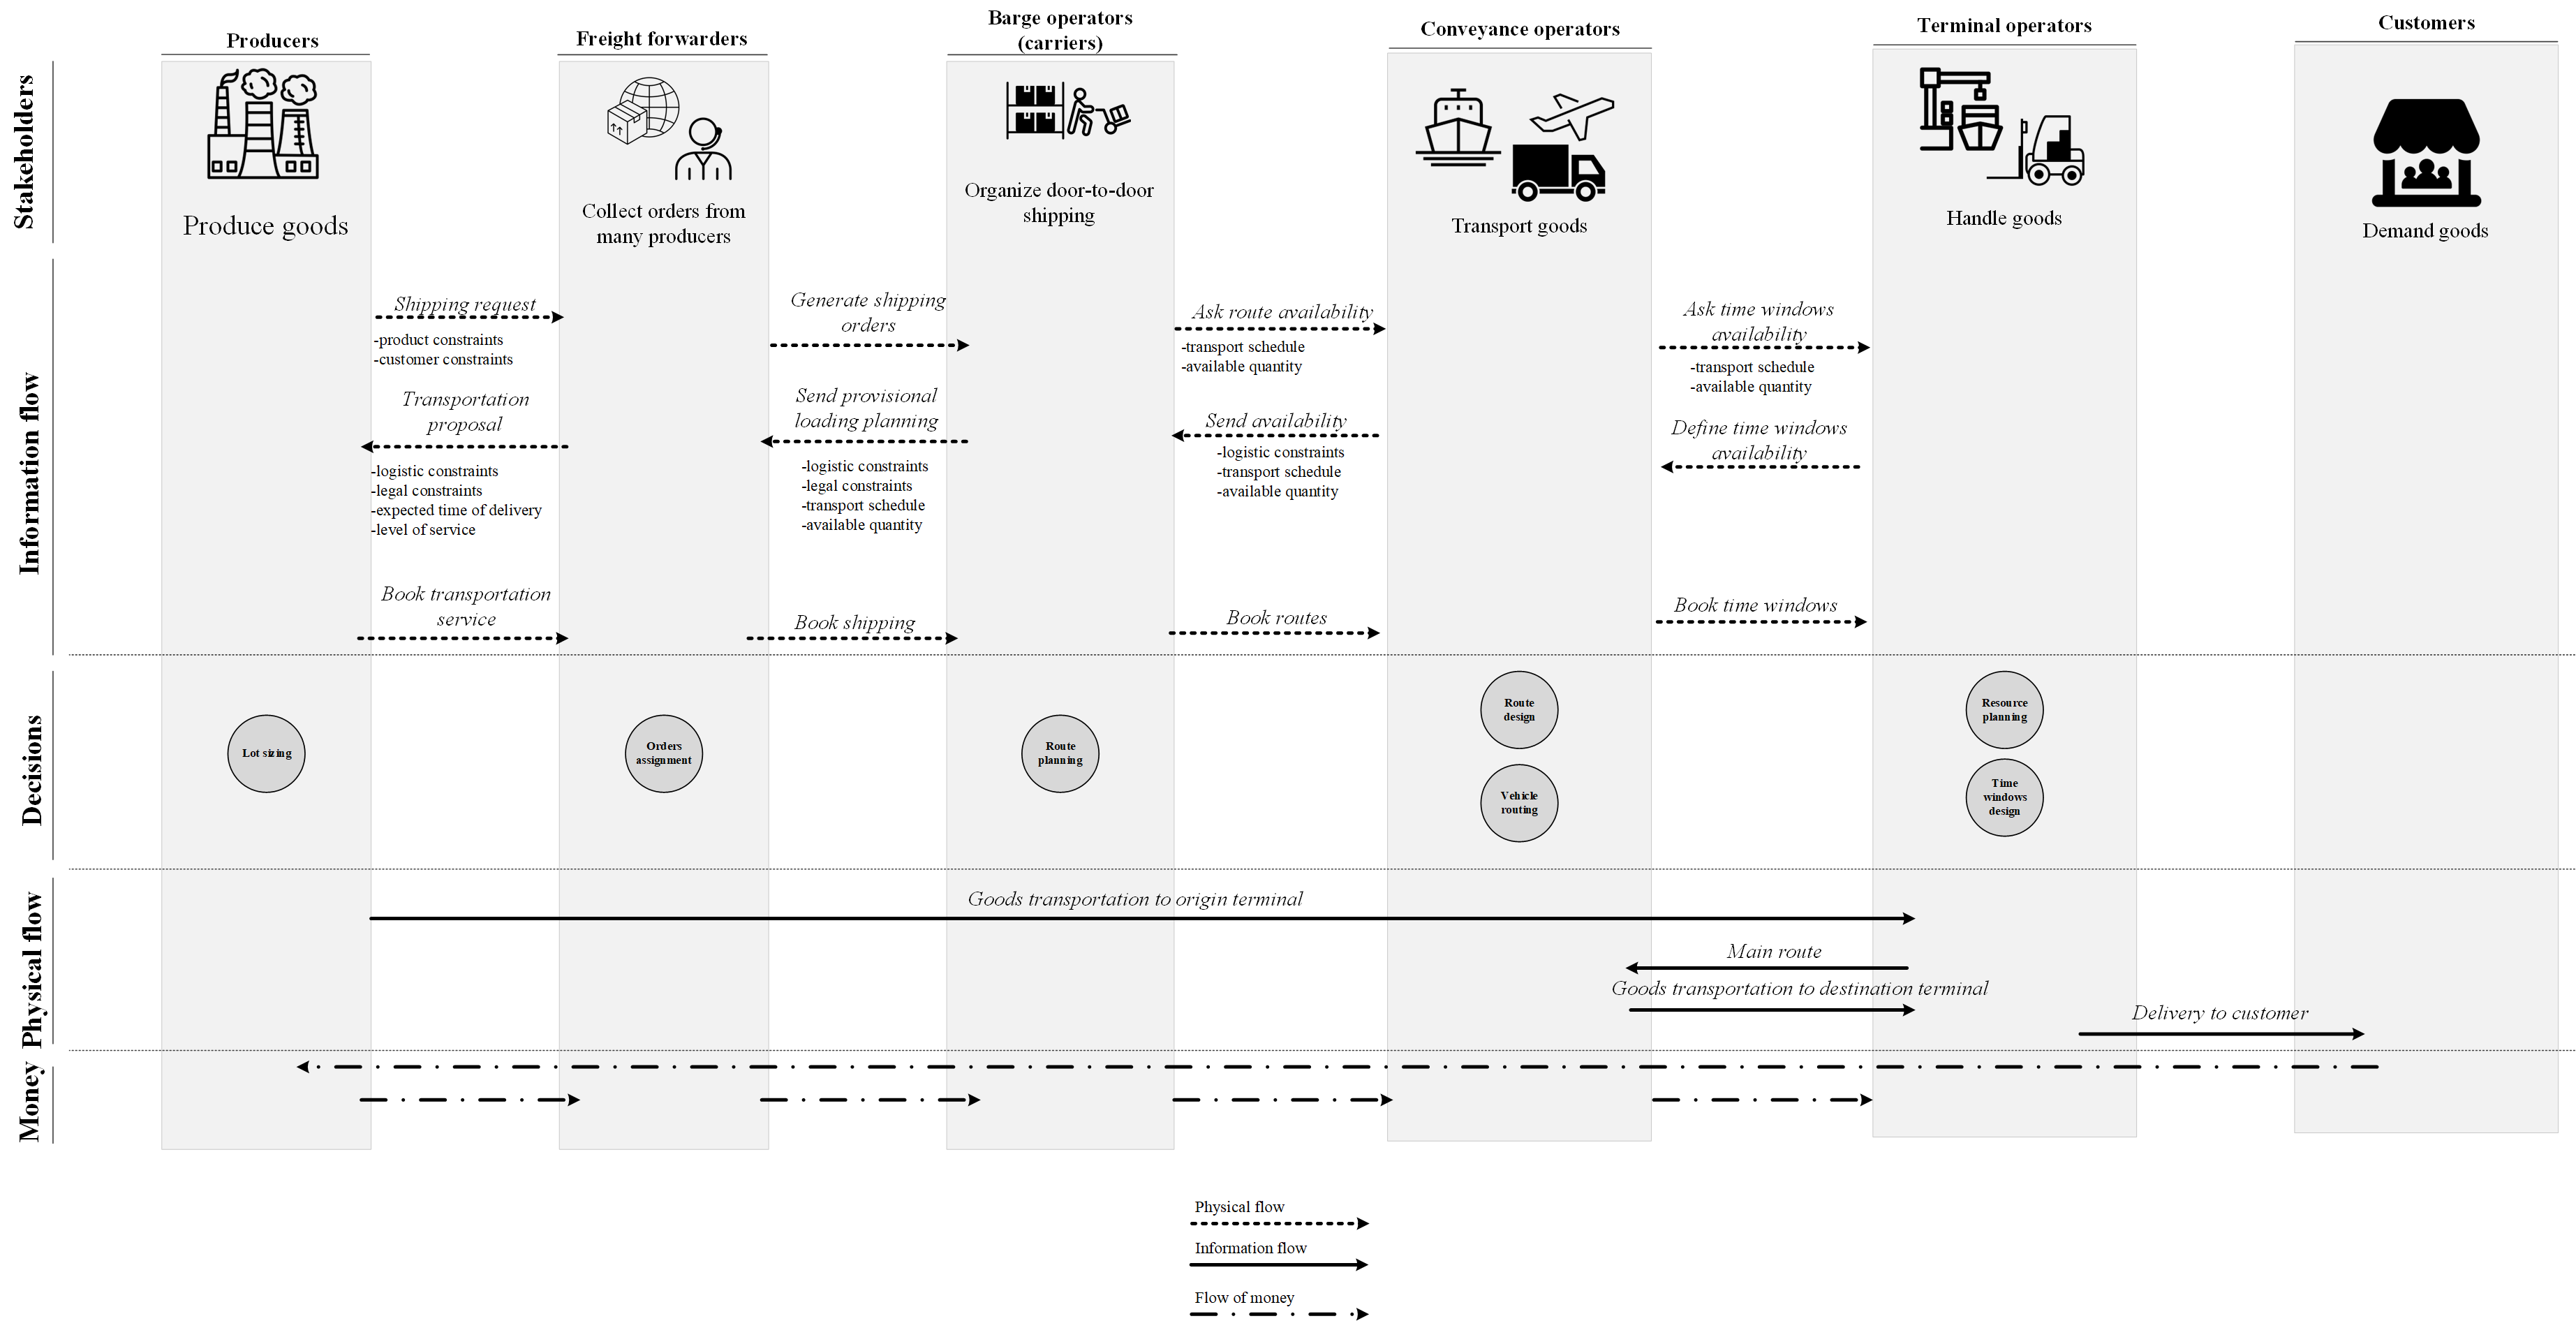
\includegraphics[width=1.7\textwidth]{SectionDistribution/control_figures/fig_actors.png}
\captionsetup{type=figure}
\caption{Stakeholders, logistic flows and related decisions.}
\label{fig_actors}
\end{figure}
\end{landscape}

As Figure \ref{fig_actors} shows, coordination among different actors is a crucial issue to control the operations of a distribution network. The figure remarks the constraints imposed by each actor to the following one depicting the complexity of the system. In practice, a supply chain network is such constrained that can be thought as a system in unstable equilibrium where each actor found its equilibrium within the constraints imposed by the other. Unless a big player has the authority to change these constraints, it is difficult to improve the performance of the supply chain, and it is even challenging to collect the data to control it. During the last few years, the platform economy opened for new opportunities also in this field.\par

\subsection{Logistics platforms} \label{secLogPlatform}
The advent of new technologies as the internet of things, artificial intelligence and fast internet connections paved the way for the so-called “platform revolution”, i.e. the establishment of new business models based on the idea of a platform connecting stakeholders ~\cite{Nambisan2019}. Often, the economic edge of a platform is based on the concept of arbitrage, since platforms can link stakeholders in different ways compared to the established companies in the market ~\cite{Dana2003,Kenney2016}. Platforms started by connecting the end-user to the supplier of a service. It is the case of platforms offering booking services for hotels, taxi or flight that started by offering a link between the supplier and the end-user and consequently started developing complex algorithms based on the collected data to improve their services and their edges ~\cite{Benjaafar2019, Guda2019}. The value of a platform on the market depends on the amount of data it can collect ~\cite{Guda2019}. Recently, platforms started to operate in the business-to-business (B2B) market, too ~\cite{Huang2013}.  In the B2B market, platforms connect companies using different data protocols and complex system by using interfaces and data exchange protocols ~\cite{Yu2007}. \par

The market of logistics has seen a prolific increase in the development and use of logistic platforms during the last decade. A logistic platform is an IT infrastructure to store data and support storage, handling and transport operations across multiple stakeholders.\par

Literature classifies logistic platforms into four classes depending on the functionality they offer ~\cite{Xiu2010}:

\begin{enumerate}
    \item Electronic Data Processing (EDP) platforms; they track the logistic processes storing data into relational databases.
    \item Enterprise Resource Planning (ERP); they integrate all the activities of a stakeholder providing insights and algorithms to improve its performance.
    \item Enterprise Application Integration (EAI); they integrate the activities of a subset of stakeholders enhancing collaborative planning.
    \item Smart Contracts (SC); they fully integrate the tracking of goods processed by the stakeholders of a supply chain providing full visibility on the data and allowing for automatic execution of contracts (e.g., replenishment orders).

\end{enumerate}

Figure \ref{fig_platforms} presents an overview of these functionalities together with the topology and the degree of collaboration offered by each platform.

% INSERT fig_platforms
\begin{landscape}
\thispagestyle{empty}
\begin{figure}[hbt!]
\centering
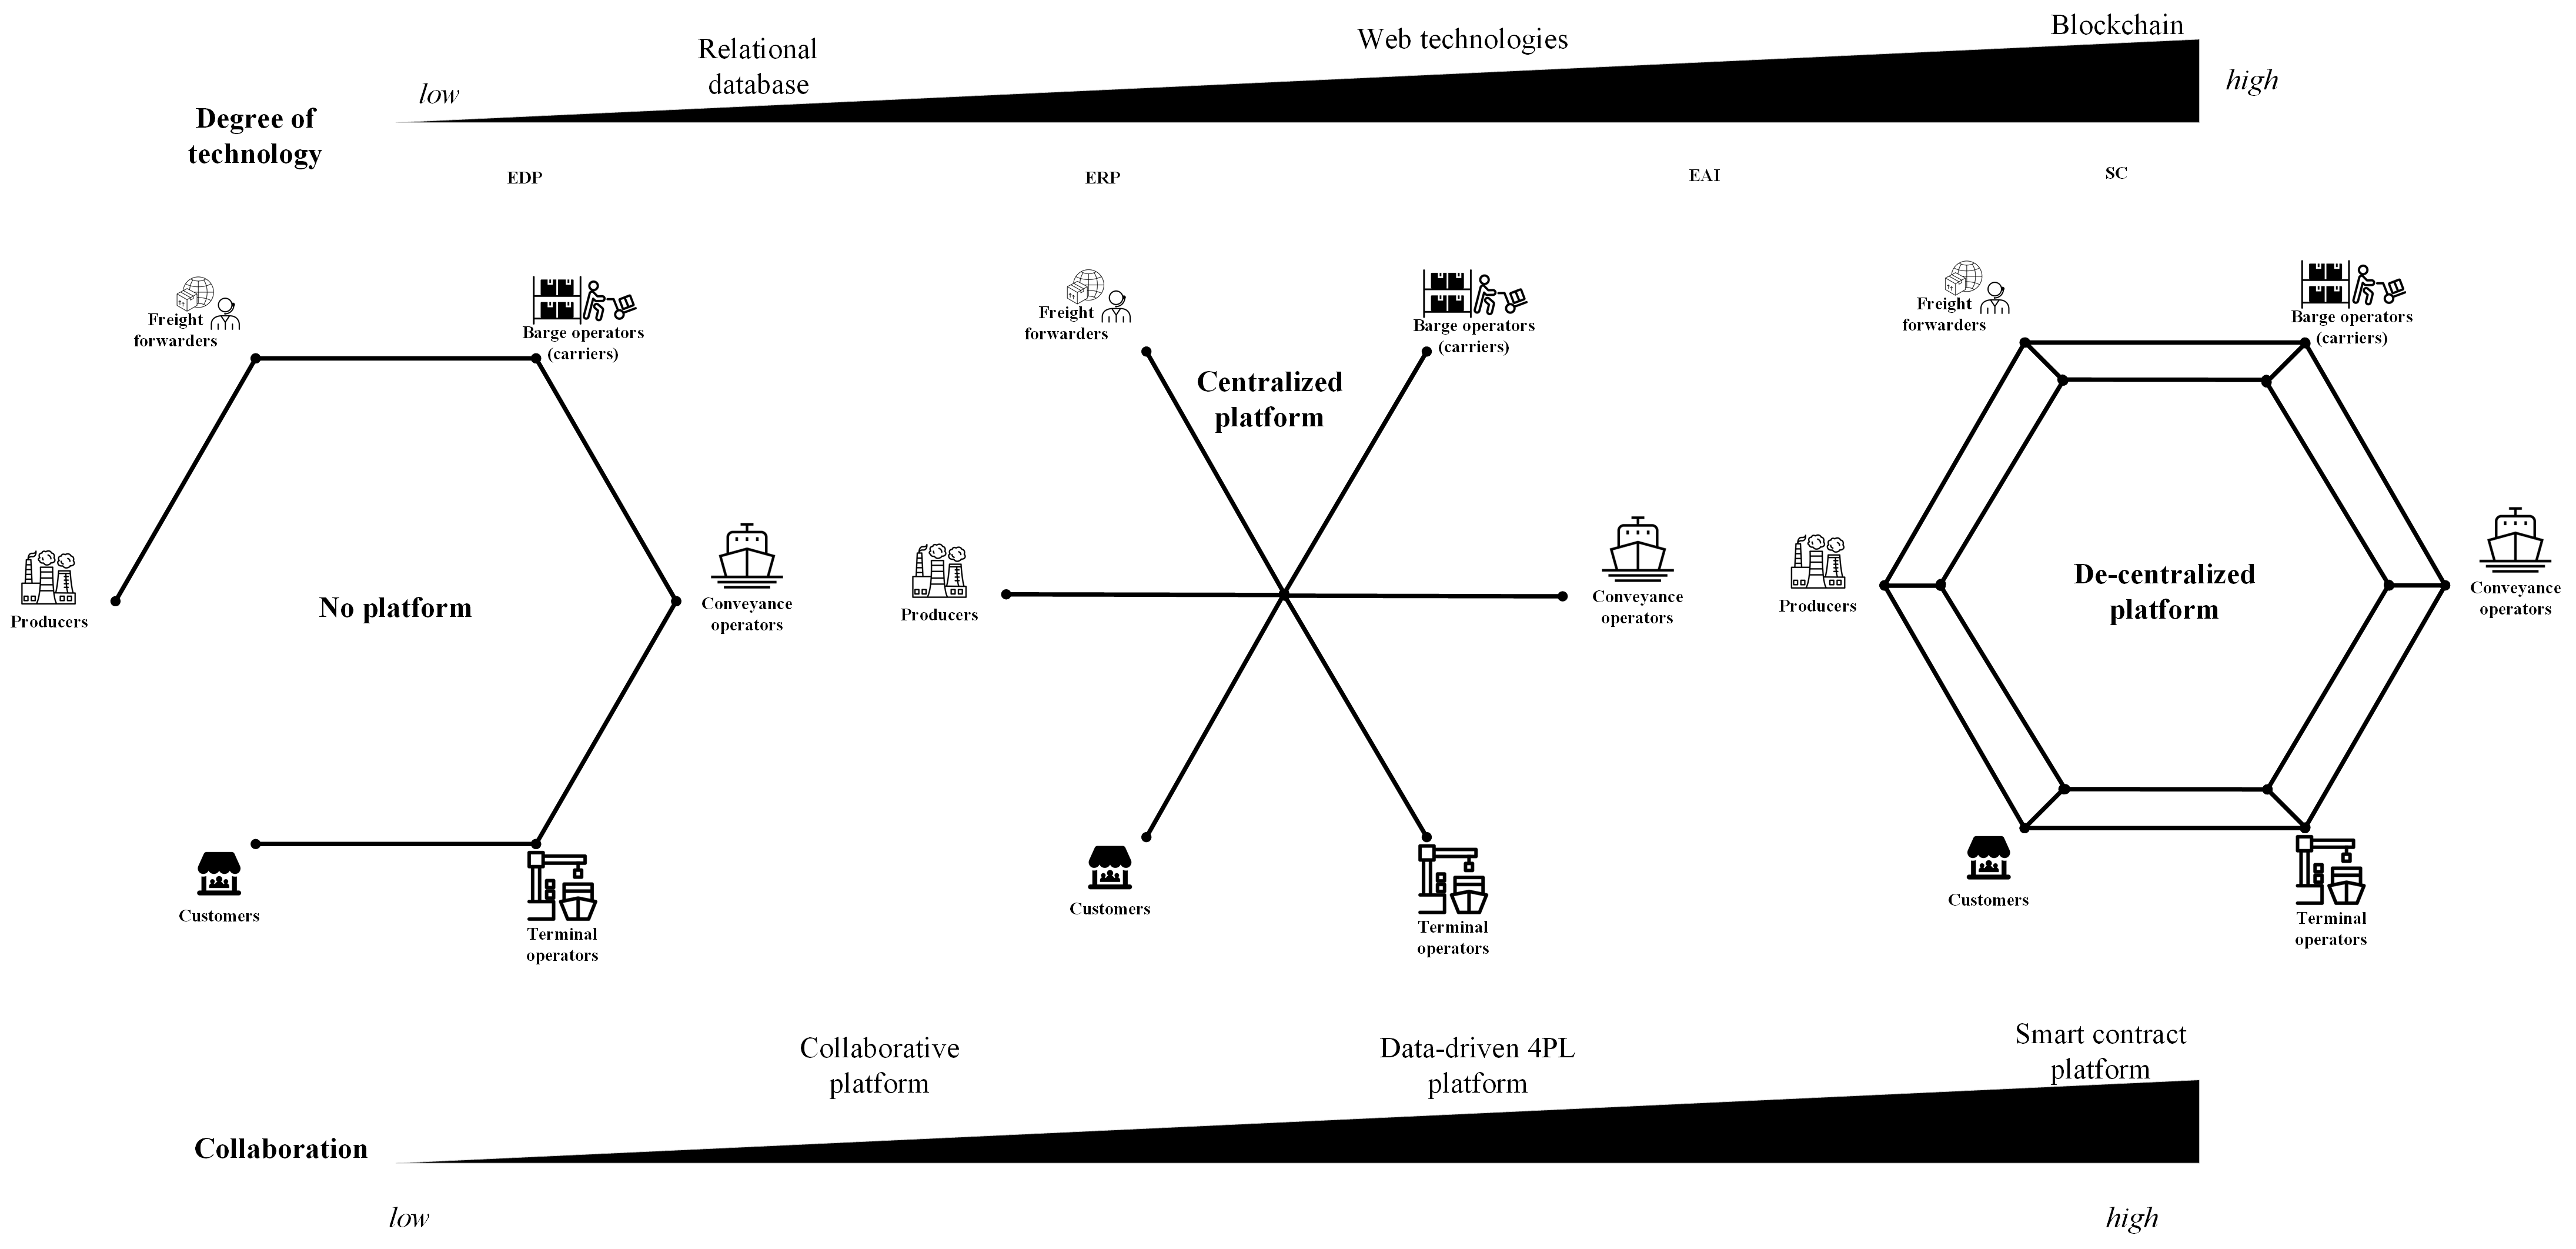
\includegraphics[width=1.6\textwidth]{SectionDistribution/control_figures/fig_platforms.png}
\captionsetup{type=figure}
\caption{An overwiev of logistic platforms.}
\label{fig_platforms}
\end{figure}
\end{landscape}

The topology of logistic platforms changes from a no-platform topology, where data is manually exchanged by the use of telephone, emails and fax \cite{Choy2006, Liu2008}, to centralised platforms where a central entity guarantees the validity of data and transactions between stakeholders. The evolution of this topology is the de-centralised platform where no entity has full control on the platform, but it is distributed among all the stakeholders.\par

De-centralised platforms allow full collaborations between stakeholders using smart contract: each of them has full visibility on the data exchanged by the others, and this provides the highest amount of information for decision making.\par

When stakeholders are not willing to completely share data among them, centralised platforms using incomplete information result adequate. It is the case of collaborative platforms where a low number of stakeholders (typically two) decide to exchange some data to improve their performance. The data-driven 4PL platform is a more complex solution that collects data from many stakeholders providing them with functionalities and services based on big data (impossible to deliver basing only on the data of a few of them). These platforms maintain confidentiality on the data since they are not shared with the other users of the platform.\par

The interest of the scholars on the design and development of logistic platforms increased exponentially during the last decades (see Figure \ref{fig_literatureTrend}.


% INSERT fig_literatureTrend
\begin{figure}[hbt!]
\centering
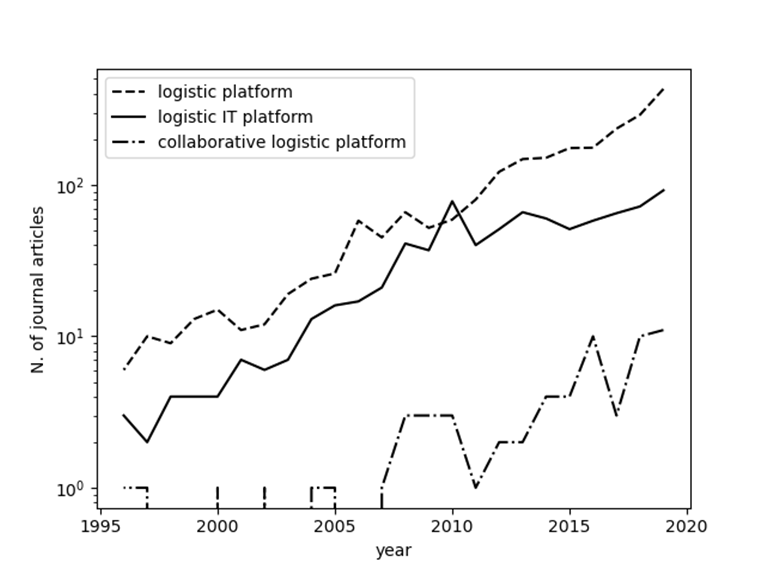
\includegraphics[width=0.9\textwidth]{SectionDistribution/control_figures/fig_literatureTrend.png}
\captionsetup{type=figure}
\caption{Number of journal articles in logarithmic scale obtained using “logistic platform”, “logistic IT platform”, and “collaborative logistic platform” as research queries on Scopus.}
\label{fig_literatureTrend}
\end{figure}

The role of a logistics platform stands in its ability to collect and merge data from different actors and use them to functionalities to them as:

\begin{itemize}
    \item New pricing models \cite{Figliozzi2005, Lindsey2014,Tibben-Lembke2006};
    \item Synchromodality \cite{Giusti2019};
    \item Process integration \cite{Mason2006};
    \item Estimated time of arrival forecast \cite{Pani2014};
    \item Collaborative forecasting and replenishment \cite{Feng2017};
    \item Possibility of last-minute planning \cite{Mulder2019};
    \item Real-time booking (arbitrage) by prediction of the available capacity (this paper);
    \item Digitisation of the processes;
    \item More visibility on the market.

\end{itemize}

All these methods are data-driven and rely on an incomplete but broad data structure. All the data-driven methods presented in the following paragraphs are intended for a logistic platform using a non-relational structure to merge data from different actors of the supply chain.

\subsection{The day-by-day of a distribution network}
Before diving into the math of problems and methods, it is important to understand the operations of a distribution network. For this reason, we introduce some additional details keeping, for example, a port supply chain, one of the most complex types of supply chains. This choice is due to the fact that a port connects thousands of destinations globally distributed using any type of equipment and vehicle to transport any type of good. \par

A port receives physical flows of many types. It always has road and rail connection, at least. Commonly, a port collects goods from inland waterways, and it may be close to an airport collecting air flows. Terminals $j$ process all these flows using storage areas and handling units. Usually, inland terminals pre-process many flows from road and air by consolidating them on barges. Barges, then, reach the deepsea terminal where cargo vessels are loaded and unloaded. Cargo vessels operate:

\begin{itemize}
    \item liner shipping, when routes are predetermined, and the schedule is fixed;
    \item tramp shipping, when shipping is operated on-demand (similarly to charter flights).

\end{itemize}

The complex information flows for booking and tracking is managed by freight forwarders, shipping company and shipbrokers. Figure \ref{fig_portFlows} illustrates the logistic and the information flow of a port supply chain.

% INSERT fig_portFlows


\begin{figure}[hbt!]
\centering
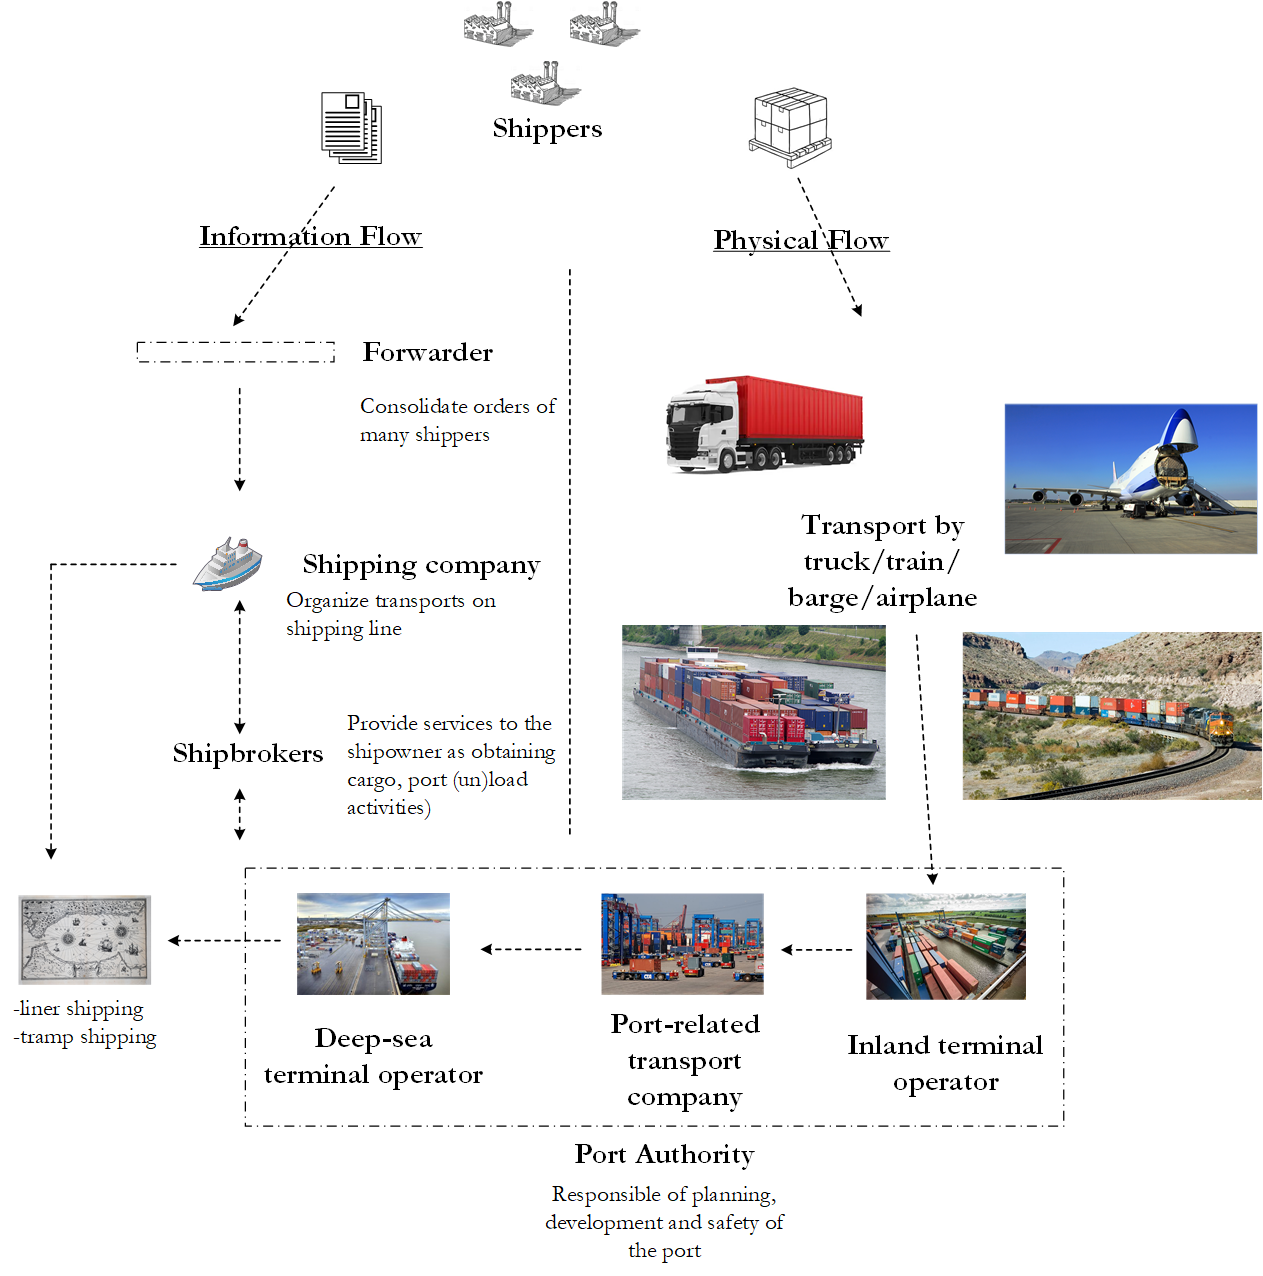
\includegraphics[width=1.0\textwidth]{SectionDistribution/control_figures/fig_portFlows.png}
\captionsetup{type=figure}
\caption{Physical and information flow of a port supply chain.}
\label{fig_portFlows}
\end{figure}

Different types of cargo vessels exist, depending on the type of handling unit they transport. Bulk cargo transport dry or liquid materials as coal, grain or crude oil. Breakbulk cargos are used for steel, wood or other voluminous goods that cannot fit a container. Container cargo vessels load TEU and FEU containers as transport units. Roll-on/off cargo vessels transport vehicles (car and trucks) that drive to enter or exit the vessel. Finally, project cargos are organised for oversize loads. Figure \ref{fig_cargoProducts} illustrates images of the vessels used with different types of products.

%insert figure fig_cargoProducts
\begin{figure}[hbt!]
\centering
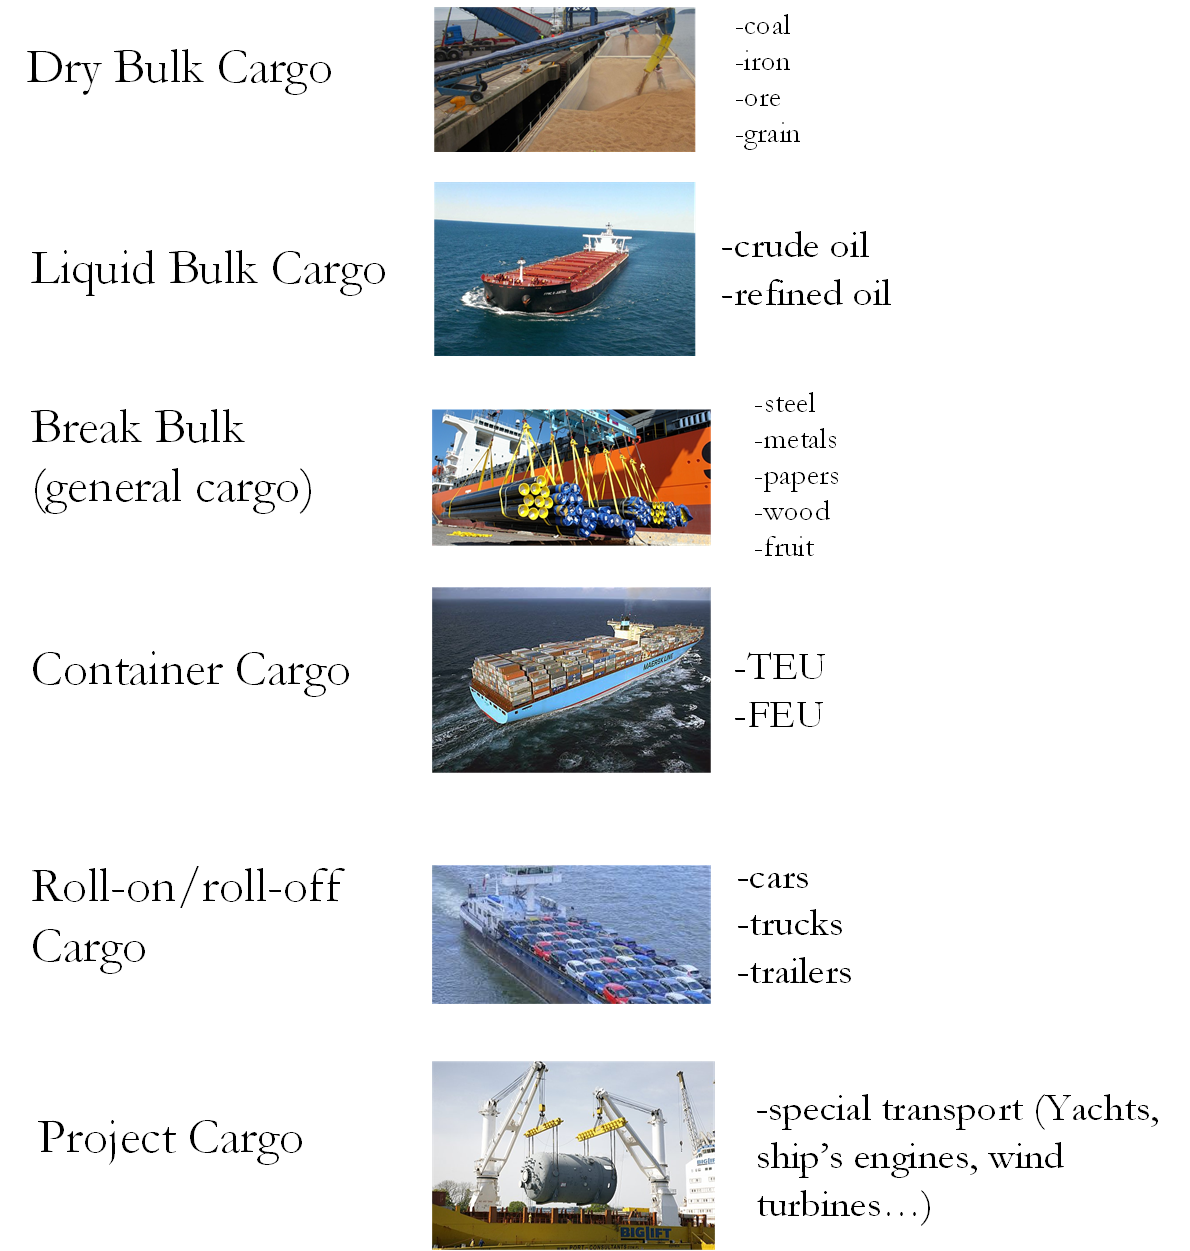
\includegraphics[width=1.0\textwidth]{SectionDistribution/control_figures/fig_cargoProducts.png}
\captionsetup{type=figure}
\caption{Different types of cargo vessels.}
\label{fig_cargoProducts}
\end{figure}

Loading and unloading different types of cargo vessels need a different type of equipment. For this reason, port terminals are specialised on specific types of cargo vessels and specific type of products. Figure \ref{fig_terminalInfrastructure} illustrates the typical equipment of a terminal working with container cargo vessels.

%insert figure fig_terminalInfrastructure
\begin{figure}[hbt!]
\centering
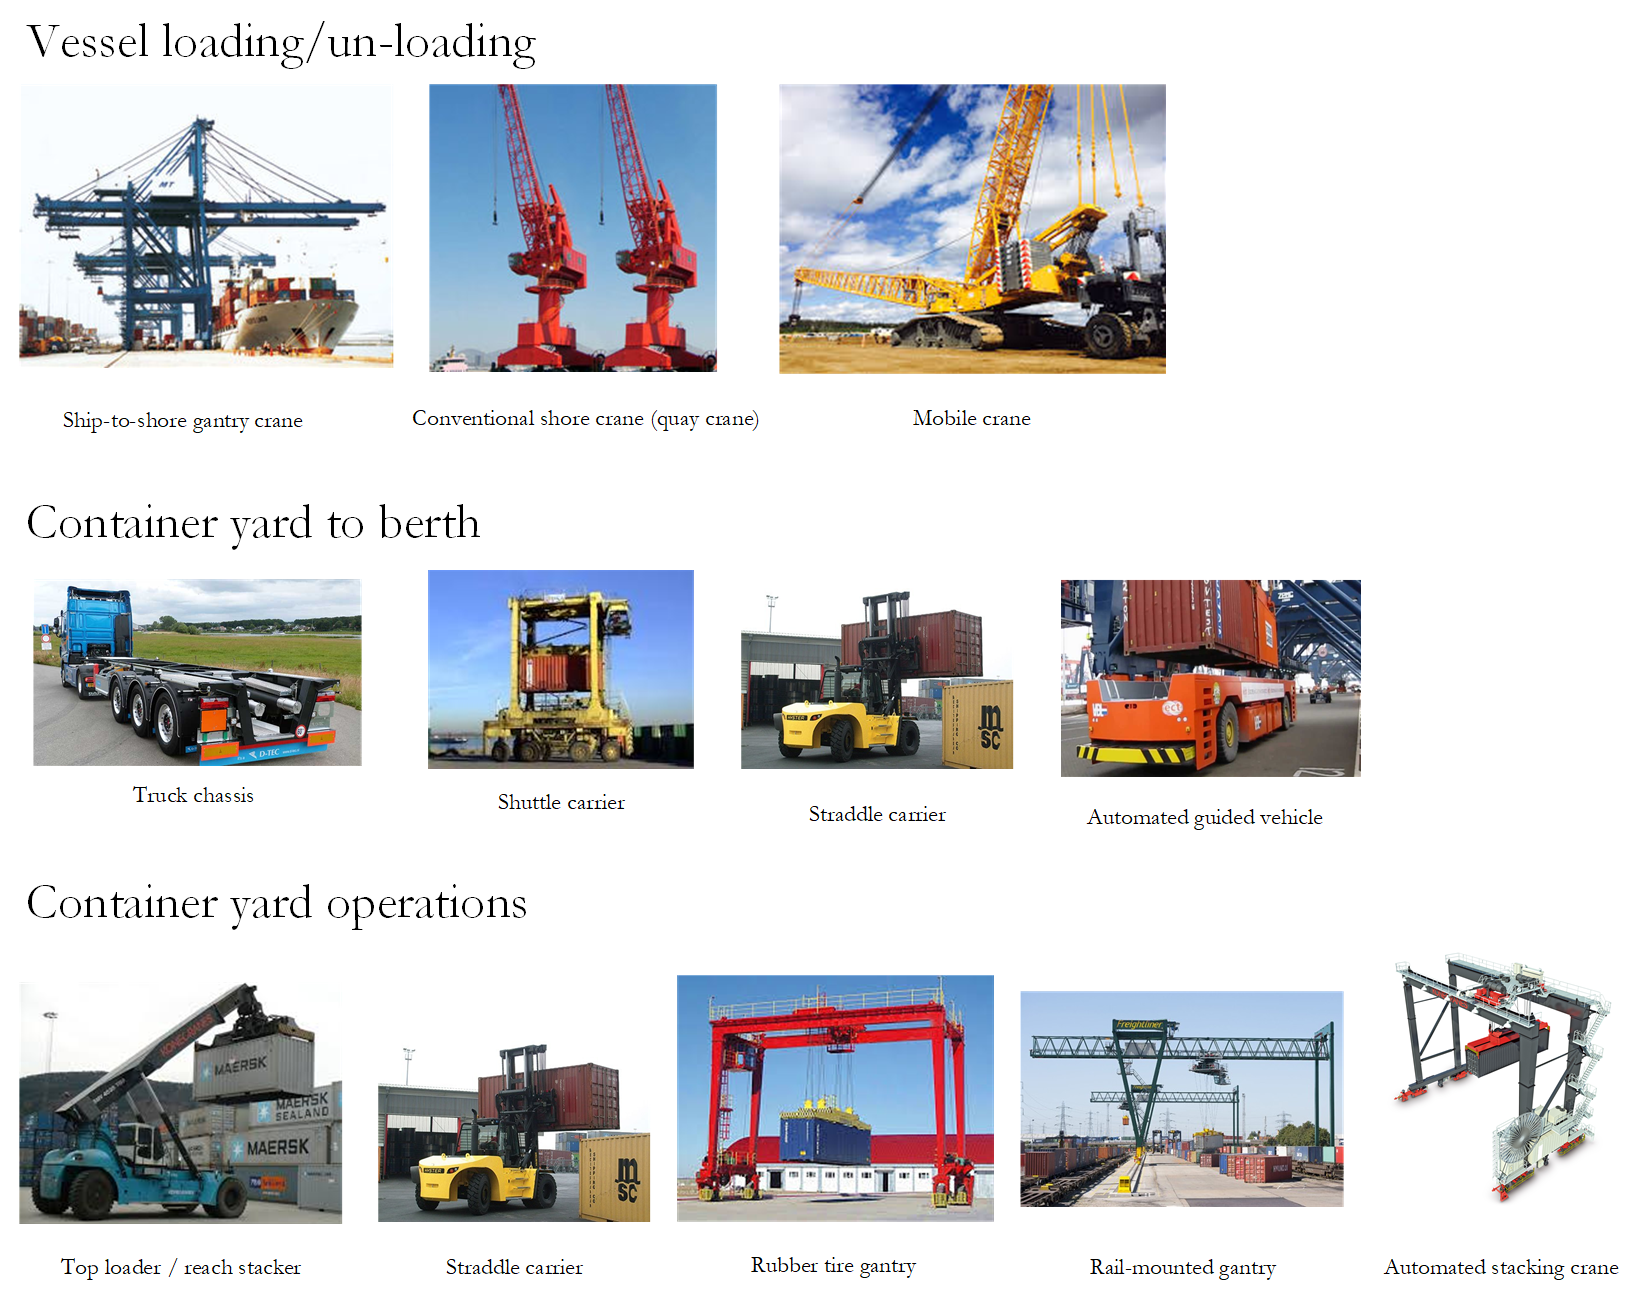
\includegraphics[width=1.0\textwidth]{SectionDistribution/control_figures/fig_terminalInfrastructure.png}
\captionsetup{type=figure}
\caption{Examples of the equipment and physical assets of a port terminal.}
\label{fig_terminalInfrastructure}
\end{figure}

Other supply chain nodes as airport and multimodal hubs are organised similarly. Generally, a logistic hub consists of multiple terminals (generally belonging to different companies) specialised in handling a specific type of product. Terminal companies own the equipment to load and unload cargos and connect a multitude of actors by using freight forwarders and brokers to manage the flow of money and information.

\section{Performance assessment (P8)}

This paragraph introduces models to assess the performance of a supply chain network from a model- and data-driven perspectives.

\subsection{Model-driven methods (D4)}
When the number of actors and flows is high and complex, qualitative business process mapping is always a good starting point to understand what is going on. A common technique is the Business Process Model and Notation (BPMN) (see section \ref{secBPMN}). It remarks the responsibility of each actor and their tasks (e.g. send an order, send confirmation, load container) remarking the activities triggered by each task. Applying the BPMN notation in a distribution network:

\begin{itemize}
    \item activities are tasks necessary for the storage, handling or transportation of a handling unit;
    \item events identify when an activity is terminated (e.g. delivery at the point of consumption, loading completed at a terminal);
    \item gateways describe a different variant of the process (e.g. store in cross-dock or storage area of the terminal depending on the delivery due date).
    \item pools identify the actor of the supply chain in charge of an activity.

\end{itemize}

BPMN defines a qualitative map of the production processes useful for manager and practitioners to identify the way their processes are realised. More difficult is the assessment of these processes from a quantitative point of view. For this reason, a dashboard of KPIs is introduced, coherently with the ontology of \ref{secOntologyDistribution}. The KPIs used in these chapters refers to the problems defined in section \ref{secDecisionPatterns}. KPIs are organised according to four classes ~\cite{Tufano2018}:

\begin{enumerate}
    \item Logistic KPIs, evaluate the logistic impact of a certain solution. They use metrics like time, distance and the performance parameters introduced in section \ref{secOntologyDistribution}.
	\item Cost KPIs, evaluate the economic sustainability of a given solution. They are expressed in \euro{} or other currency.
	\item Energy KPIs, evaluate the energy needed to feed a given solution. They use metrics as kW and kWh.
	\item Environmental KPIs, evaluate the environmental impact of a given solution. They are expressing the equivalent $CO_2$ produced per year.

\end{enumerate}
Table \ref{tab_KPIs} identifies which KPI is relevant to each problem. In general, each problem can be assessed from multiple perspectives.

%insert figure tab_KPIs
\begin{figure}[hbt!]
\centering
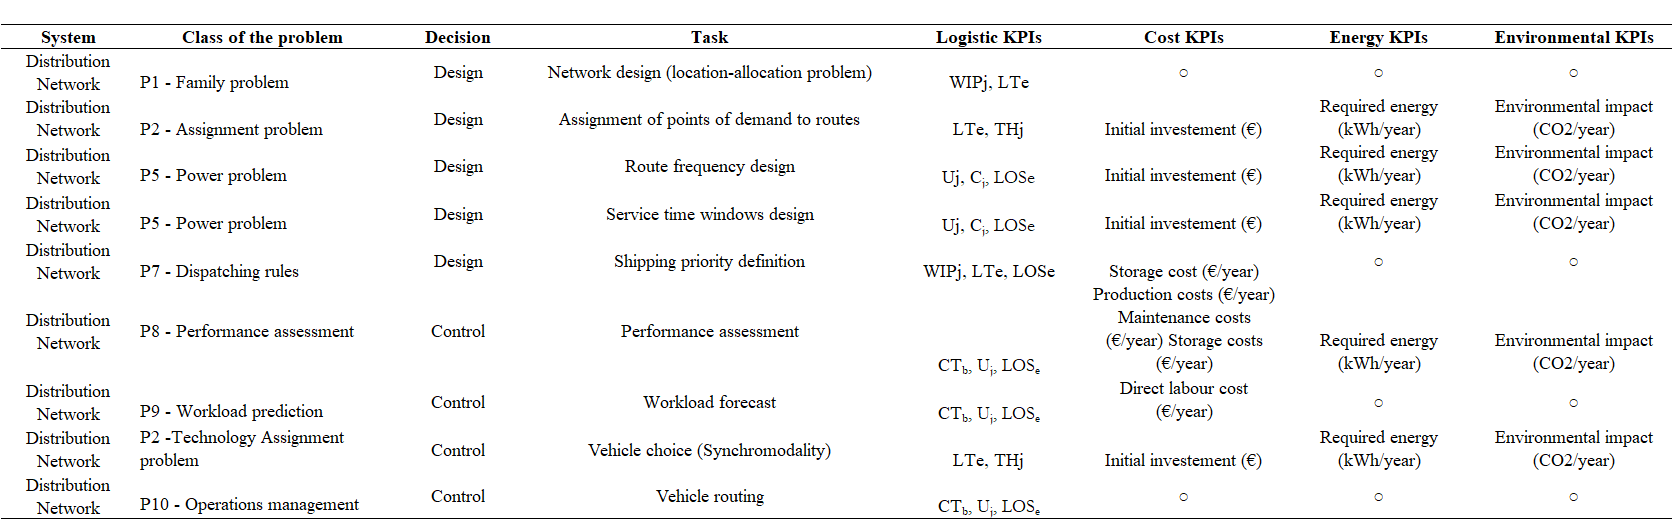
\includegraphics[width=1.0\textwidth]{SectionDistribution/control_figures/tab_KPIs.png}
\captionsetup{type=table}
\caption{KPIs to evaluate the solutions to problems in a distribution network.}
\label{tab_KPIs}
\end{figure}

We show an application of a model-driven method to evaluate the impact of a food supply chain \cite{Baruffaldi2019a, Baruffaldi2019b}. The method relies on the definition of a relational data-structure containing information on:

\begin{itemize}
    \item customer orders, defining the product code and the quantity to transport;
	\item products, including description, volumes, and weights;
	\item transportation units, defining size, capacity concerning the volumes and weights of the products;
	\item vehicles, defining size and capacity concerning the volumes and weights of the transportation units.
	\item impact, defining for each vehicle the cost, and the environmental impact KPIs (e.g. $\frac{CO_2}{ton\times km}$).

\end{itemize}

In practice, the ER structure is organised with a Chinese boxes structure by defining for each vehicle, and for each transportation unit, how many products can be loaded. The model is based on customer orders, and it calculates:

\begin{enumerate}
    \item The number of transportation units necessary to load all the products in the customer orders;
    \item The number of vehicles necessary to transport the transportation units found at 1);
    \item The distance travelled by each vehicle;
    \item The overall cost and impact;
    \item The cost and the impact of each vehicle;
    \item The cost and the impact of each transport unit;
    \item The cost and the impact of each product.

\end{enumerate}

Figure \ref{fig_networkAnalyser} illustrates the entities and the KPIs involved in this model.

%insert figure fig_networkAnalyser
\begin{figure}[hbt!]
\centering
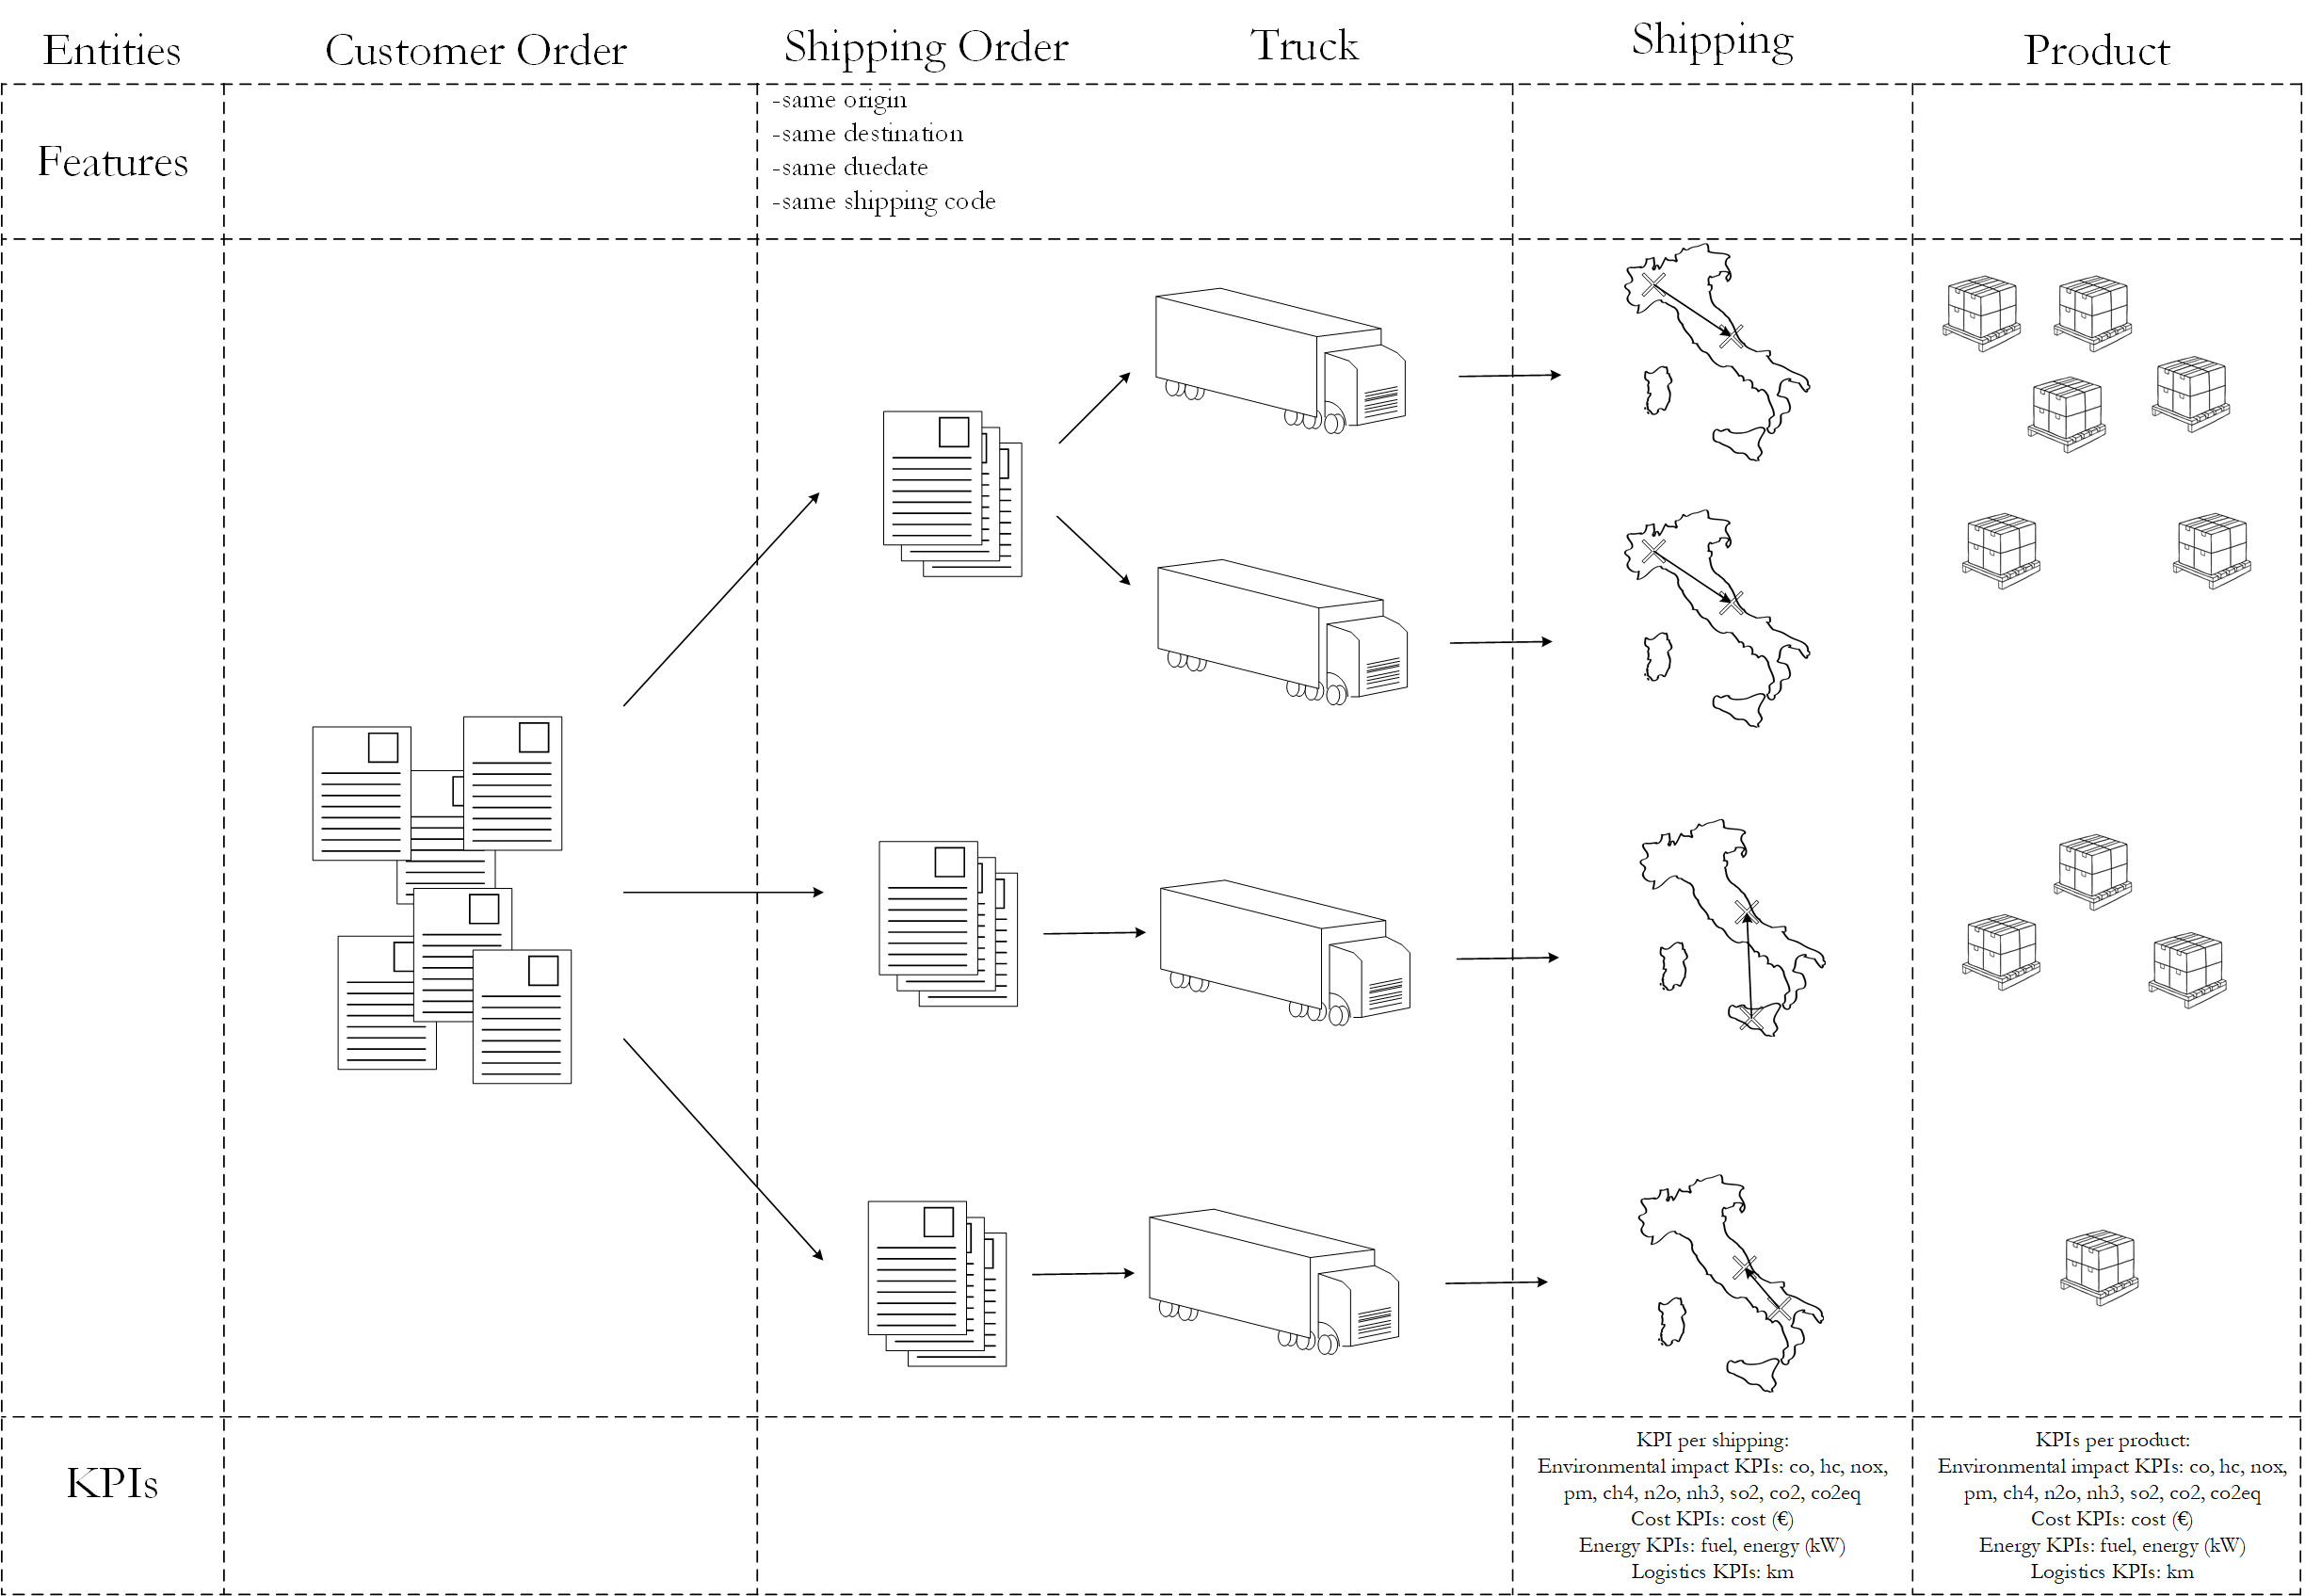
\includegraphics[width=1.0\textwidth]{SectionDistribution/control_figures/fig_networkAnalyser.png}
\captionsetup{type=table}
\caption{Entities and KPIs of the model-driven approach.}
\label{fig_networkAnalyser}
\end{figure}

\subsection{Data-driven methods (D1, D2)}
The aforementioned model-driven approach is punctual and precise. Nevertheless, it relies on a massive amount of static data. All of them are necessary to perform the calculation of the KPIs. In addition, when a parameter is unknown, many hypotheses must be made to run the model, adding bias to the results. To avoid biased results and to expedite the data collection, we introduce a data-driven approach based only on the available data. This method assesses a distribution network from different points of view by considering only the available data, without additional assumptions.There are three macro-areas of analyses:
\begin{enumerate}
    \item the profiling of the actors of the supply chain;
	\item the profiling of the operations of the supply chain;
    \item the profiling of the geographical network of the supply chain.

\end{enumerate}

The presence in the dataset of certain attributes allows the realisation of some analyses. We can think of attributes as keys and analysis as doors; the right keys unlock the right doors. Figure \ref{fig_diagnosisDataDriven} illustrates the links between attributes and analysis (keys and doors), illustrated in details in the following paragraphs.

%insert figure fig_diagnosisDataDriven
\begin{landscape}
\thispagestyle{empty}
\begin{figure}[hbt!]
\centering
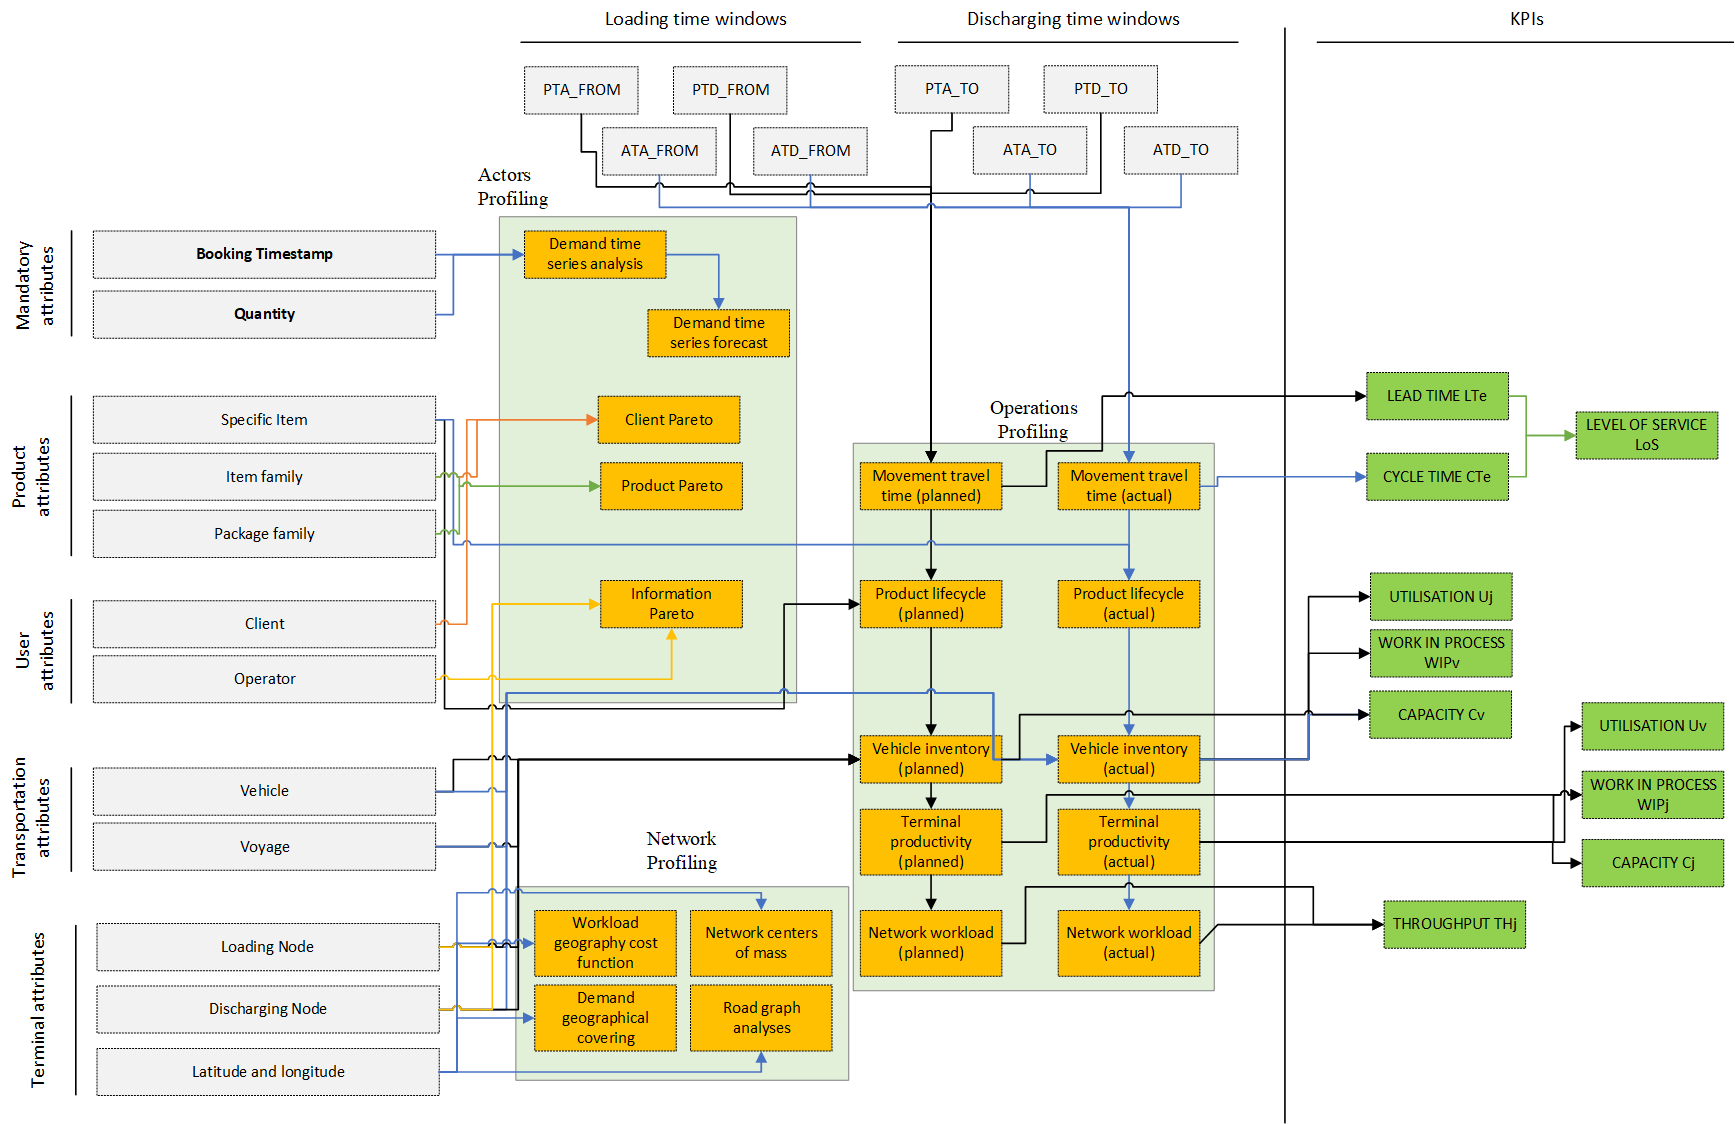
\includegraphics[width=1.5\textwidth]{SectionDistribution/control_figures/fig_diagnosisDataDriven.png}
\captionsetup{type=figure}
\caption{Connections between attributes, analyses and KPIs.}
\label{fig_diagnosisDataDriven}
\end{figure}
\end{landscape}

\subsubsection{Actors Profiling}

\paragraph{Demand time series analysis and forecast}

To support our data-driven approach, we base on the definition of the MVM of the collection movement, defined in \ref{secOntologyDistribution}. The MVM prescribe two mandatory attributes:

\begin{itemize}
    \item a timestamp describing when the movement is created (i.e. when an order arrives from a client);
    \item the quantity involved.

\end{itemize}

By using these two attributes, it is possible to analyse the demand time series and use this information to make forecasts (see section \ref{secDistWorkloadPrediction}). Analysis should be performed on:

\begin{itemize}
    \item the number of lines, i.e. the count of the timestamps;
    \item the quantities, i.e. the sum of the quantity processed at the same timestamps.

\end{itemize}

These two analyses are always relevant since the business of the companies can be line-oriented (e.g. it is the case of third party logistics) or quantity-oriented (e.g. for production industry). Timeseries must always be resampled using an aggregation function. The sampling interval depends on the amount of data collected and on the relevance of the analysis. Frequent sampling intervals are the day, the week or the month. Figure \ref{fig_demandTimeseries} illustrate the daily, weekly and monthly trends of the number of movement with their probability distributions. The bottom of Figure \ref{fig_demandTimeseries} shows the comparison between the lines and quantity trends, and a histogram of the number of movements per day of the week.\footnote{The source code of Figure \ref{fig_demandTimeseries} is available \href{https://github.com/aletuf93/logproj/blob/master/examples/LOG_01\%20Demand\%20assessment.ipynb}{here}.}

%insert figure fig_demandTimeseries
\begin{figure}[hbt!]
\centering
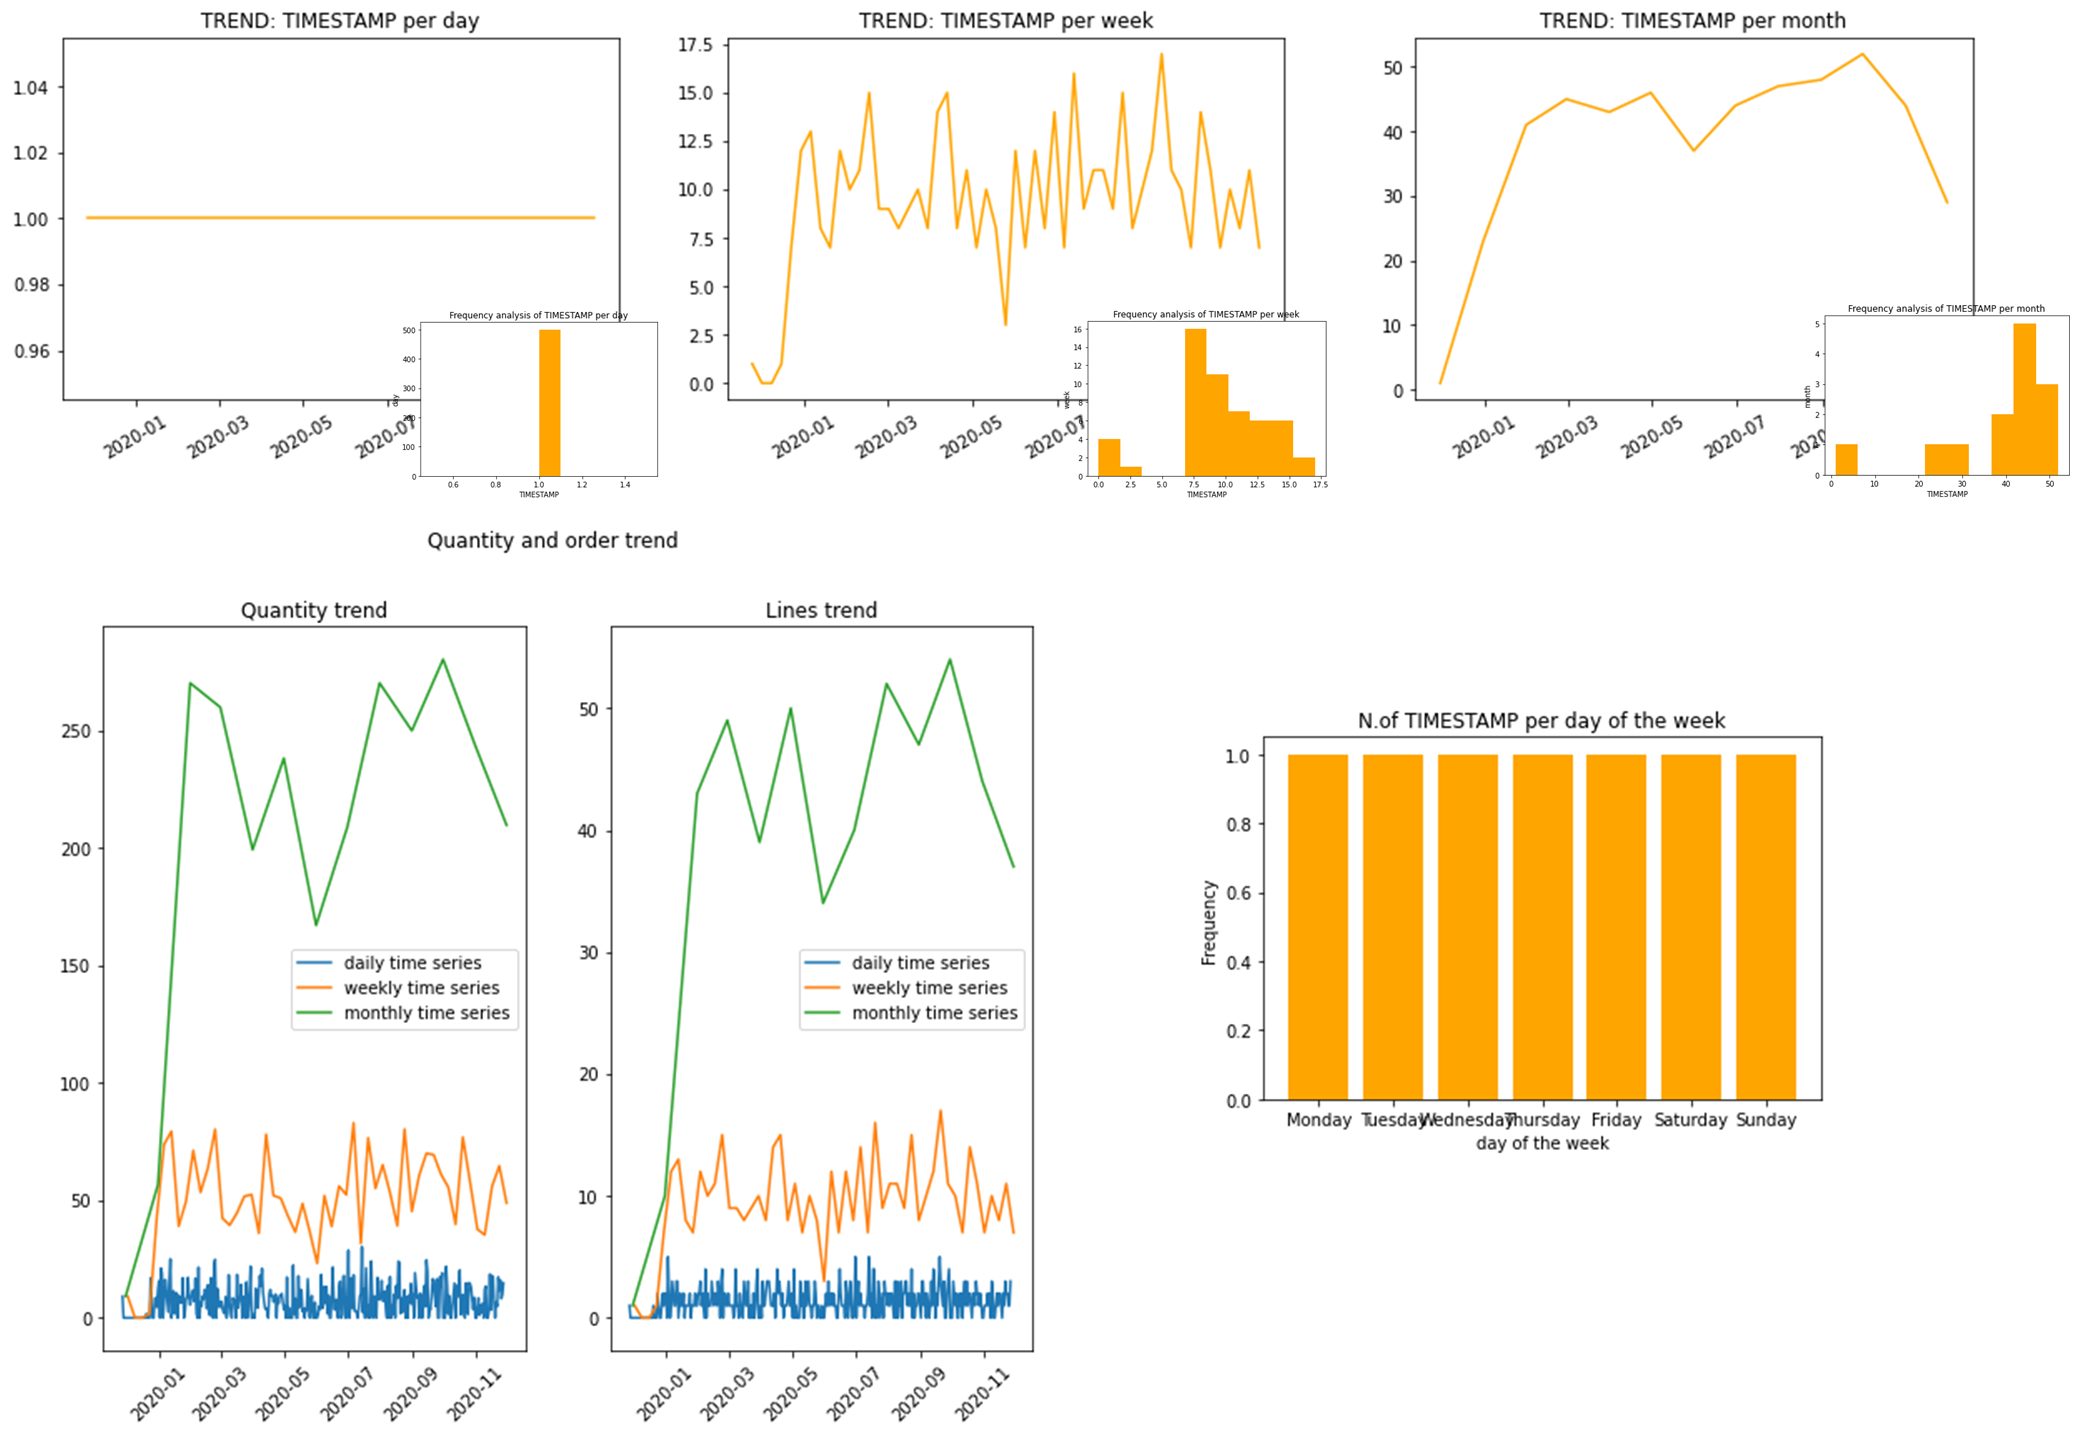
\includegraphics[width=0.9\textwidth]{SectionDistribution/control_figures/fig_demandTimeseries.png}
\captionsetup{type=figure}
\caption{Time series and probability distributions of the movements of a distribution network, using different aggregation levels.}
\label{fig_demandTimeseries}
\end{figure}

These time series can be analysed, and decomposed to uncover trend and seasonality patterns. Figure \ref{fig_demandDecomposition} illustrates the decomposition of the weekly aggregated lines and quantities time series with the Fourier analysis.\footnote{The source code of Figure \ref{fig_demandDecomposition} is available \href{https://github.com/aletuf93/logproj/blob/master/examples/LOG_01\%20Demand\%20assessment.ipynb}{here}.}

%insert figure fig_demandDecomposition
\begin{figure}[hbt!]
\centering
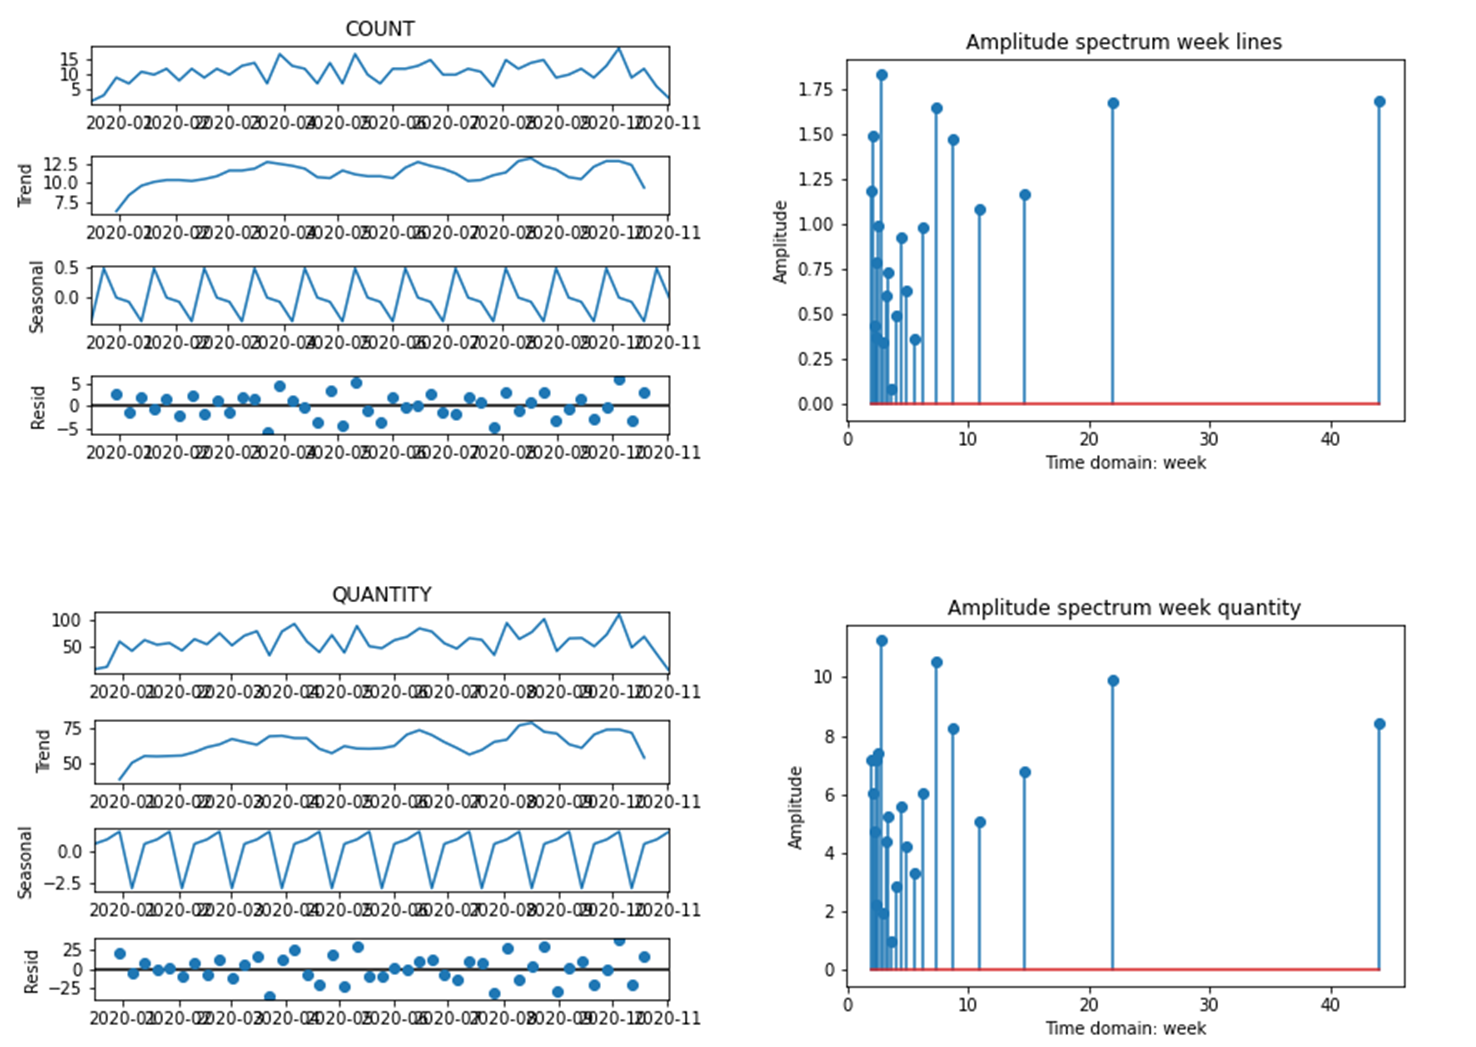
\includegraphics[width=0.9\textwidth]{SectionDistribution/control_figures/fig_demandDecomposition.png}
\captionsetup{type=figure}
\caption{Time series decomposition, and Fourier analysis of the movements.}
\label{fig_demandDecomposition}
\end{figure}

By considering the time series and all the available attributes of the dataset, it is possible to define a correlation matrix to uncover hidden patterns and behaviours of the network (see Figure \ref{fig_demand_correlation}).\footnote{The source code of Figure \ref{fig_demand_correlation} is available \href{https://github.com/aletuf93/logproj/blob/master/examples/LOG_01\%20Demand\%20assessment.ipynb}{here}.}

%insert figure fig_demand_correlation
\begin{figure}[hbt!]
\centering
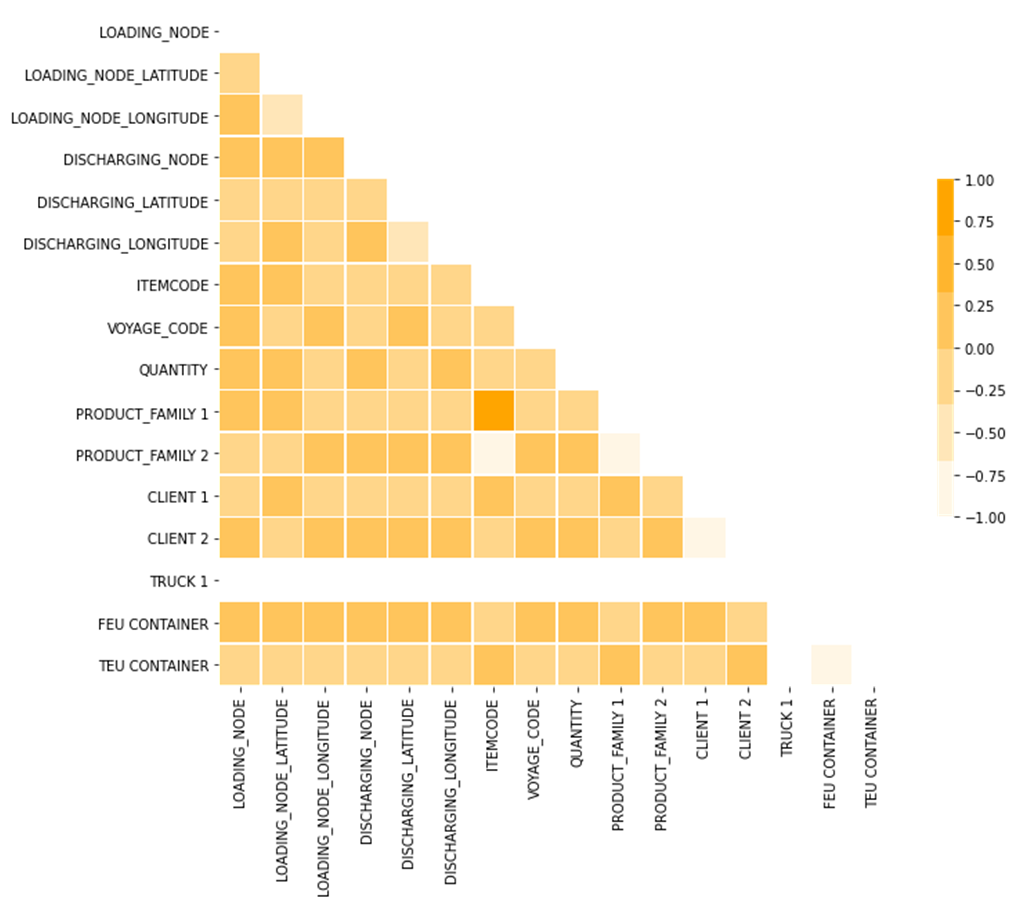
\includegraphics[width=0.9\textwidth]{SectionDistribution/control_figures/fig_demand_correlation.png}
\captionsetup{type=figure}
\caption{Correlation matrix of the movements dataset.}
\label{fig_demand_correlation}
\end{figure}

\clearpage %start a new page
\paragraph{Client Pareto}
Time series analysis focuses on the workload. From another perspective, it is important to identify the source of the workload. Clients define the market demand and, almost always, their relevance follows the Pareto law: 20\% of the customers generate 80\% of the workload. Having information both on the quantities and the clients allows identifying the relative importance of each client. Figure \ref{fig_paretoClient} presents this information using a pie chart and a Pareto curve.\footnote{The source code of Figure \ref{fig_paretoClient} is available \href{https://github.com/aletuf93/logproj/blob/master/examples/DIST_01\%20Supply\%20Chain\%20Assessment.ipynb}{here}.}

%insert figure fig_paretoClient
\begin{figure}[hbt!]
\centering
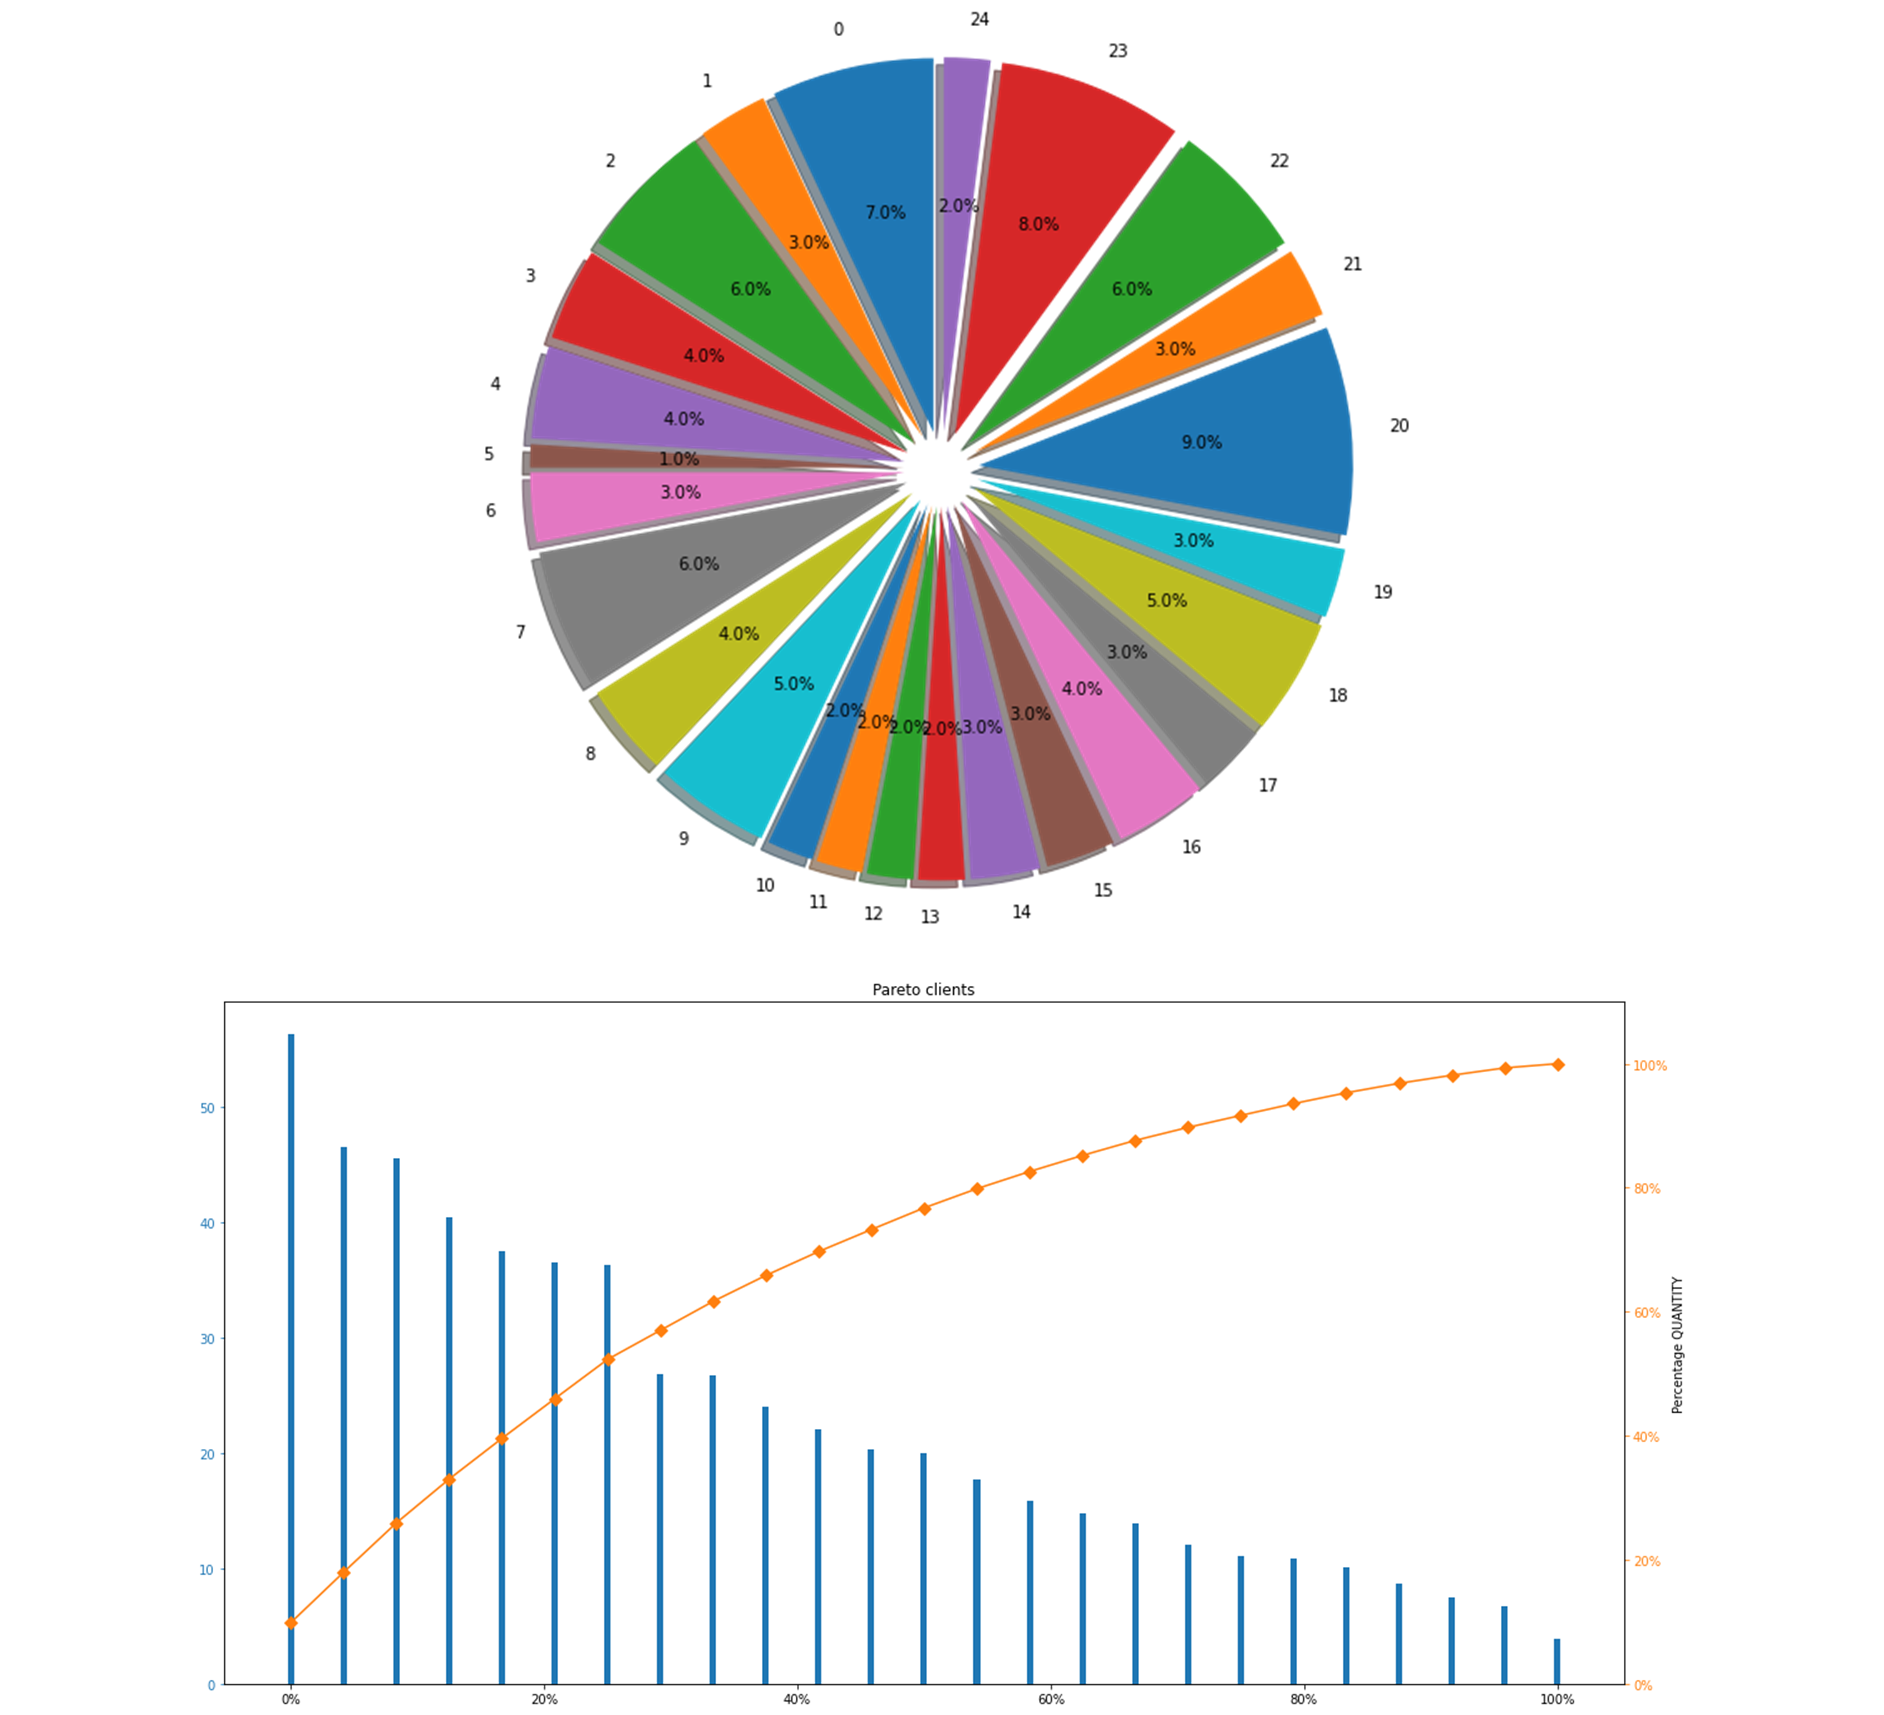
\includegraphics[width=0.9\textwidth]{SectionDistribution/control_figures/fig_paretoClient.png}
\captionsetup{type=figure}
\caption{Pie chart and Pareto curve of a set of clients.}
\label{fig_paretoClient}
\end{figure}

Similar information may be of interest when referred to a single terminal of the distribution network. Figure \ref{fig_violinClient} illustrates the violin chart of the four most congested terminals of a distribution network. The chart identifies the demand (e.g. the quantity or the number of movements) of each client assigned to each terminal. \footnote{The source code of Figure \ref{fig_violinClient} is available \href{https://github.com/aletuf93/logproj/blob/master/examples/DIST_01\%20Supply\%20Chain\%20Assessment.ipynb}{here}.}

%insert figure fig_violinClient
\begin{figure}[hbt!]
\centering
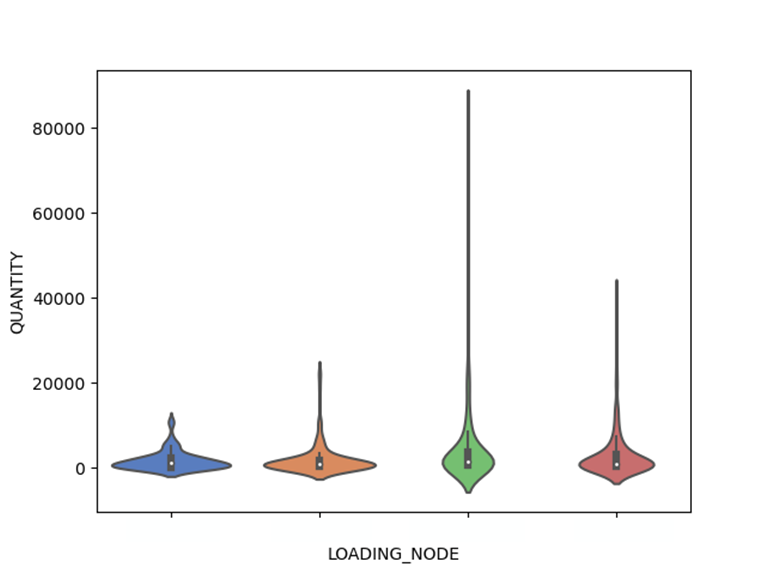
\includegraphics[width=0.9\textwidth]{SectionDistribution/control_figures/fig_violinClient.png}
\captionsetup{type=figure}
\caption{Violin chart with demand for each client for each terminal.}
\label{fig_violinClient}
\end{figure}

\paragraph{Product Pareto}

If clients define the market demand, products define the offer. Again, it is common that 20\% of the products realise 80\% of sales the volumes. The Pareto analysis helps to identify these products. Similar analyses to Figures \ref{fig_paretoClient}, and \ref{fig_violinClient} can be used to map the product mix.

\paragraph{Information Pareto}
Pareto analysis is important to assess the relevance of the information and the statistical coverage of any analysis. Let us define the “operators” as the different users uploading information in the dataset. When working with a supply chain network, it is easy to have many operators since there are tens of actors and multiple data sources. Each actor has a different relevance in terms of:

\begin{enumerate}
    \item The number of records uploaded;
    \item The amount of information generated by the records uploaded.
\end{enumerate}

The last metric is not trivial since it considers the information added by a single operator compared to the information already known in the dataset. This metric is important when data are incomplete. Let assume we want to identify the route travelled by truck transporting a number of HUs. The truck receives order from multiple stakeholders. These stakeholders are operators since they upload data to our dataset.\par 

Assuming a single stakeholder load the 80\% of the truck, the amount of information generated by that single user is much more relevant than the others. The other operators have a low probability of adding information if a single operator generates 80\% of the knowledge. Figure \ref{fig_information} illustrates the behaviour of the information provided by different users of a vehicle. The first three users cover 80\% of all the destinations of the vehicle, providing the principal amount of information on its route. Even without the information provided by the last three users, it is possible to use the data to estimate the route of the vehicle correctly. \footnote{The source code of Figure \ref{fig_information} is available \href{https://github.com/aletuf93/logproj/blob/master/examples/DIST_01\%20Supply\%20Chain\%20Assessment.ipynb}{here}.}

%insert figure fig_information
\begin{figure}[hbt!]
\centering
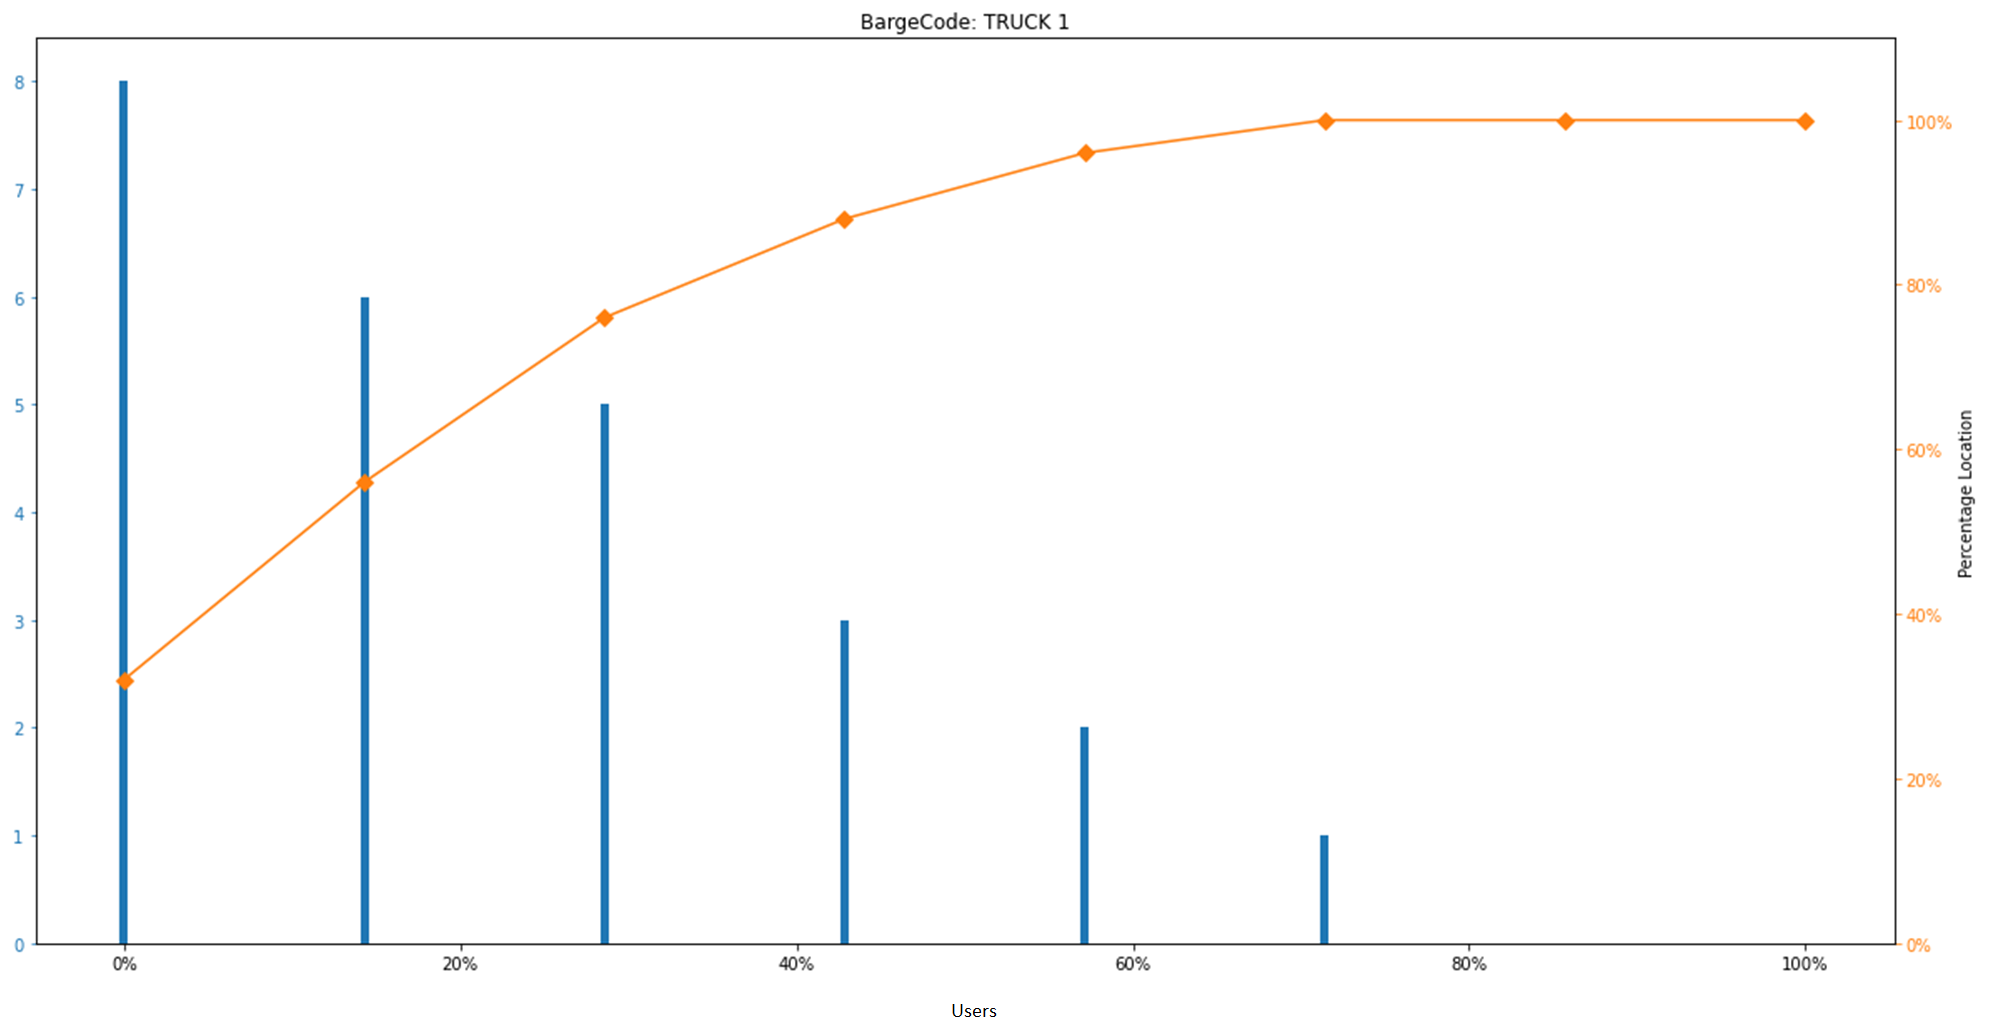
\includegraphics[width=0.9\textwidth]{SectionDistribution/control_figures/fig_information.png}
\captionsetup{type=figure}
\caption{Information Pareto on client and vessel route.}
\label{fig_information}
\end{figure}

\subsubsection{Operations profiling} \label{secDistOperationsProfiling}
\paragraph{Movement Travel Time analysis}
The analysis of the travel time reveals the time each HU $i$ spend on a vehicle. By knowing the loading time window at node $j$, and the discharging time windows at the node $k$, it is possible to calculate the upper bound $TT^{UB}$ and the lower bound $TT^{LB}$ of the travel time as:
\begin{itemize}
    \item $	TT_\pi^{UB}=PTD_{ik}^{TO}-PTA_{ij}^{FROM}$
    \item $	TT_\pi^{LB}=PTA_{ik}^{TO}-PTD_{ij}^{FROM}$
\end{itemize}

By aggregating these analyses, it is possible to identify the lead time $LT_e$ of a route $e$. By knowing the actual time windows, the analysis can be repeated using:  
\begin{itemize}
    \item $TT_\alpha^{UB}=ATD_{ik}^{TO}-ATA_{ij}^{FROM}$
    \item $TT_\alpha^{LB}=ATA_{ik}^{TO}-ATD_{ij}^{FROM}$
\end{itemize}

Figure \ref{fig_travelTime} compares the planned and actual travel time for the HUs handled in a distribution network. \footnote{The source code of Figure \ref{fig_travelTime} is available \href{https://github.com/aletuf93/logproj/blob/master/examples/DIST_01\%20Supply\%20Chain\%20Assessment.ipynb}{here}.}

%insert figure fig_travelTime
\begin{figure}[hbt!]
\centering
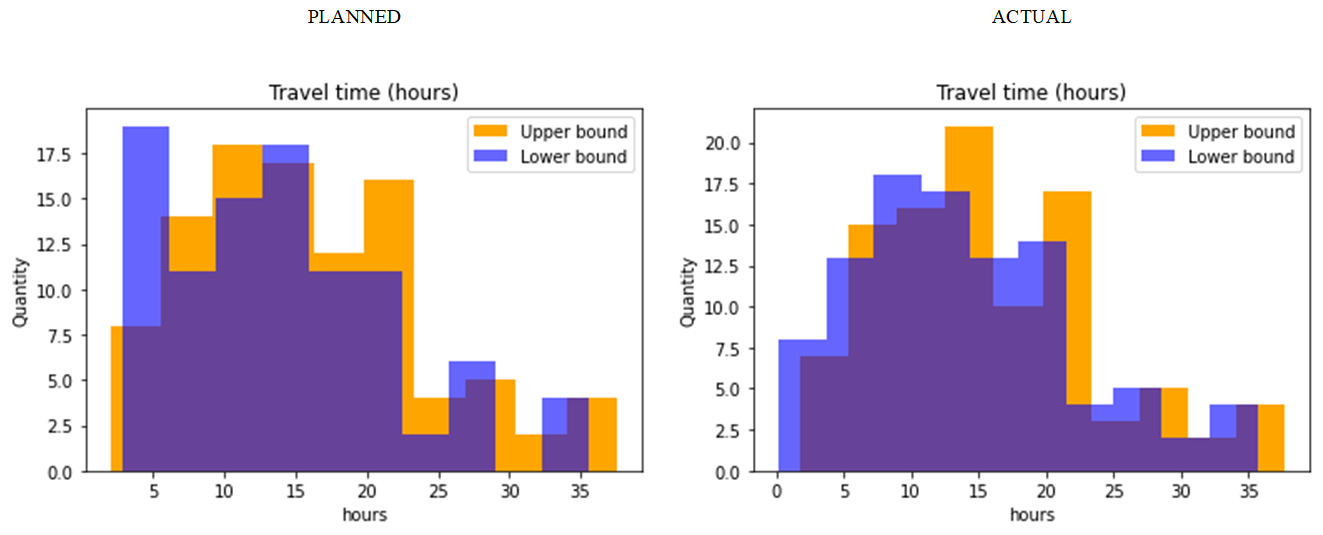
\includegraphics[width=0.9\textwidth]{SectionDistribution/control_figures/fig_travelTime.png}
\captionsetup{type=figure}
\caption{Planned and actual travel time.}
\label{fig_travelTime}
\end{figure}

By aggregating the actual travel times, the cycle time $CT_e$ of a route e is revealed. By considering all the route e of a network $G$, the level of service of the network is calculated as the $Prob{CT_e\le LT_e}$ (see Figure \ref{fig_serviceLevel}).\footnote{The source code of Figure \ref{fig_serviceLevel} is available \href{https://github.com/aletuf93/logproj/blob/master/examples/DIST_01\%20Supply\%20Chain\%20Assessment.ipynb}{here}.}

%insert figure fig_serviceLevel
\begin{figure}[hbt!]
\centering
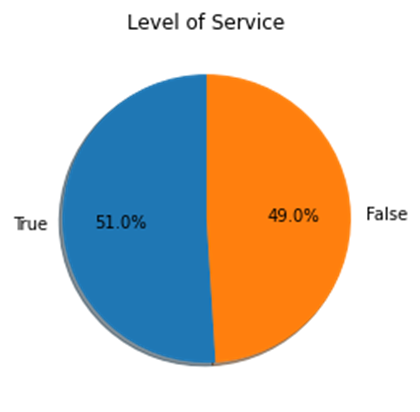
\includegraphics[width=0.4\textwidth]{SectionDistribution/control_figures/fig_serviceLevel.png}
\captionsetup{type=figure}
\caption{Pie chart representing the level of service of the ditribution network.}
\label{fig_serviceLevel}
\end{figure}

\paragraph{Product Lifecycle analysis}
When the dataset contains a different code (specific item) for each different HU transported on the network, it is possible to have full traceability of the network and to reconstruct all the distribution stages. In particular, by knowing the loading and unloading timestamps, it is possible to define three status of the load:
\begin{itemize}
    \item when a product was travelling;
    \item when a product was waiting (e.g. in a buffer or a storage system);
    \item when a product was loaded/unloaded.

\end{itemize}

In addition, the commercial speed of the product is identified by considering the plot of the travelled distance (on the x-axis), and the timeline (on the y-axes). Figure \ref{fig_lifecycle} identifies the lifecycle of a HU with the timeline of the three states, and the commercial speed plot.\footnote{The source code of Figure \ref{fig_lifecycle} is available \href{https://github.com/aletuf93/logproj/blob/master/examples/DIST_01\%20Supply\%20Chain\%20Assessment.ipynb}{here}.}

%insert figure fig_lifecycle
\begin{figure}[hbt!]
\centering
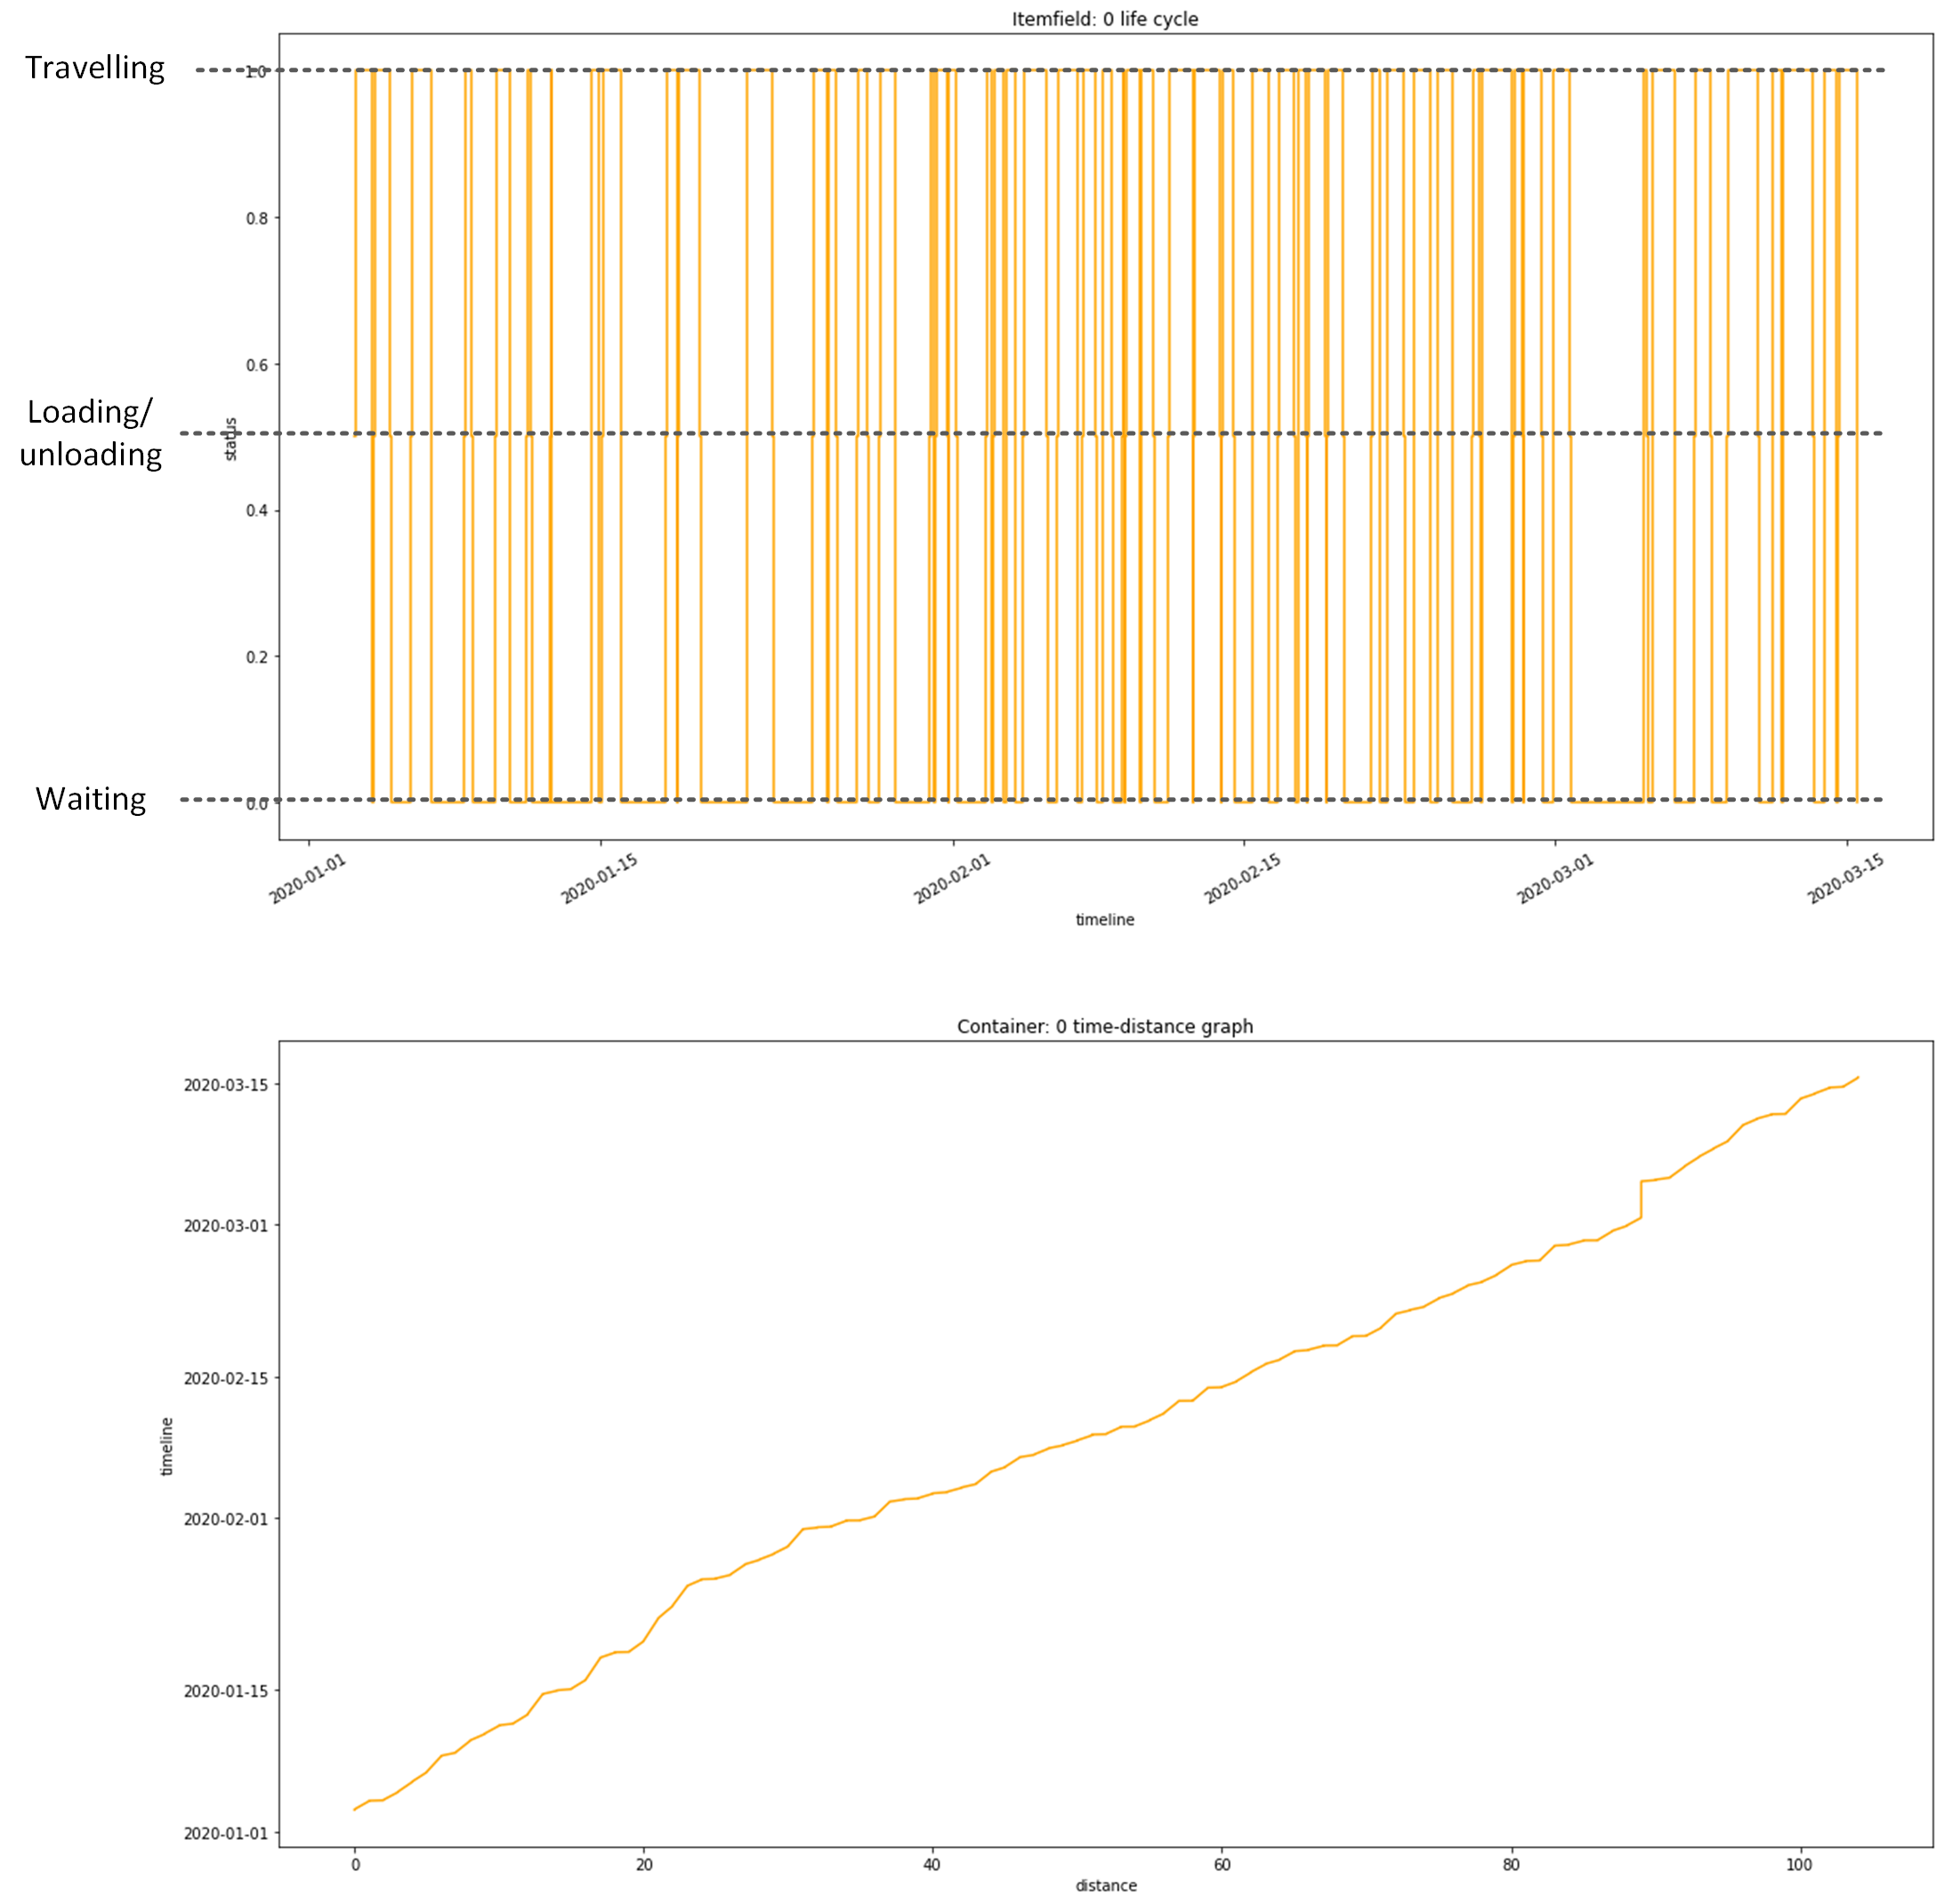
\includegraphics[width=0.9\textwidth]{SectionDistribution/control_figures/fig_lifecycle.png}
\captionsetup{type=figure}
\caption{Plot of the lifecycle, and the commercial speed of a HU according to the three states}
\label{fig_lifecycle}
\end{figure}

\paragraph{Vehicle Inventory analysis} \label{parVehicleInventoryAnalysis}

The analysis of the inventory position $WIP_v$ is important to identify the utilisation $U_v$ of a vehicle $v$, given its capacity $C_v$. It is necessary to know the planned/actual time windows at each terminal to infer the values of $WIP_v$, $U_v$, and $C_v$. Usually, the value of $C_v$ is fixed and depends on the type of vehicle or fleet. The other two values can be obtained by reconstructing the route of a vehicle $v$. Given a dataset with all the data, this is a heuristic procedure to get an estimate of the route.

\begin{itemize}
    \item Filter the dataset by a vehicle $v$;
	\item Select the actual or provisional time windows;
	\item Sort the values by the visiting time;
	\item Calculate the cumulative of the movements to estimate $WIP_j$.

\end{itemize}

When there are no known values of the $WIP_v(\tau)$ (e.g. from observation at time instant $\tau$), the best estimate is obtained by shifting to positive values the cumulative function of the movements. Otherwise, the cumulative function can be added forward, and backward to the known value of $WIP_j(\tau)$ (see Figure \ref{fig_vehicleInventory}); the inventory information is also represented as the weight of a graph $G(V,E)$. \footnote{The source code of Figure \ref{fig_vehicleInventory} is available \href{https://github.com/aletuf93/logproj/blob/master/examples/DIST_01\%20Supply\%20Chain\%20Assessment.ipynb}{here}.}

%insert figure fig_vehicleInventory
\begin{figure}[hbt!]
\centering
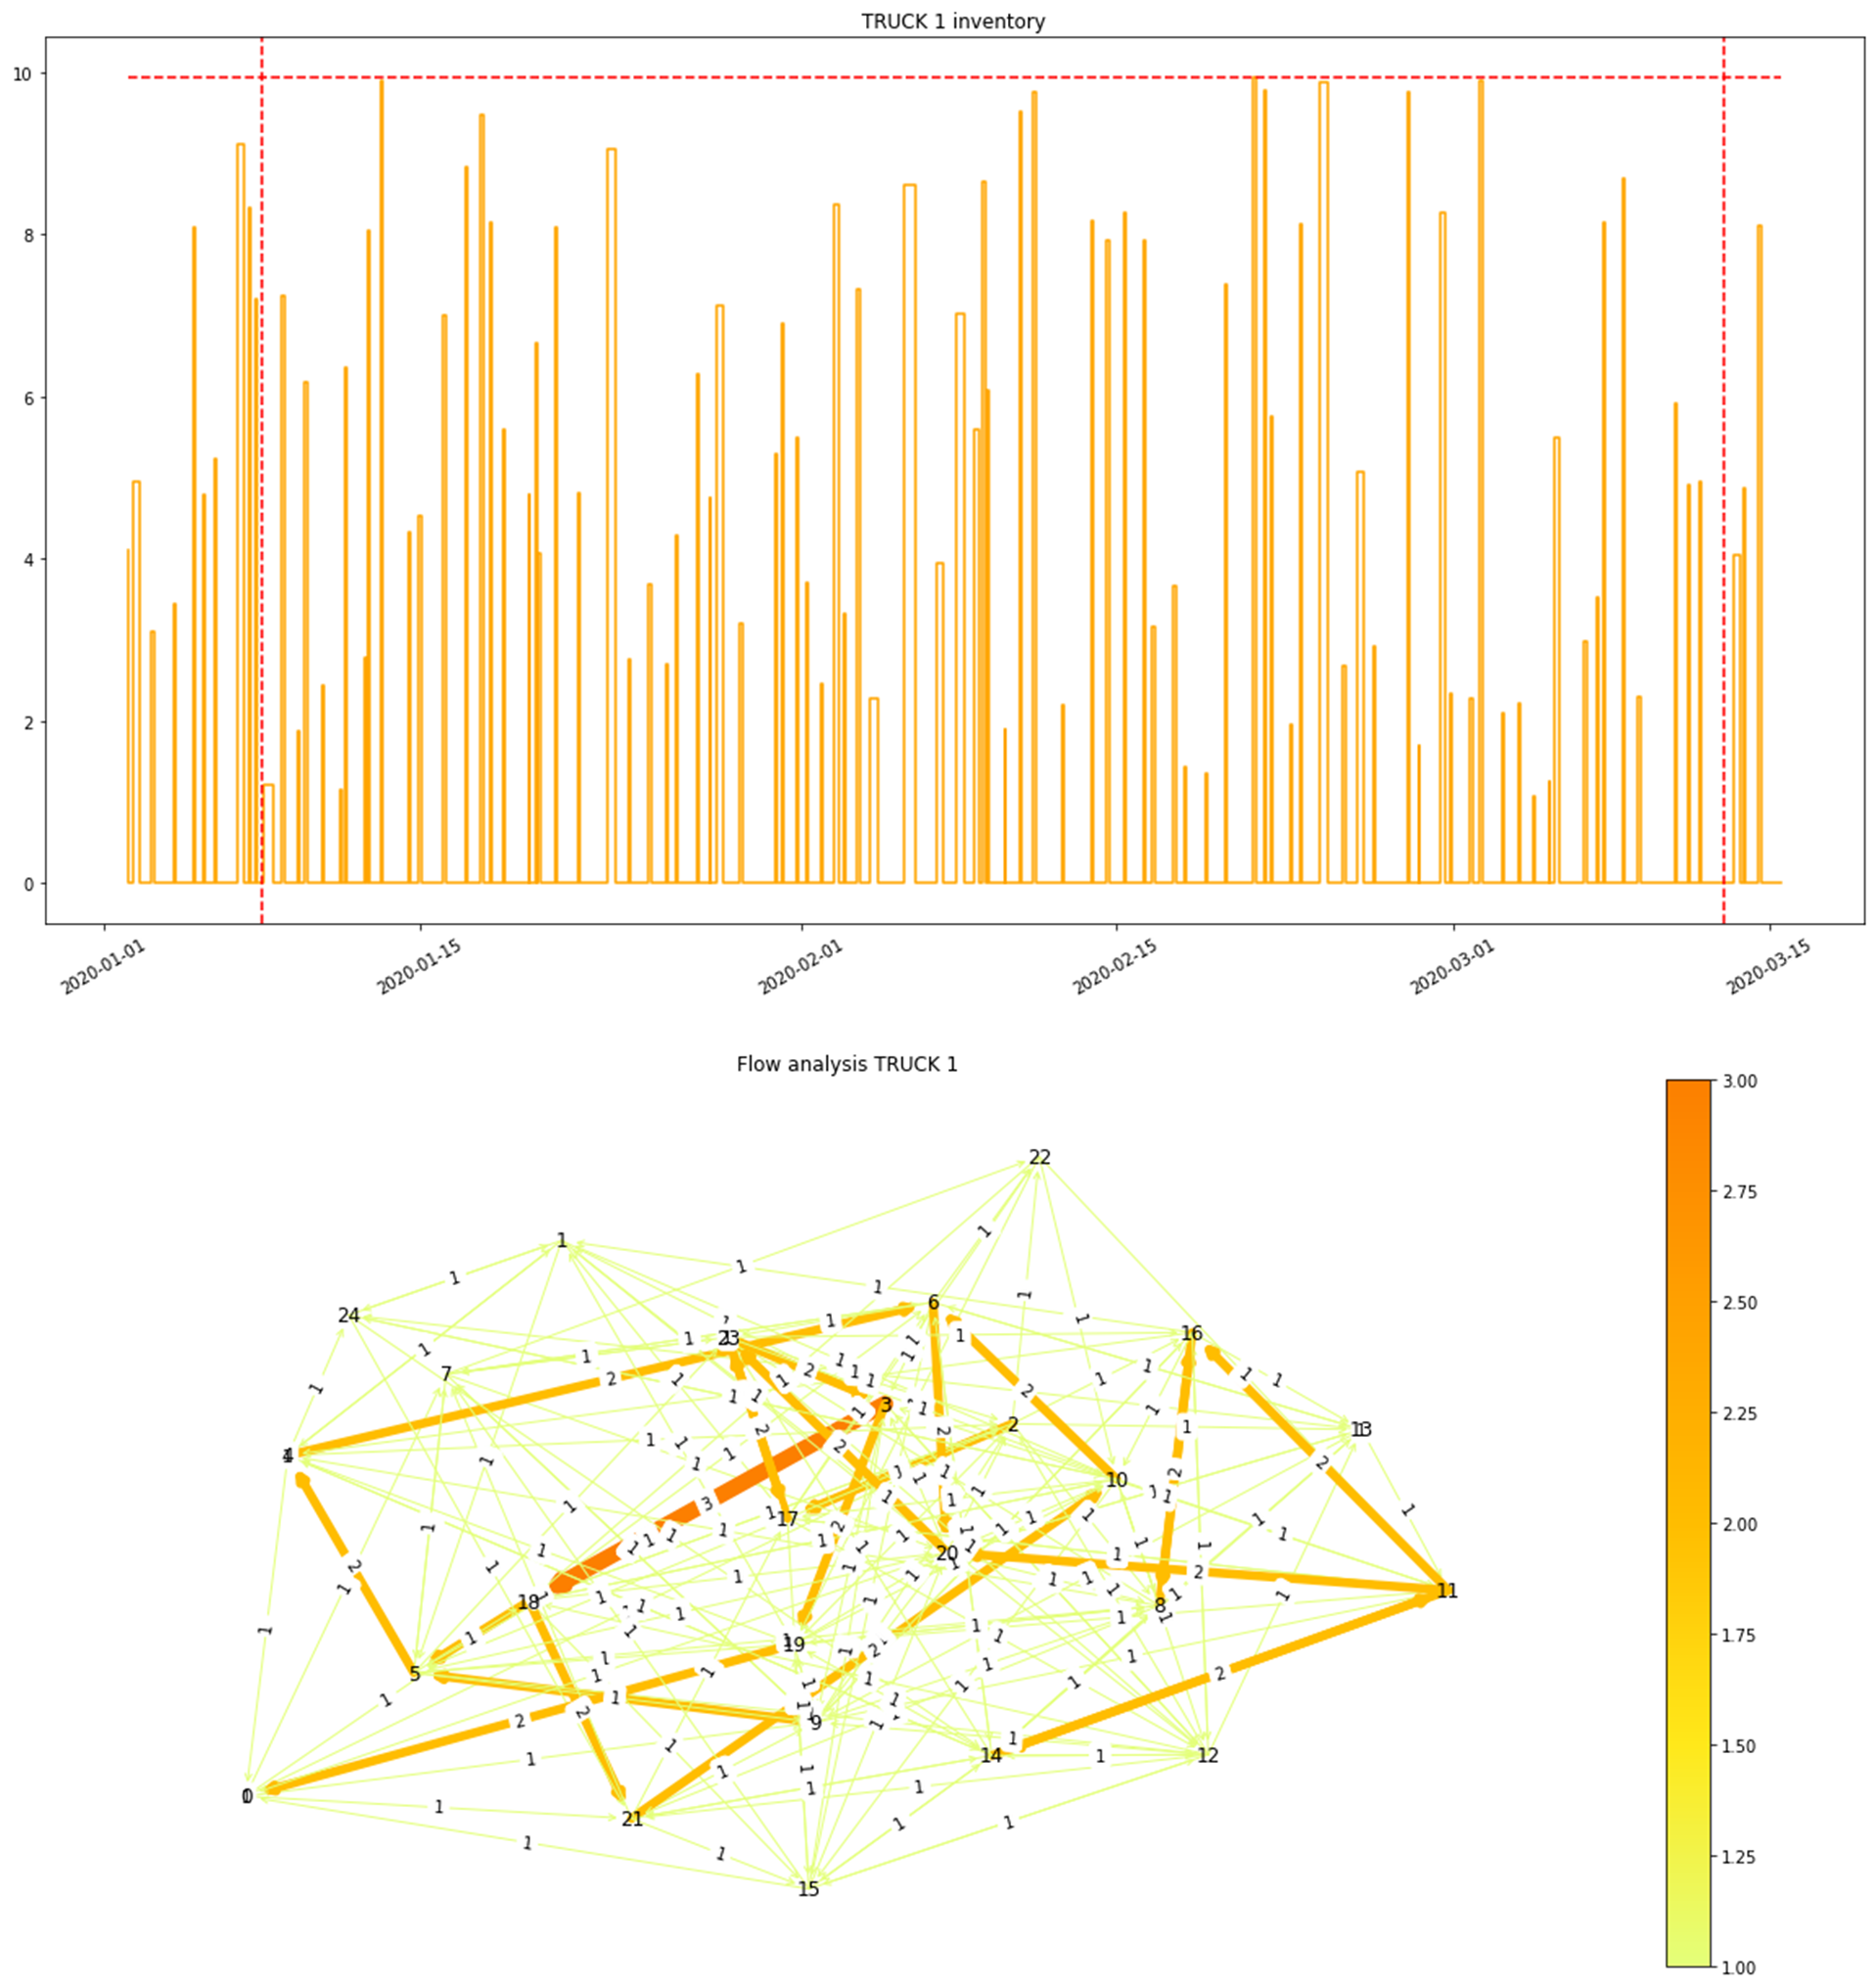
\includegraphics[width=0.9\textwidth]{SectionDistribution/control_figures/fig_vehicleInventory.png}
\captionsetup{type=figure}
\caption{The function of the inventory position of a vehicle in the time and space domains.}
\label{fig_vehicleInventory}
\end{figure}

\paragraph{Terminal Productivity analysis}
The network moves at speed defined by its terminals. It may sound weird that the speed of the distribution is imposed by fixed infrastructure, but it is easier the capacity of a terminal is the bottleneck of a distribution network, more than the capacity of a vehicle. It is always simpler to add a truck, a vessel, a train or even an air cargo than to add loading and discharging capacity of these vehicles.\par

By collecting, for each movement, the information on the provisional and actual time windows, it is possible to say a lot on the planned and actual behaviour of the terminals. Figure \ref{fig_terminalLinearProductivity} illustrates a scatterplot of the planned time windows of a terminal. \footnote{The source code of Figure \ref{fig_terminalLinearProductivity} is available \href{https://github.com/aletuf93/logproj/blob/master/examples/DIST_01\%20Supply\%20Chain\%20Assessment.ipynb}{here}.} The x-axis identifies the span of the time windows, while the y-axis the amount of HUs loaded or discharged. The plot identifies two patterns, almost linearly distributed. This pattern uncovers that the terminal may use one or two cranes at the same time to load/discharge a vehicle.

%insert figure fig_terminalLinearProductivity
\begin{figure}[hbt!]
\centering
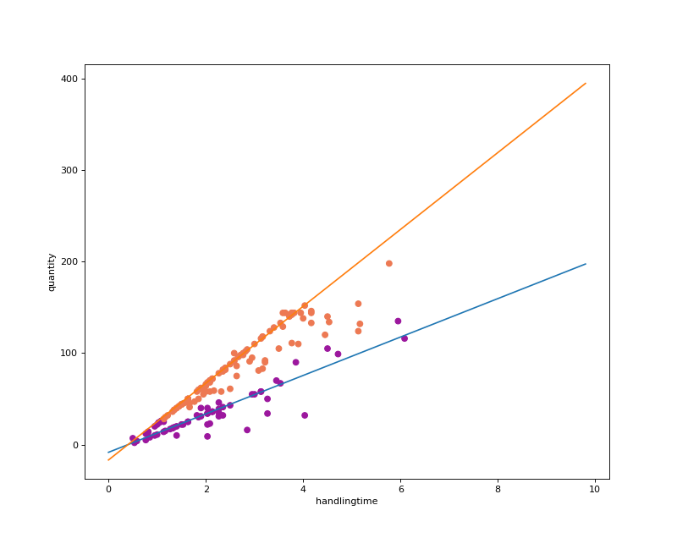
\includegraphics[width=0.6\textwidth]{SectionDistribution/control_figures/fig_terminalLinearProductivity.png}
\captionsetup{type=figure}
\caption{Productivity plot of a terminal.}
\label{fig_terminalLinearProductivity}
\end{figure}

This data reveals information on the capacity $C_j$ of a terminal $j$. The inventory position $WIP_j$ can be estimated with the same procedure illustrated in \ref{parVehicleInventoryAnalysis} by filtering on terminals, and not on vehicles. The throughput of a terminal usually depends on the time of the day. This information can be revealed by grouping the movements of a terminal on a specific day hour (see Figure \ref{fig_terminalProductivity}). \footnote{The source code of Figure \ref{fig_terminalProductivity} is available \href{https://github.com/aletuf93/logproj/blob/master/examples/DIST_01\%20Supply\%20Chain\%20Assessment.ipynb}{here}.}

%insert figure fig_terminalProductivity
\begin{figure}[hbt!]
\centering
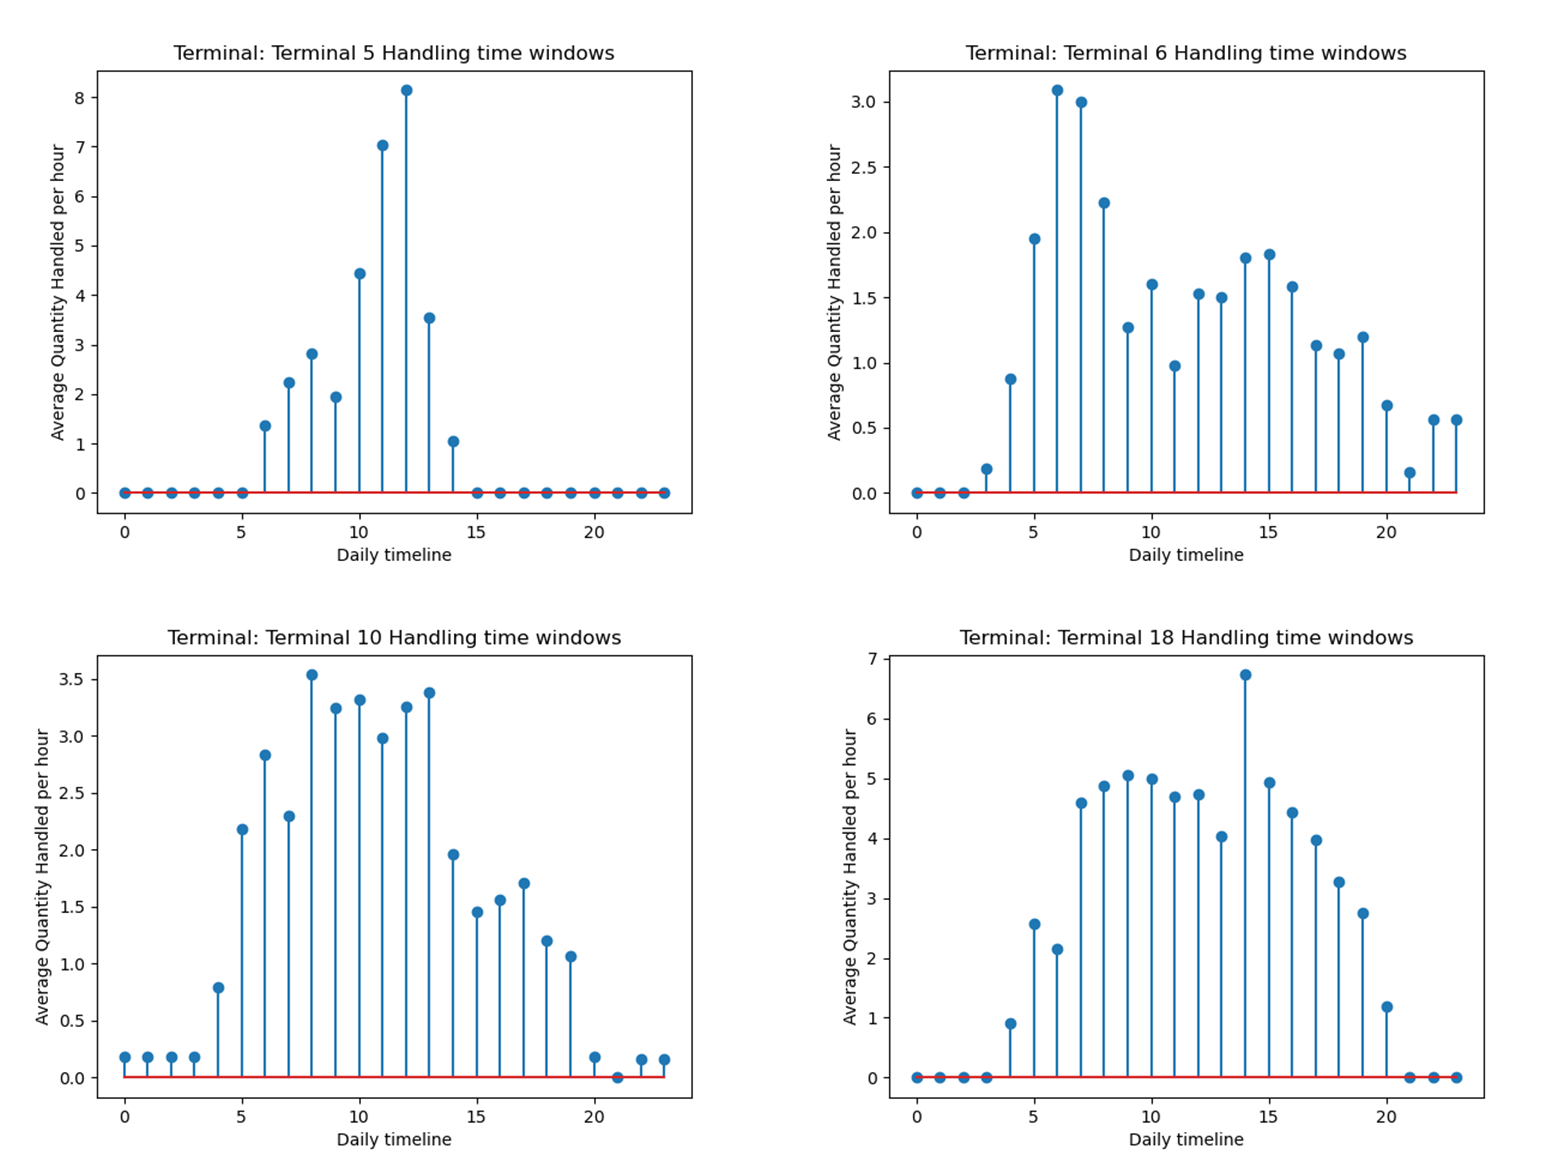
\includegraphics[width=0.9\textwidth]{SectionDistribution/control_figures/fig_terminalProductivity.png}
\captionsetup{type=figure}
\caption{Productivity patterns of four terminals (planned, and actual).}
\label{fig_terminalProductivity}
\end{figure}

\clearpage
\subsubsection{Network profiling}

\paragraph{Workload geography cost function}

It is possible to represent a geographical cost function by matching together the pieces of information used in the previous paragraph and the geographical information (latitude and longitude) of the node of the network. In particular, the cost is represented by the quantity delivered at each node. Figure \ref{fig_graph_workload} illustrates the cost function using the map as a background to identify the geographical position and the size of the bubble to identify the intensity of the demand quantity. The colour of the bubble can represent the type of service (e.g., the type of the delivery node), or a gradient to represent the intensity.\footnote{The source code of Figure \ref{fig_graph_workload} is available \href{https://github.com/aletuf93/logproj/blob/master/examples/DIST_02\%20Location\%20assessment.ipynb}{here}.}

%insert figure fig_graph_workload
\begin{figure}[hbt!]
\centering
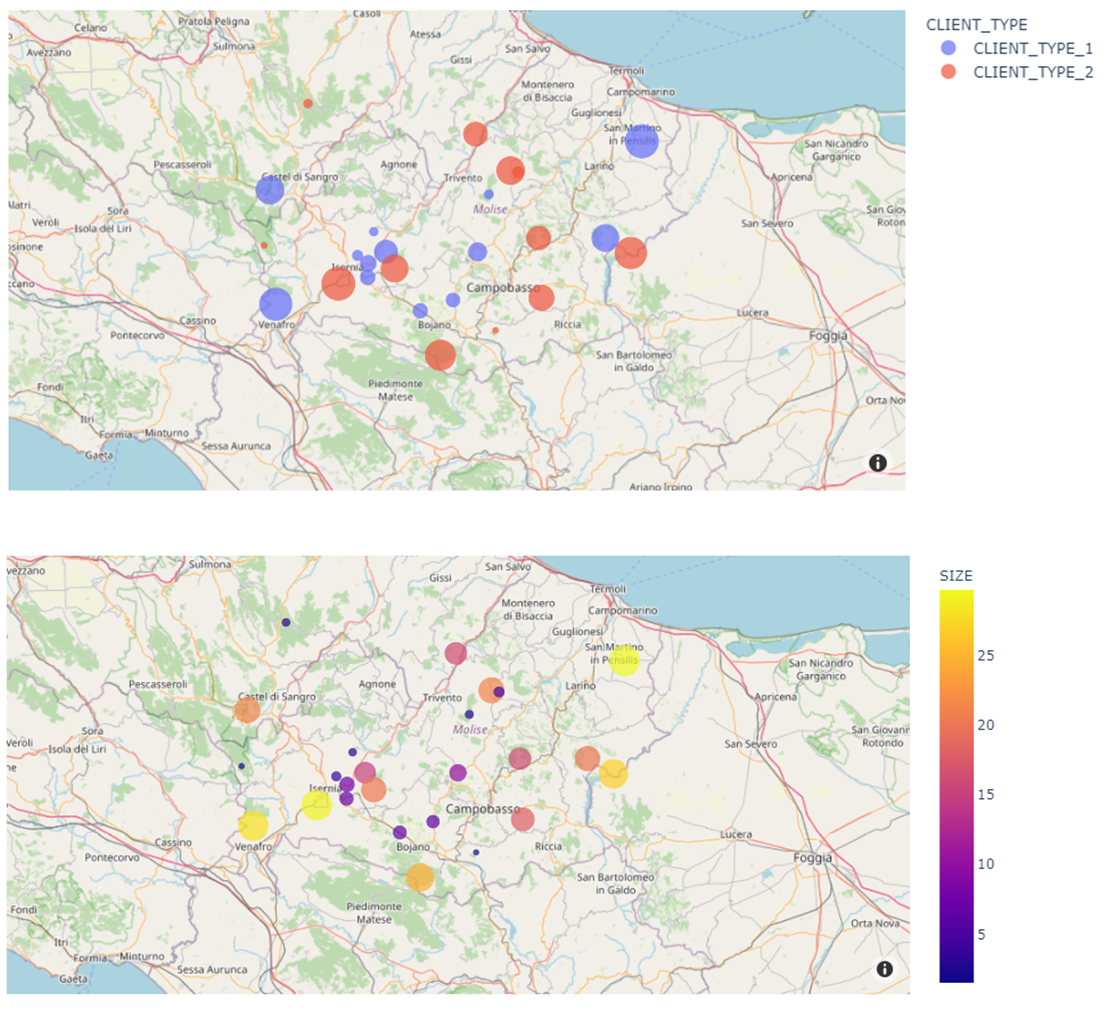
\includegraphics[width=0.9\textwidth]{SectionDistribution/control_figures/fig_graph_workload.png}
\captionsetup{type=figure}
\caption{Workload of the network represented on a map.}
\label{fig_graph_workload}
\end{figure}

\paragraph{Network centre of mass}

It is possible to define the centre of mass of the network, by considering the quantities, and the coordinates of the demand nodes of the network. Figure \ref{fig_graph_center_of_mass} compares the position of the centre of mass and the location of the plants serving the network.\footnote{The source code of Figure \ref{fig_graph_center_of_mass} is available \href{https://github.com/aletuf93/logproj/blob/master/examples/DIST_02\%20Location\%20assessment.ipynb}{here}.}

%insert figure fig_graph_center_of_mass
\begin{figure}[hbt!]
\centering
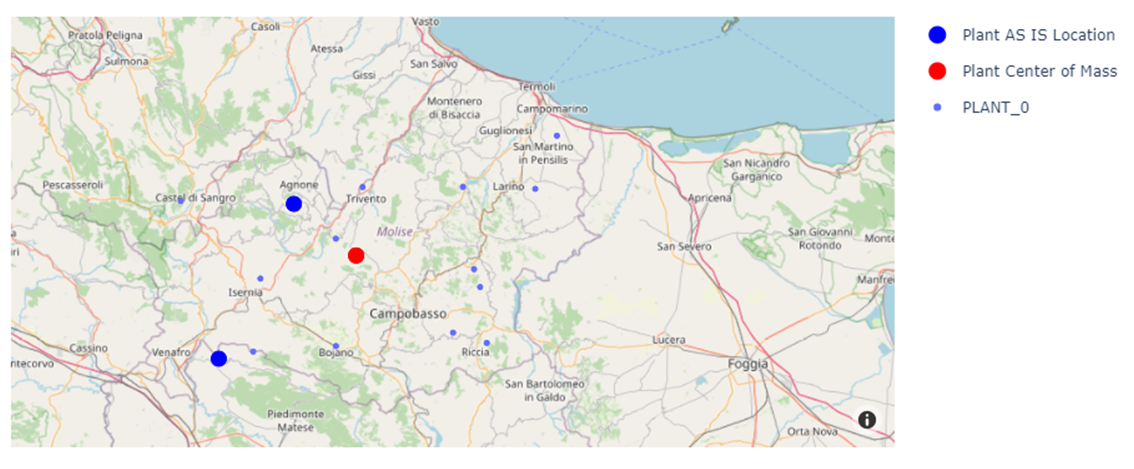
\includegraphics[width=1.0\textwidth]{SectionDistribution/control_figures/fig_graph_center_of_mass.png}
\captionsetup{type=figure}
\caption{Current location of the plants of the network, and centre of mass.}
\label{fig_graph_center_of_mass}
\end{figure}

\paragraph{Demand geographical covering}
It is possible to identify with different colours the node served by a specific plant of the network to identify how the production covers the demand on a geographical profile. Figure \ref{fig_graph_covering} illustrates the covering of the network.\footnote{The source code of Figure \ref{fig_graph_covering} is available \href{https://github.com/aletuf93/logproj/blob/master/examples/DIST_02\%20Location\%20assessment.ipynb}{here}.}

%insert figure fig_graph_covering
\begin{figure}[hbt!]
\centering
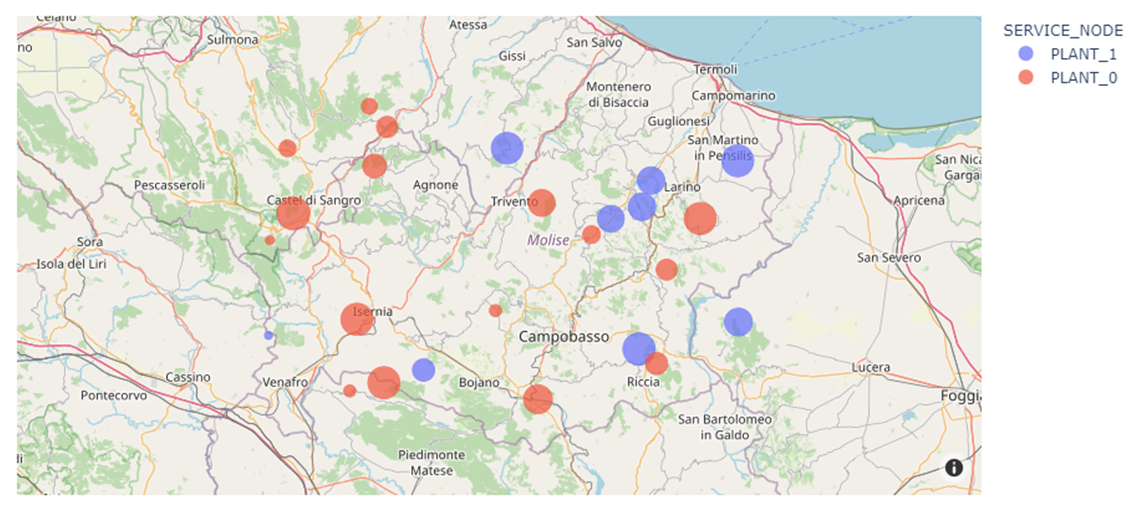
\includegraphics[width=0.9\textwidth]{SectionDistribution/control_figures/fig_graph_covering.png}
\captionsetup{type=figure}
\caption{Covering of the network. Different colours identify nodes served by different facilities.}
\label{fig_graph_covering}
\end{figure}

\paragraph{Road graph analyses}
Finally, it is possible to consider the road graph $G(V,E)$ of the network to perform analysis on the real distances. The top of Figure \ref{fig_road_graph} illustrates the edges of the graph. The subplot on the left uses rays to connect the nodes of the network exchanging the more significant amount of HUs. The subplot on the right use a colour gradient to identify the arcs travelled the most by the vehicles of the network.\footnote{The source code of Figure \ref{fig_road_graph} is available \href{https://github.com/aletuf93/logproj/blob/master/examples/DIST_02\%20Location\%20assessment.ipynb}{here}.}

%insert figure fig_road_graph
\begin{figure}[hbt!]
\centering
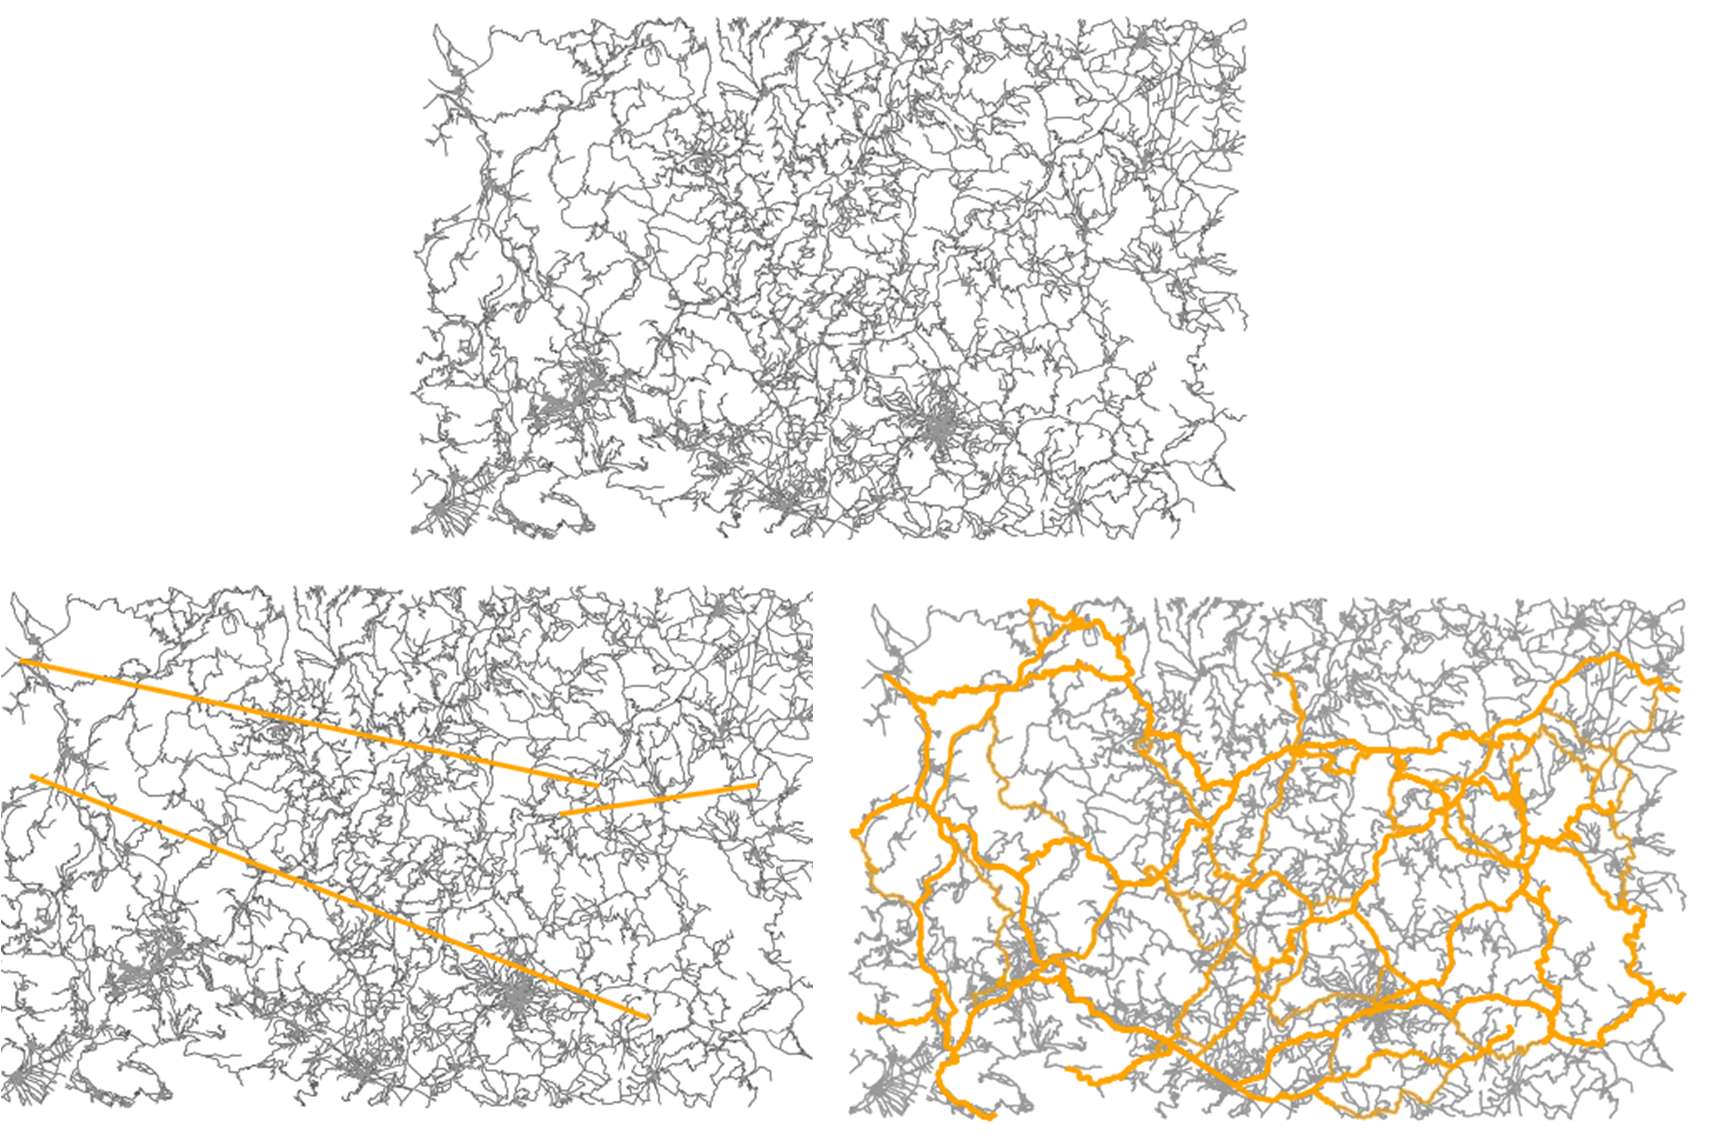
\includegraphics[width=0.9\textwidth]{SectionDistribution/control_figures/fig_road_graph.png}
\captionsetup{type=figure}
\caption{Road graph analyses.}
\label{fig_road_graph}
\end{figure}





\section{Workload prediction (P9)} \label{secDistWorkloadPrediction}
In a distribution network, it is crucial to forecast demand. The demand can be expressed in terms of:
\begin{itemize}
    \item the number of orders (i.e. the workload).
    \item the inventory of a vehicle (i.e. the available space to allocate to handling units).

\end{itemize}

We introduce model-driven methods to forecast the number of orders, and data-driven methods to deal with the prediction of the available space of a vehicle.

\subsection{Model-driven methods (PD2)}
Model-driven methods to forecast the workload are provided by the statistical analysis of the time series. When dealing with order data of a distribution network, it is possible to obtain a time series by:
\begin{enumerate}
    \item considering the timestamp of the dataset;
	\item cleaning the data by removing outliers;
	\item grouping and summing the quantities of the dataset by the timestamps;
	\item resampling the dataset to obtain an equispaced series $y$ (e.g. weekly, daily or hourly).

\end{enumerate}

At this stage, the series $y$ is consistent and can be used to feed prediction models as the time series decomposition (see section \ref{secTimeSeriesDecomposition}), ARIMA models (see section \ref{secARIMA}), Fourier analysis to detect seasonality (see section \ref{secFourier}), or other prediction models (e.g. fbprophet). Any of these models always provides:
\begin{itemize}
    \item the predicted value in a future time lag;
    \item a confidence interval.

\end{itemize}

It is always necessary to consider the confidence interval. When it is too wide, the model does not provide robust predictions. In this case, it is possible to tune the model with different hyperparameters, provide additional data, or change the model.\footnote{The logproj package provides methods to deal with workload predictions \href{https://github.com/aletuf93/logproj/blob/master/examples/LOG_02\%20Demand\%20prediction.ipynb}{here}.}


\subsection{Data-driven methods (PD1)}

As well as in storage and production system, forecasts on the number of movements (i.e. the number of HUs to handle) is essential for all the actors of a supply chain ~\cite{Moon2019}. Another crucial variable is the inventory position of a vehicle $v$, important to assign transportation orders to vehicle. These forecasts are made by using time series methods; nevertheless, the $WIP(t)$, is more incline to be affected by multiple factors, than the movements function. For this reason, machine learning algorithms are suitable to approach the predictions of the $WIP(t)$.\par

Once the route of a vehicle $v$, and its $WIP_v$ have been estimated, as illustrated in \ref{secDistOperationsProfiling}, it is possible to train learning models for the prediction of the inventory position of the vehicle. In particular, the residual capacity $r_j\left(t\right)=C_j-WIP_j(t)$ is of interest to investigate if a vehicle could handle more HUs than the ones already assigned to it. Learning models can be trained by using a training dataset $X^e$ containing information on the route $e$ (each row of the dataset is an arc travelled by a vehicle):
\begin{itemize}
    \item the id of the vehicle;
    \item the capacity of the vehicle;
    \item the node of departure;
    \item the time of departure;
    \item the node of arrival;
    \item the time of arrival.

\end{itemize}

While the target variable is represented by $WIP_j(t)$. The input dataset $X^e$ contains many date and time information. Learning models work approximating functions, i.e. they need only numerical values as inputs. For this reason, pre-processing is necessary to convert timestamps and categorical variables. Timestamps are transformed using $sin$ and $cos$ functions to separate year, month, days, hours and minutes in different attribute, preserving a measure of proximity between them (e.g. 00.01 is hugely close to 23.59 even if the digits representing the timestamp are at the opposite of the hours and minute domains). This transformation produces nine numerical features for each timestamp (one representing the years, two representing the month numbers, two representing the day numbers, two representing the hours, two representing the minutes). Categorical variables are converted to dummy column having value one if the observation has the value of the column, zero otherwise. This conversion produces a number of additional columns to the dataset $X^e$ equal to the number of categories of a categorical variable.\par

At this stage, man learning algorithms can be trained to approximate the value of $WIP_j(t)$. Any of the algorithms in chapters \ref{chapLinearRegression}, and \ref{cahpNonLinear} can be used, e.g. linear regression, lasso, ridge regression, elastic net, regression tree, random forest, gradient boosting, AdaBoost, support vector regression and single perceptron neural network. It is recommended to implement a validation procedure, as the cross-validation (see \ref{supervisedLearning}) and to choose a proper loss function (e.g. the MSE).\par

If the value of the MSE is low enough to support robust predictions, the model can be used to support decisions and to allocate capacity in advance. There is an additional parameter to consider to evaluate the performance of a model. When the model is trained, it produces an error with a fixed amount of data. When the model is deployed, this amount of data may vary. For this reason, it is crucial to consider the learning curve of a model. Learning curves track the value of the loss function (e.g. the MSE) depending on the amount of input data. Each algorithm runs several times with a different size of the input dataset randomly bootstrapped from the complete dataset $X^e$. An example of learning curves is presented in Figure \ref{fig_learningCurves}. The x-axes represent the number of records used to feed the learning algorithm (i.e. from 10\% to 100\% of the input dataset) while the y-axes indicate the average MSE produced by the algorithms with 5-folds CV.

%insert figure fig_learningCurves
\begin{figure}[hbt!]
\centering
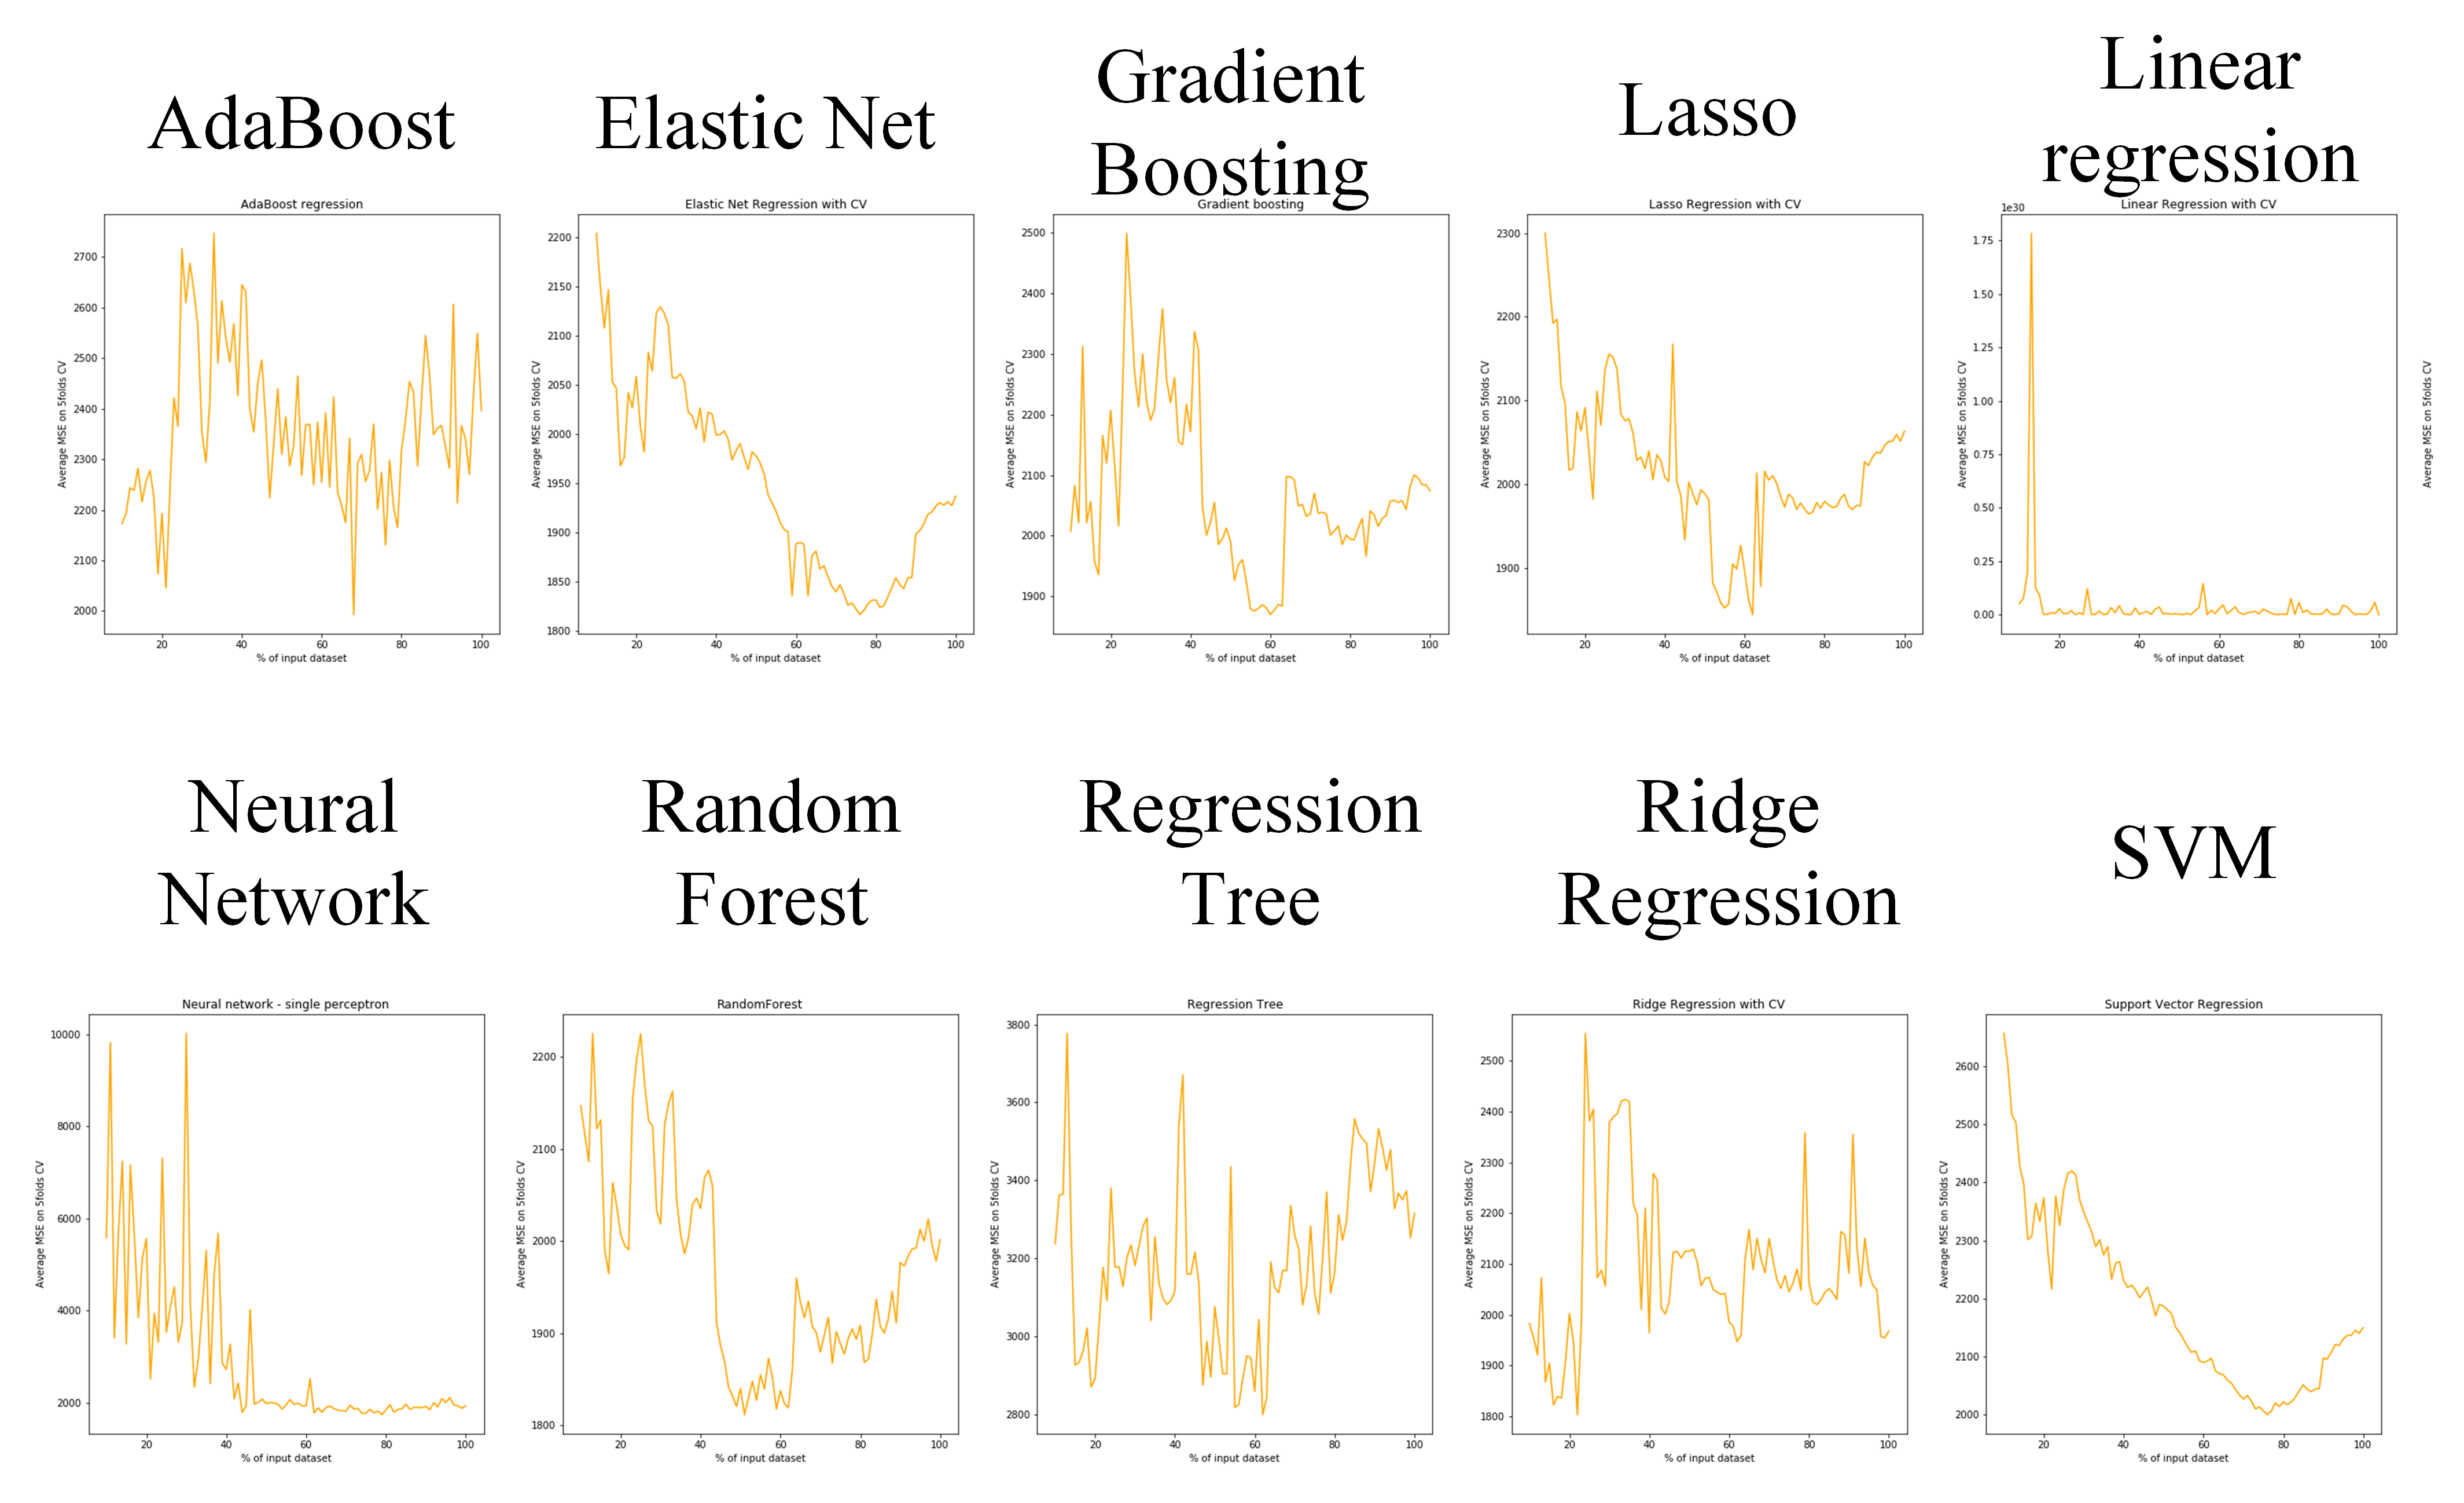
\includegraphics[width=0.9\textwidth]{SectionDistribution/control_figures/fig_learningCurves.png}
\captionsetup{type=figure}
\caption{Example of the learning curves of regression algorithms to predict the residual capacity of a vehicle.}
\label{fig_learningCurves}
\end{figure}

The example shows that many algorithms (i.e., neural network, gradient boosting, random forest and elastic net) tend to significantly reduce the MSE while increasing the size of the dataset. For this reason, the model built by these algorithms may have significant potential in practice fed using bigger datasets than the one used in this example.\footnote{The logproj package provides methods to deal with inventory predictions \href{https://github.com/aletuf93/logproj/blob/master/examples/LOG_02\%20Demand\%20prediction.ipynb}{here}.}


\section{Vehicle choice \& synchromodality (P2)}

The choice of an adequate vehicle to transport HUs from an origin to a destination can heavily affect the performance of the supply chain network in terms of the level of service and environmental impact. This problem is called \textit{synchromodality} when the choice is performed online, i.e. without a predefines association between the HU and the vehicle (e.g. truck, train, barge). Recent literature put a strong effort into developing synchromodality models. For the sake of brevity, we introduce an example inspired to the operations of a logistic platform, i.e. a company with a business model based on platform economy aiming at simplifying the operations of a distribution network (see section \ref{secLogPlatform}). \par

\subsection{Data-driven methods (PS2)}
We simulate the operations of a logistic platform by measuring the performance of the network using the transportation cost. The platform has to assign a set of containers to transportation services using barges or truck, where transportation of a container by truck costs 1.3 times more than a barge ~\cite{Fu2010,Konings2003}. For simplicity, we consider a single barge sailing the distribution network. The platform prefers to assign containers to the barge since it is cheaper than the truck. For this reason, their objective is the maximisation of the number of containers successfully transported by barge.

The platform uses a prediction model $\Pi$ to forecast the inventory position of the barge, defining the available capacity $\mu^{pred}$ of the barge in terms of available container slots. The accuracy of the available capacity is measured using the standard deviation $\sigma^{pred}$. The more accurate the prediction model $\Pi$, the lower $\sigma^{pred}$. The platform assigns a container to a truck when there is no space on a barge, based on $\mu^{pred}$; or when the real available capacity $\mu^{real}<\mu^{true}$. The assignments performed by the platform can be wrong due to bad predictions of the model $\Pi$. In particular, a type I error is made when a container is allocated to barge when the barge is already full (i.e. false positive prediction); a type II error is made when a container is allocated to a truck when the barge has space (i.e. false negative prediction). Figure \ref{fig_confusionMatrixPlatform} identifies all the possible outcomes of the prediction model $\Pi$. 


\begin{figure}[hbt!]
\centering
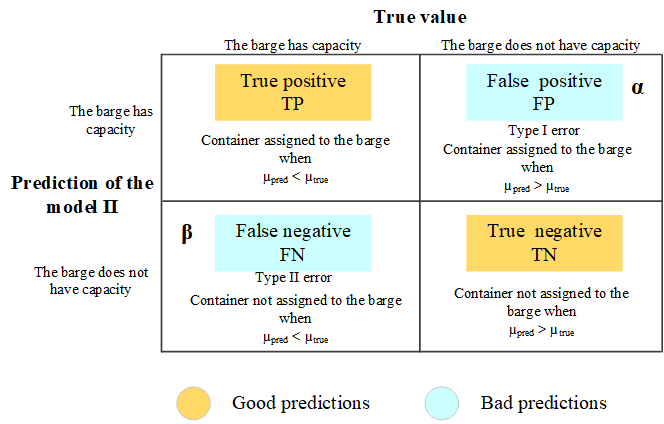
\includegraphics[width=0.9\textwidth]{SectionDistribution/control_figures/fig_confusionMatrixPlatform.png}
\captionsetup{type=figure}
\caption{Confusion matrix of a predictive model for synchromodality.}
\label{fig_confusionMatrixPlatform}
\end{figure}


We implemented a simulation to investigate the impact of the accuracy $\sigma^{pred}$ of the model $\Pi$ on the performance of the platform, by measuring:


\begin{itemize}
    \item the number of containers $\alpha$ assigned to the barge when $\mu^{pred}>\mu^{true}$ (i.e. the number of false positives);
    \item the number of containers $\beta$ assigned to trucks due to wrong predictions, when $\mu^{pred}<\mu^{true}$ (i.e. the number of false negatives);
    \item the total cost of the transportation service;
    \item the level of service, measured as the probability that the platform successfully assign a container to a barge (i.e. the percentage of true positives).
    
\end{itemize}


The simulation varies the accuracy of the predictions $\sigma^{pred}$ in a range from 0 to $\mu^{real}$. Figure \ref{fig_synchromodality} illustrates the outcome of the simulation, having on the x-axes the variation coefficient $\frac{\sigma^{pred}}{\mu^{true}}$, and the KPIs identified above on the y-axes, for each plot. The graph reveals that when the model $\Pi$ has higher accuracy in the prediction of the inventory position of the barge (i.e. the state $\Lambda$), the platform performs better, with a lower number of false positives and false negatives. This has a positive outcome on the level of service of the platform, and on the total transportation cost of the network.



\begin{figure}[hbt!]
\centering
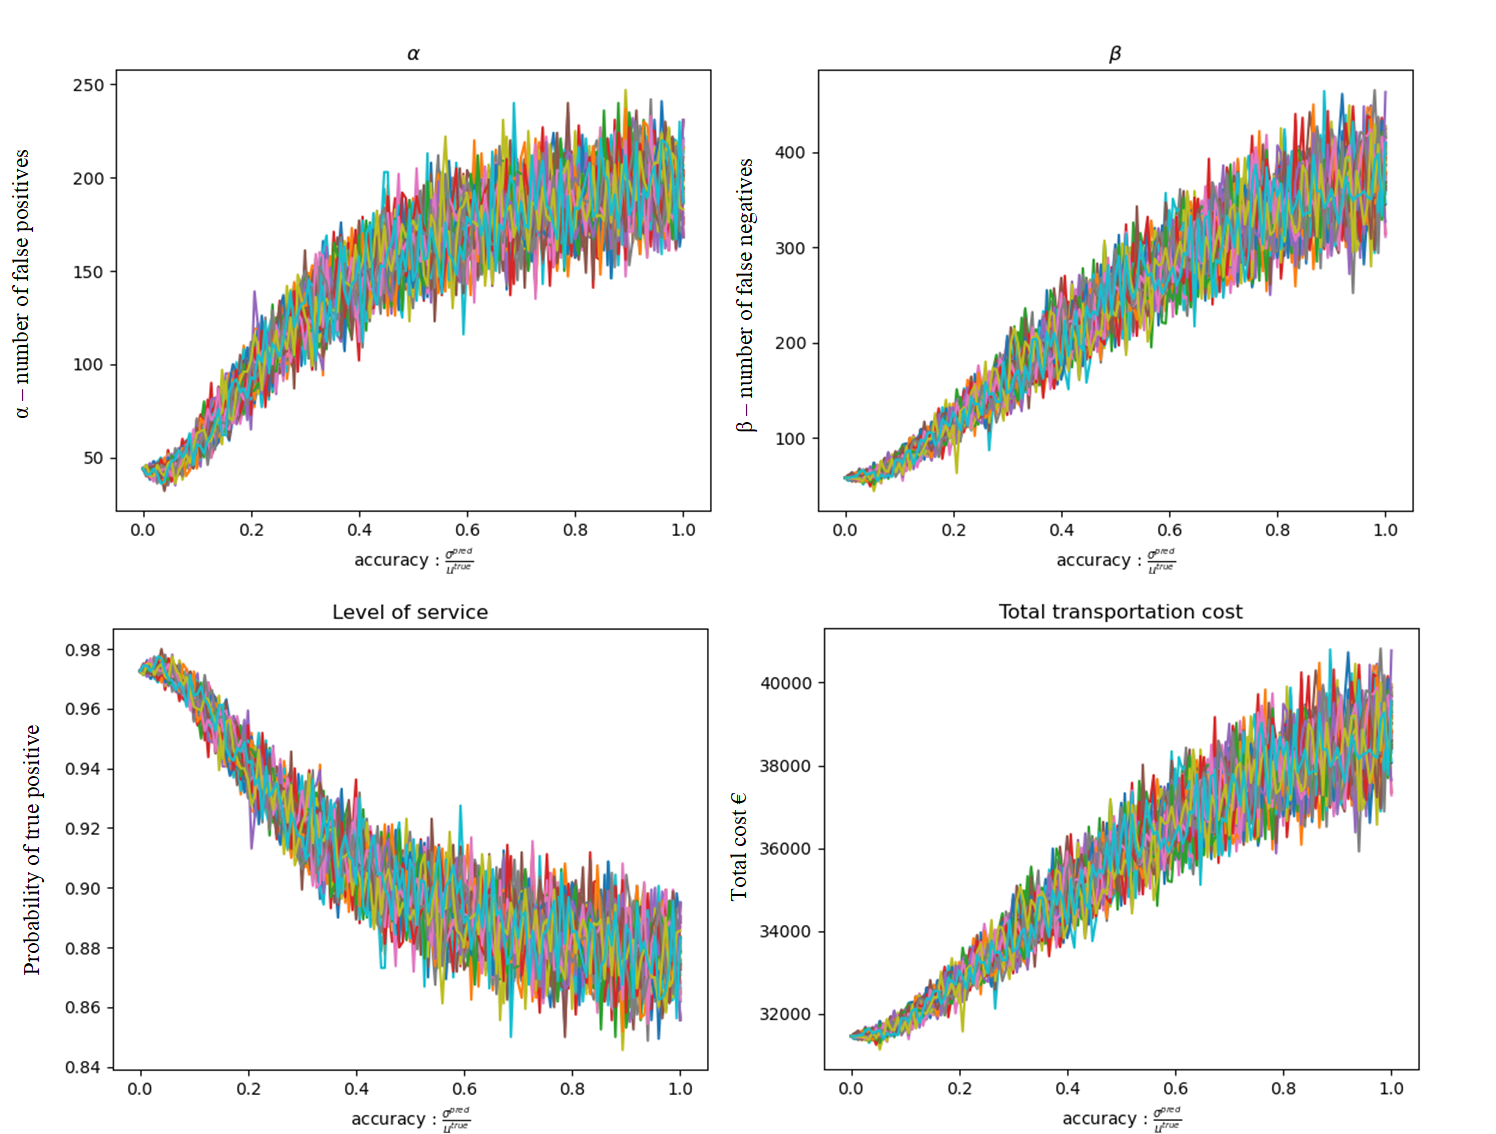
\includegraphics[width=0.9\textwidth]{SectionDistribution/control_figures/fig_synchromodality.png}
\captionsetup{type=figure}
\caption{Results of the simulation of the operations of a logistic platform}
\label{fig_synchromodality}
\end{figure}



This example shows that good prediction models targeting the inventory position of a barge can improve the level of service of the platform itself, and reduce the total transportation cost of a barge network. Differently from single actors of the supply chain, logistic platforms have the data and the possibility to implement these methodologies. The service they can deliver with this information is not only for their clients (e.g. the barge operators). Other stakeholders like terminals, shipper, and port authorities, can benefit from the information produced by the platforms. \par

\section{Vehicle routing (P10)}

Vehicle routing is a prescriptive problem to assign HUs to vehicles and define vehicle routes such that the distribution cost is minimised. We consider, first the problem from a classic and model-driven operation research perspective.

\subsection{Model-driven methods (PS1)} \label{secVRPmodelDriven}

This paragraph considers three different operations research approaches. The first is the travelling salesman problem (TSP), aiming at the definition of the cheapest route connecting all the nodes of a graph (regardless of the resource capacity). Then, the vehicle routing problem (VRP) is introduced using a traditional descriptive model and a smarter solving strategy using column generation.

\subsubsection{Separation algorithm for the TSP}

We do not introduce the descriptive model of the TSP since it can be found in almost any operation research book. We start illustrating a smarter procedure to solve it by separation (see \ref{secDuality}). Let consider the parameter $d_a$ be the cost of travelling the arc $a=(i,j)$. Let introduce the variables:

\begin{equation}
   \begin{split}
   w_a=\left\{
                \begin{array}{ll}
                  1\ & if\ arc\ \left(i,j\right)\ is\ included\ in\ the\ solution \\
                  0 & otherwise\\
                \end{array}
              \right.
   \end{split}
\end{equation}

\begin{equation}
   \begin{split}
   w_i=\left\{
                \begin{array}{ll}
                  1\ & if\ vertex\ i\ is\ included\ in\ the\ solution \\
                  0 & otherwise\\
                \end{array}
              \right.
   \end{split}
\end{equation}

The TSP problem is defined as follows.

\begin{equation}
\min{\sum_{a\in A}{w_ad_a}}
\label{dist_TSP_objectiveFunction}
\end{equation}

\begin{equation}
\sum_{a\in\delta^+(i)}{w_a=w_i, \forall\ i\in V}
\label{dist_TSP_constr_2}
\end{equation}

\begin{equation}
\sum_{a\in\delta^-(i)}{w_a=w_i, \forall\ i\in V}
\label{dist_TSP_constr_3}
\end{equation}

\begin{equation}
\sum_{i\in V}{w_i=N}
\label{dist_TSP_constr_4}
\end{equation}

\begin{equation}
w_a,\ w_i\in{0,1}
\label{dist_TSP_constr_5}
\end{equation}

The objective function (\ref{dist_TSP_objectiveFunction}) aims at the minimisation of the distribution cost. Constraints (\ref{dist_TSP_constr_2}), and (\ref{dist_TSP_constr_3}) impose to chose arcs both to enter and exit a vertex $i$, constraints (\ref{dist_TSP_constr_4}) impose to visit all the vertices, constraint (\ref{dist_TSP_constr_5}) impose integrality of the decision variables. A model set using equations (\ref{dist_TSP_objectiveFunction})-(\ref{dist_TSP_constr_5}) may produce a solution with multiple sub-tours. A set of sub-tour elimination constraints is needed to avoid this behaviour. The number of sub-tours in a graph can be exponential. For this reason, there is an exponential number of constraints to add to the problem (\ref{dist_TSP_objectiveFunction})-(\ref{dist_TSP_constr_5}). Models with an exponential number of constraints may take forever to reach optimality. For this reason, we relax this constraint and use a separation procedure adding one-by-one violated sub-tour elimination constraints to the model.\par

We introduce an optimisation problem called \textit{separation problem} to find a sub-tour elimination constraint $S^\ast$ violated by the initial problem. The problem has variables:

\begin{equation}
   \begin{split}
   y_i=\left\{
                \begin{array}{ll}
                  1\ & if\ vertex\ i\in S^\ast\\
                  0 & otherwise\\
                \end{array}
              \right.
   \end{split}
\end{equation}

\begin{equation}
   \begin{split}
   z_a=\left\{
                \begin{array}{ll}
                  1\ & if\ arc\ \left(i,j\right)\in S^\ast\\
                  0 & otherwise\\
                \end{array}
              \right.
   \end{split}
\end{equation}

The solution $z_a^\ast$ of the following separation problem is used to identify a sub-tour elimination constraint which is violated by the solution of the initial problem $w_a^\ast$. The separation problem is defined as follows:

\begin{equation}
\min{\sum_{i\in V}{y_i-\ \sum_{a\in A}{w_a^\ast z_a}}}
\end{equation}

\begin{equation}
\sum_{i\in V\ } y_i\le2
\end{equation}

\begin{equation}
\sum_{i\in V\ } y_i\geq N-2
\end{equation}

\begin{equation}
y_i\le z_a, \forall a=\left(i,j\right)\in A
\end{equation}

\begin{equation}
y_j\le z_a, \forall a=\left(i,j\right)\in A
\end{equation}

\begin{equation}
z_a\le y_i+y_j-1, \forall a=\left(i,j\right)\in A
\end{equation}

\begin{equation}
z_a,y_i\in{0,1}
\end{equation}

When the separation problem produces a solution value less than, or equal to '1', a constraint 
\begin{equation}
\sum_{a\in A(S^\ast)}{z_a^\ast>\sum_{i\in{V(S}^\ast)}{y_i-1}}
\end{equation}
is added to the initial problem. Then the initial problem is solved again (with the relaxation of the sub-tour elimination constraints), and the solution goes again to the separation problem. This algorithm stops when the separation problem does not produce additional constraints to add to the original problem. At this point, the initial problem is solved to optimality using a minimal number of sub-tour elimination constraints produced by the separation problem.

\subsubsection{Descriptive model for the VRP}
The most comprehensive prescriptive model in the field of distribution networks is an evolution of the TSP taking care of the capacity of the vehicle visiting the vertices ~\cite{Accorsi2017d}. This is the vehicle routing problem (VRP). One of the most complex and comprehensive versions of this problem is the VRP with pickup and deliveries and time windows (VRPPDTW). The VRPPDTW is modelled considering:
\begin{itemize}
    \item a fleet of vehicles $v\in B$;
	\item a set of pickup and delivery orders $o\in O$ to serve;
	\item a set of pickup nodes $j\in P$ and a set of delivery nodes $j\in D$ defining a directed graph $G\left(V,A\right)$ where $V=P\bigcup D$ and $\left(i,j\right)\in A$.
\end{itemize}

In this paragraph, we introduce a VRPPDTW problem to maximise the profit of a shipper of cargo vessels ~\cite{Accorsi2018}. Despite the scope of the problem, its formulation is valid for any distribution network with pickup and deliveries and time windows. The parameters of the problem are illustrated in Table \ref{tab_VRP_vessels}.

\begin{figure}[hbt!]
\centering
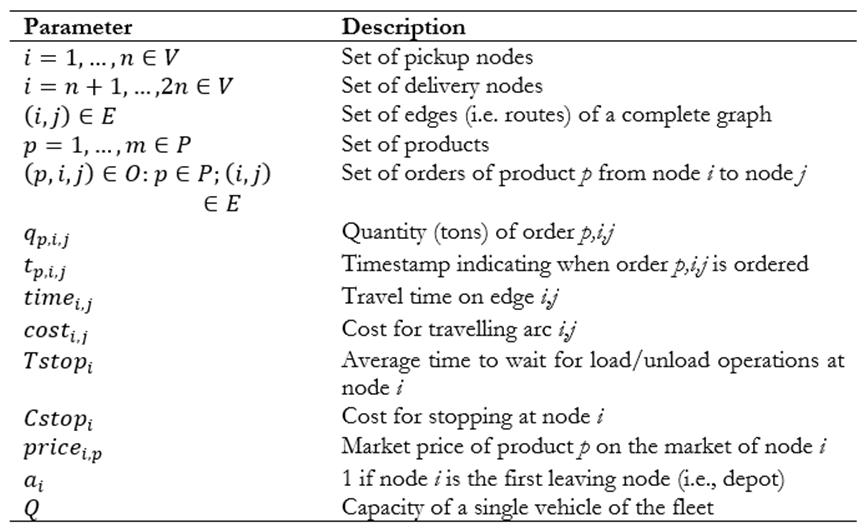
\includegraphics[width=0.9\textwidth]{SectionDistribution/control_figures/tab_VRP_vessels.png}
\captionsetup{type=table}
\caption{Parameters of the VRP problem.}
\label{tab_VRP_vessels}
\end{figure}



\clearpage
The mathematical model admits the following decision variables.

\begin{equation}
   \begin{split}
   x_{i,j}=\left\{
                \begin{array}{ll}
                  1\ & if\ arc\ i,j\ is\ travelled\\
                  0 & otherwise\\
                \end{array}
              \right.
   \end{split}
\end{equation}

\begin{equation}
   \begin{split}
   v_i=\left\{
                \begin{array}{ll}
                  1\ & if\ node\ i\ is\ visited\\
                  0 & otherwise\\
                \end{array}
              \right.
   \end{split}
\end{equation}

\begin{equation}
   s_i=timestamp\ \ upon\ leaving\ node\ i
\end{equation}

\begin{equation}
   \begin{split}
   u_{p,i,j}=\left\{
                \begin{array}{ll}
                  1\ & if\ order\ p,i,j\ is\ served\\
                  0 & otherwise\\
                \end{array}
              \right.
   \end{split}
\end{equation}

\begin{equation}
   {load}_{p,i}=upper\ bound\ of\ the\ total\ pickup\ quantity\ upon\ leaving\ node\ i
\end{equation}

\begin{equation}
   {unload}_{p,i}=upper\ bound\ of\ the\ total\ delivered\ quantity\ upon\ leaving\ node\ i
\end{equation}

The feasible region is defined by the following sets of constraints.

\begin{equation}
\sum_{j}{x_{i,j}=v_i}, i\in V
\label{VRP_1}
\end{equation}

\begin{equation}
\sum_{i}{x_{i,j}=v_j}, j\in V
\label{VRP_2}
\end{equation}

\begin{equation}
s_i=0, i\in V:a_i=1
\label{VRP_3}
\end{equation}

\begin{equation}
s_j\geq s_i+time_{i,j}-M(1-x_{i,j}), \left(i,j\right)\in E;i,j\in V \backslash \{j:a_j=1\}
\label{VRP_4}
\end{equation}

\begin{equation}
s_j\le s_i+time_{i,j}+M(1-x_{i,j}), \left(i,j\right)\in E;i,j\in V \backslash \{j:a_j=1\}
\label{VRP_5}
\end{equation}

\begin{equation}
u_{p,i,j}\le v_i, (p,i,j\in O)
\label{VRP_6}
\end{equation}

\begin{equation}
u_{p,i,j}\le v_j, (p,i,j\in O)
\label{VRP_7}
\end{equation}

\begin{equation}
load_{p,i}=\sum_{j}{q_{p,i,j}{\times u}_{p,i,j}}, p\in P,\ i\in V:a_i=1\ 
\label{VRP_8}
\end{equation}

\begin{equation}
\begin{split}
load_{p,j}\geq-M\left(1-x_{i,j}\right)+load_{p,i}+\sum_{k} q_{p,j,k}{\times u}_{p,j,k}, \\
p\in P\ \left(i,j\right)\in E;i,j\in V \backslash \{j:a_j=1\}\\
\end{split}
\label{VRP_9}
\end{equation}

\begin{equation}
unload_{p,i}=0, p\in P,\ i\in V:a_i=1
\label{VRP_10}
\end{equation}

\begin{equation}
\begin{split}
unload_{p,j}\geq-M\left(1-x_{i,j}\right)+unload_{p,i}+\sum_{k} q_{p,k,j}{\times u}_{p,k,j},\\
p\in P\ \left(i,j\right)\in E;i,j\in V\ \backslash \{j:a_j=1\}\\
\end{split}
\label{VRP_11}
\end{equation}

\begin{equation}
0\le\sum_{p}{load_{p,i}-unload_{p,i}\le Q}, i\in V
\label{VRP_12}
\end{equation}

\begin{equation}
u_{p,i,j}\times t_{p,i,j}\le s_j+time_{i,j}, \left(p,i,j\right)\in O
\label{VRP_13}
\end{equation}

\begin{equation}
x_{i,j}\in{0,1}, \left(i,j\right)\in E
\label{VRP_14}
\end{equation}

\begin{equation}
v_i\in{0,1}, i\in V
\label{VRP_15}
\end{equation}

\begin{equation}
s_i\geq0, i\in V
\label{VRP_16}
\end{equation}

\begin{equation}
u_{p,i,j}\in{0,1}, (p,i,j)\in O
\label{VRP_17}
\end{equation}

\begin{equation}
{load}_{p,i,j}\geq0, (p,i,j)\in O
\label{VRP_18}
\end{equation}

\begin{equation}
{unload}_{p,i,j}\geq0, (p,i,j)\in O
\label{VRP_19}
\end{equation}

Constraints (\ref{VRP_1}) and (\ref{VRP_2}) ensure the route is continuous among nodes. Constraints (\ref{VRP_3}) set the leaving timestamp at the first node. Constraints (\ref{VRP_4}) and (\ref{VRP_5}) are used to track the leaving timestamp at each node. Constraints (\ref{VRP_6}) and (\ref{VRP_7}) impose a node must be visited to serve its orders. Constraints (\ref{VRP_8}) set the pickup value at the first node while constraints (\ref{VRP_9}) do the same for all the following. Constraints (\ref{VRP_10}) set the delivery value at the first node while constraints (\ref{VRP_11}) do the same for all the following. Constraints (\ref{VRP_12}) ensure the capacity is never exceeded, and constraints (\ref{VRP_13}) state that an order can be served when it comes before the picking node is visited. Constraints (\ref{VRP_14}), (\ref{VRP_15}), (\ref{VRP_16}), (\ref{VRP_17}), (\ref{VRP_18}), (\ref{VRP_19}) set the values of the variables.\par

The maximisation of the profit of the shipper is chosen as objective function.

\begin{equation}
\sum_{p,i,j}{q_{p,i,j}\times u_{p,i,j}\times p r i c e_{p,i,j}-\sum_{i}{Cstop_i\times v_i}-\sum_{i,j}{c_{i,j}\times x_{i,j}\ }}
\end{equation}

This problem has been solved using the branch and bound algorithm to test its functionality on a toy instance (i.e. an extremely small instance of the problem). The toy instance network is composed of the nine vertices illustrated in the left of Figure \ref{fig_vesselsOptimal}. The right part of Figure \ref{fig_vesselsOptimal} illustrates the solution of the toy instance, similarly to the descriptive analytics illustrated in \ref{secDistOperationsProfiling}.

\begin{figure}[hbt!]
\centering
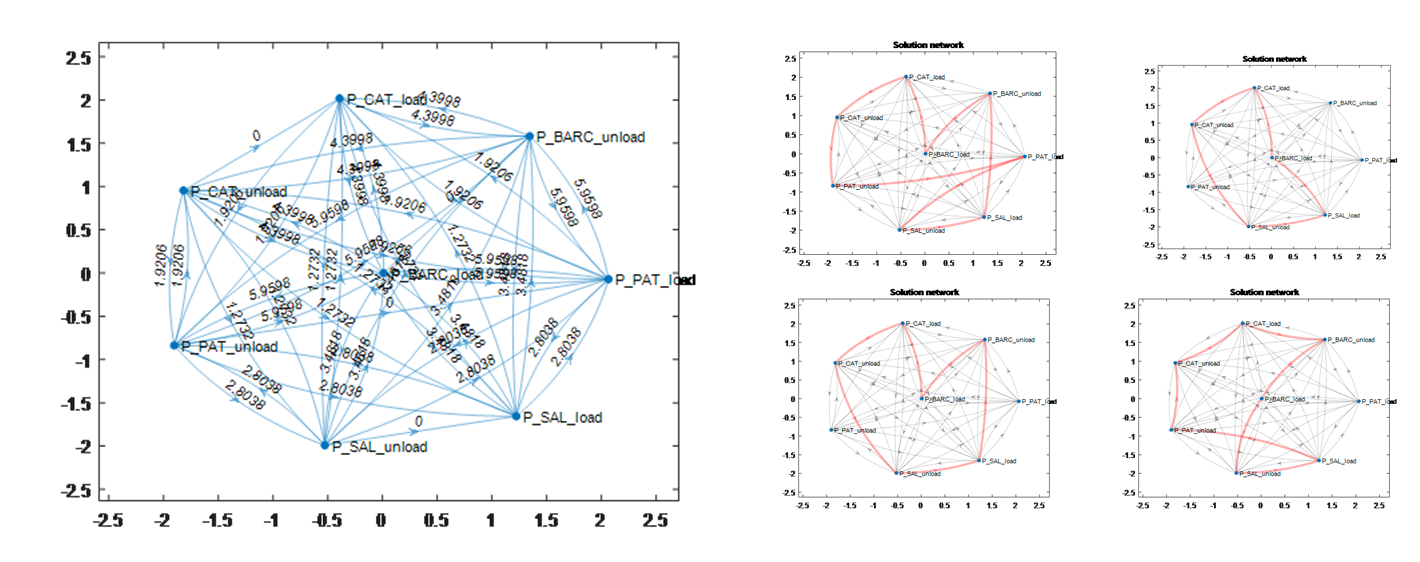
\includegraphics[width=0.9\textwidth]{SectionDistribution/control_figures/fig_vesselsOptimal.png}
\captionsetup{type=figure}
\caption{Solution of the toy instance of the VRP problem.}
\label{fig_vesselsOptimal}
\end{figure}

Since the problem involves time windows, for each route identified by the solution, it is possible to identify the timestamps of visit at the ports similarly to the analytics of \ref{secDistOperationsProfiling} (see Figure \ref{fig_vesselInventory}). 

\begin{figure}[hbt!]
\centering
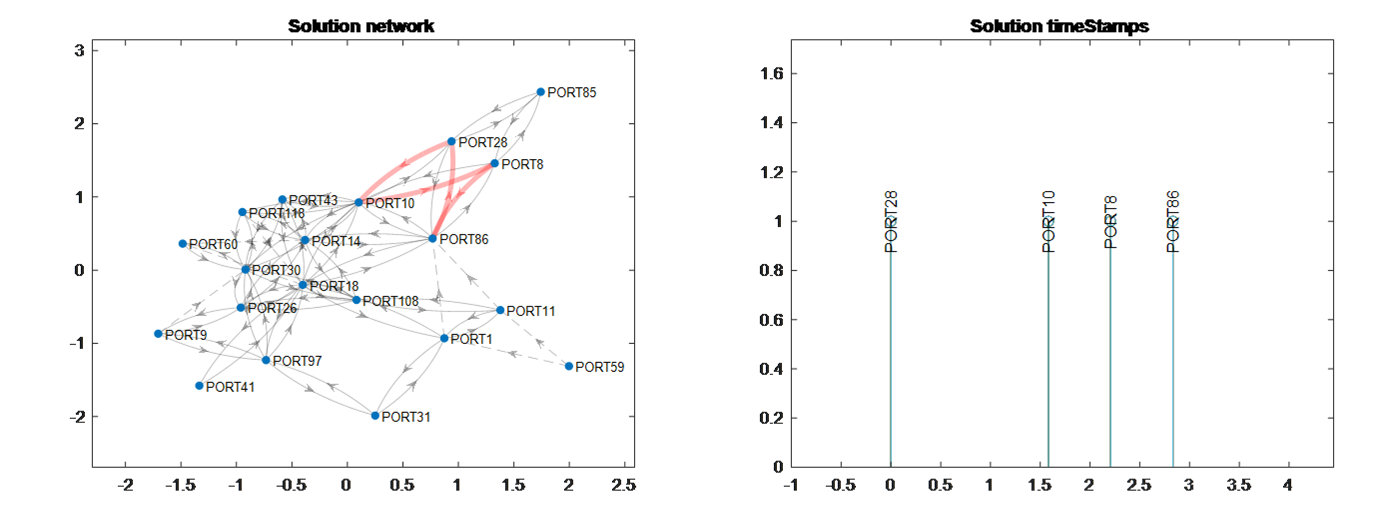
\includegraphics[width=0.9\textwidth]{SectionDistribution/control_figures/fig_vesselInventory.png}
\captionsetup{type=figure}
\caption{Descriptive analytics to evaluate the solution of the prescriptive problem.}
\label{fig_vesselInventory}
\end{figure}

It is crucial to utilise the same KPIs and analytics to evaluate both the actual scenario and the ones produced by prescriptive analytics.

\subsubsection{Column generation algorithms for the VRP}

Operations research proposes many descriptive models to address the vehicle routing problem (VRP). Unfortunately, even if easy to understand, they are hard to solve since VRP is NP-complete. Still being NP-complete, there are smart algorithm known as \textit{column generation algorithms} to expedite the research of the optimal solution. For this reason, we introduce this type of algorithms that works properly with relatively small networks (few hundreds of nodes).Let us consider the parameters of the problem presented in Table \ref{tab_VRP_colgen}.

\begin{figure}[hbt!]
\centering
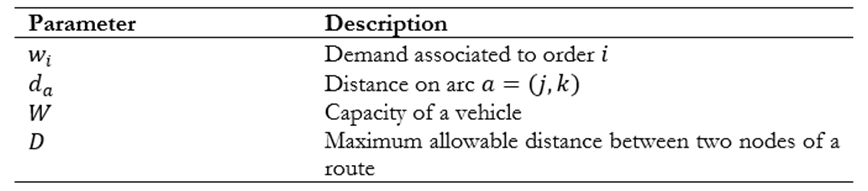
\includegraphics[width=0.9\textwidth]{SectionDistribution/control_figures/tab_VRP_colgen.png}
\captionsetup{type=table}
\caption{Parameters of the column generation algorithm for the VRP.}
\label{tab_VRP_colgen}
\end{figure}

We define a set $S$ containing all the feasible routes on the network (i.e. the routes respecting the capacity $W$, and where nodes are not farther than $D$.

\begin{equation}
    S=\left\{s\subseteq\left\{i=1,\ldots m\right\}:\sum_{i\in s}{w_i\le W},\ {MAX_{a:j,k\in s}{d}_a\le\ D}\ \right\}
\end{equation}

The optimal solution to the VRP is the solution to the set covering problem (SCP) called \textit{primal problem}, having the parameter $c_s$ to define the cost of the route $s$, and a variable:

\begin{equation}
   \begin{split}
   x_s=\left\{
                \begin{array}{ll}
                  1\ & if\ configuration\ s\ is\ selected\\
                  0 & otherwise\\
                \end{array}
              \right.
   \end{split}
\end{equation}

The primal problem is defined as follows.

\begin{equation}
   \min{c_sx}_S
\end{equation}

\begin{equation}
   \sum_{s\in S:i\in s}{x_s\geq1}, i=1,\ldots,m\ \ 
\end{equation}

\begin{equation}
    x_s\in\left\{0,1\right\}
\end{equation}

The SCP problem has an exponential number of variables that are unknown in advance (we do not know, at the beginning, all the feasible routes of set $S$). For this reason, we initialise the primal problem with a trivial feasible solution of the SCP (i.e. an identity matrix with a high cost $c_s$) and we use a dual problem to generate cheaper columns of the matrix. We relax the integrality of the primal problem and consider its \textit{dual problem}, as follows.

\begin{equation}
    \max{\pi_i}
\end{equation}

\begin{equation}
    \sum_{i\in S}{\pi_i\le c_s}, s\in S
    \label{VRP_colgen_toviolate}
\end{equation}

\begin{equation}
    \pi_i\geq0, i\in S
\end{equation}

At this point, we need to violate a constraint of the set (\ref{VRP_colgen_toviolate}). When this constraint exists, a cheaper column to add to the $S$ exists as well for the theorem of optimality by separation (see section \ref{secDuality}). We use an optimisation model to find the violated constraint.

\begin{equation}
   \begin{split}
   \mu_i=\left\{
                \begin{array}{ll}
                  1\ & if\ i\ belongs\ to\ column\\
                  0 & otherwise\\
                \end{array}
              \right.
   \end{split}
\end{equation}

\begin{equation}
    \max{\sum_{i=1}^{m}{\mu_i(\pi_i-c_i)}}
\end{equation}

\begin{equation}
    \sum_{i=1}^{m}{\pi_iw_i\le W}
\end{equation}

\begin{equation}
    \mu_i\geq\ z_a , a=(i,j)
\end{equation}

\begin{equation}
    \mu_j\le z_a , a=(i,j)
\end{equation}

\begin{equation}
    \mu_i+\mu_j-1\le z_a , a=(i,j)
\end{equation}

\begin{equation}
    z_ad_a\le D , a=(i,j)
\end{equation}

\begin{equation}
    \pi_i,z_a\in{0,1} , a=\left(i,j\right);i,j=1,\ldots,m
\end{equation}

If this model produces a solution value $\sum_{i=1}^{m}{\mu_i(\pi_i-c_i)}>0$, a column with profit is found, and it is added to the set $S$ of the SCP. Otherwise, the set $S$ contains all the routes to find the optimal solution to the problem. The solution of the primal SCP problem reveals the solution to the VRP. \par

Similarly, it is possible to use this approach to solve the VRPPDTW maximising the profit of the shipper, illustrated in the previous paragraph using the descriptive model. Let consider the set packing problem with the following variables:

\begin{equation}
    C=set\ of\ all\ maximal\ orderset\ served\ by\ a\ feasible\ route
\end{equation}

\begin{equation}
   \begin{split}
   x_c=\left\{
                \begin{array}{ll}
                  1\ & if\ orderset\ c\ selected\\
                  0 & otherwise\\
                \end{array}
              \right.
   \end{split}
\end{equation}

The problem has a parameter $\gamma_c$, indicating the profit associated to the orderset (i.e.e the route) $c$. The primal problem is identified as:

\begin{equation}
    \max{\sum_{c\in C}{x_c\gamma_c}}
\end{equation}

\begin{equation}
    \sum_{c\in C:o\in c}{x_c\le1} , o\in O
\end{equation}

\begin{equation}
    x_c\in\left\{0,1\right\} , c\in C
\end{equation}

Let define the dual problem at:

\begin{equation}
    \max{\sum_{o\in O}\pi_o}
\end{equation}

\begin{equation}
    \sum_{o\in c}{\pi_o^ \le-\gamma_c} , c\in C
\end{equation}

\begin{equation}
    \pi_o^ \le0 , i\in O
\end{equation}

We are interested in finding a set $c$ such that:

\begin{equation}
    c:\sum_{o\in c}{\pi_o^\ast+\gamma_c>0}
\end{equation}

Let consider a column generation problem setting the value of the decision variable:

\begin{equation}
   \begin{split}
   y_o=\left\{
                \begin{array}{ll}
                  1\ & if\ order\ o\ in\ c \\
                  0 & otherwise\\
                \end{array}
              \right.
   \end{split}
\end{equation}

The problem is defined as follows:

\begin{equation}
    \max{\sum_{o\in O}{(\pi_o^\ast-profit_o)}y_o\ }-\sum_{i}{Cstop_i\times v_i}-\sum_{i,j}{c_{i,j}\times x_{i,j}\ }
\end{equation}

\begin{equation}
    profit_o\le q_{p,i,j}\times u_{p,i,j}\times price_{p,i,j} , o=\left(p,i,j\right)
\end{equation}

\begin{equation}
    u_{p,i,j}\le y_o\ , o=\left(p,i,j\right)
\end{equation}

Subject to all the constraints \ref{VRP_1} to \ref{VRP_19} defining the feasible region. Each time this problem is solved with a solution value greater than '0', a maximal orderset is found and added to the primal problem following the algorithm illustrated for the minimisation case.

\subsection{Data-driven methods (PS4)} \label{secDataDrivenRouting}

The models illustrated in the previous section are complex and extremely biased. Besides, they need long runtimes to produce an optimal solution. This running time and the hypotheses made to set the model (e.g. the linearity of all the behaviour described by the constraints) are hard to support in a real environment. \par

For this reason, we introduce a different approach, where the past observation of the network can help to find a solution to an online version of the VRP by using predictive algorithms. The models presented in \ref{secVRPmodelDriven} solve an offline version of the VRP, i.e. all the data are not only static but given before running the algorithm that solves the model. In practice, many parameters of the problem are unknown, or they change their value depending on many external factors. Finding an online solution of the VRP means finding a feasible assignment of a HU to a vehicle, given the current state of the system (i.e. the vehicles present in the network, their routes, and their available capacity). This can be seen as the Uber problem, who find a ride to share with other users, given a set of available cabs.\par

This is the perfect job for a logistic platform, collecting the data of different stakeholders of a distribution network. Let us consider, for example, a platform collecting the movements $M_o^{j,v}$ from different conveyance operators, where $o$ is a single transportation order, $j$ the origin terminal, and $v$ the vehicle. Let us define a state $\widetilde{\Lambda}(\tau)$ defined as the set of the inventory position of all the terminals $j$, and all the vehicles $v$ of the network at time instant $\tau$. If the logistic platform can estimate $\widetilde{\Lambda}(\tau)$, is it able to define if a vehicle has available capacity for an additional HU (i.e. a feasible solution of the online VRP). \par

The platform can estimate the inventory position of the barge, by using the movement function (using an algorithm similar to the one presented in section \ref{secInfoFramework}). Another source of information comes from the productivity function of the terminals $j$ (i.e. $P_j^{IN}$, and $P_j^{OUT}$). These two data sources can be matched together by using a Kalman filter, to improve the estimate $\widetilde{\Lambda}$. The number of movements $n_v$ observed for each single vehicle $v$ defines the completeness of $M_v(t)$, while the number of all the observations m defines the completeness of $P_j^{IN}$, and $P_j^{OUT}$ for each terminal $j$. Two estimators of $\widetilde{\Lambda}$ can, then, be obtained by using two different approaches:

\begin{itemize}
    \item ${\widetilde{\Lambda}}^M$, with an empirical approach, from the knowledge of the movements $M_j\left(t\right)$;
	\item ${\widetilde{\Lambda}}^K$, with a probabilistic approach, from the definition of kinematic models based on the speeds of the terminals given by $P_j^{IN}$, and $P_j^{OUT}$.

\end{itemize}

An empirical approach directly applies the equations (\ref{eqInvj}) and (\ref{eqInvv}). A probabilistic approach defines a kinematic model $K_j$ for each terminal $j$. $K_j({\delta^t,P}_j^{IN},P_j^{OUT},Prob_j^{OUT})$ returns the number of HUs loaded or offloaded when a barge stops at a terminal $j$ with a service time windows $\delta^t$. The model considers the probability distribution functions of the productivity $P_j^{IN}$ and $P_j^{OUT}$, and the probability that the terminal $j$ loads or offload containers $Prob_j^{OUT}$). \par

The Kalman filter (see section \ref{secKalmanFilter}) is introduced to mix the information from the empirical, and the probabilistic approach. A Kalman filter (KF) considers the input and outputs of a kinematic model, and it corrects the output value based on empirical measurements when they are available. The filter is suitable for a logistic platform since it can be continuously updated, allowing real-time implementations. The Kalman filter estimates the value of $\widetilde{\Lambda}(\tau)$ as a hidden state of a Markov model. Given the motion equation $K_j$ for each terminal $j$, the filter updates $\widetilde{\Lambda}\left(\tau\right)$ by considering the empirical measurements $M_o^{j,v}$. The use of the filter always improves the accuracy of $\widetilde{\Lambda}\left(\tau\right)$ obtained by using only the probabilistic approach. Nevertheless, it may be useless when $M_v(t)$ has an information content high enough to (e.g. when all the movements $M_o^{j,v}$ of a vehicle $v$ have been observed. 








%\clearpage
\bibliographystyle{ieeetr}
\bibliography{SectionDistribution/control_ref}